%Version 3.1 December 2024
% See section 11 of the User Manual for version history
%
%%%%%%%%%%%%%%%%%%%%%%%%%%%%%%%%%%%%%%%%%%%%%%%%%%%%%%%%%%%%%%%%%%%%%%
%%                                                                 %%
%% Please do not use \input{...} to include other tex files.       %%
%% Submit your LaTeX manuscript as one .tex document.              %%
%%                                                                 %%
%% All additional figures and files should be attached             %%
%% separately and not embedded in the \TeX\ document itself.       %%
%%                                                                 %%
%%%%%%%%%%%%%%%%%%%%%%%%%%%%%%%%%%%%%%%%%%%%%%%%%%%%%%%%%%%%%%%%%%%%%

%%\documentclass[referee,sn-basic]{sn-jnl}% referee option is meant for double line spacing

%%=======================================================%%
%% to print line numbers in the margin use lineno option %%
%%=======================================================%%

%%\documentclass[lineno,pdflatex,sn-basic]{sn-jnl}% Basic Springer Nature Reference Style/Chemistry Reference Style

%%=========================================================================================%%
%% the documentclass is set to pdflatex as default. You can delete it if not appropriate.  %%
%%=========================================================================================%%

%%\documentclass[sn-basic]{sn-jnl}% Basic Springer Nature Reference Style/Chemistry Reference Style

%%Note: the following reference styles support Namedate and Numbered referencing. By default the style follows the most common style. To switch between the options you can add or remove “Numbered” in the optional parenthesis. 
%%The option is available for: sn-basic.bst, sn-chicago.bst%  
 
%%\documentclass[pdflatex,sn-nature]{sn-jnl}% Style for submissions to Nature Portfolio journals
%%\documentclass[pdflatex,sn-basic]{sn-jnl}% Basic Springer Nature Reference Style/Chemistry Reference Style
%\documentclass[pdflatex,sn-mathphys-num]{sn-jnl}% Math and Physical Sciences Numbered Reference Style
%%\documentclass[pdflatex,sn-mathphys-ay]{sn-jnl}% Math and Physical Sciences Author Year Reference Style
%%\documentclass[pdflatex,sn-aps]{sn-jnl}% American Physical Society (APS) Reference Style
%%\documentclass[pdflatex,sn-vancouver-num]{sn-jnl}% Vancouver Numbered Reference Style
%%\documentclass[pdflatex,sn-vancouver-ay]{sn-jnl}% Vancouver Author Year Reference Style
%%\documentclass[pdflatex,sn-apa]{sn-jnl}% APA Reference Style
%%\documentclass[pdflatex,sn-chicago]{sn-jnl}% Chicago-based Humanities Reference Style

%%%% Standard Packages
%%<additional latex packages if required can be included here>
%\usepackage{newunicodechar}
%\newunicodechar{₀}{$_0$}
%\newunicodechar{₀}{$_0$}
%\usepackage[utf8]{inputenc}
%\newunicodechar{μ}{\textmu{}}

%\usepackage{graphicx}%
%\usepackage{multirow}%
%\usepackage{amsmath,amssymb,amsfonts}%
%\usepackage{amsthm}%
%\usepackage{mathrsfs}%
%\usepackage[title]{appendix}%
%\usepackage{xcolor}%
%\usepackage{textcomp}%
%\usepackage{manyfoot}%
%\usepackage{newunicodechar}
%\newunicodechar{₀}{$_0$}
%\newunicodechar{₁}{$_1$}
%\newunicodechar{₂}{$_2$}
%\newunicodechar{₃}{$_3$}
%\newunicodechar{₄}{$_4$}
%\newunicodechar{₅}{$_5$}
%\newunicodechar{₆}{$_6$}
%\newunicodechar{₇}{$_7$}
%\newunicodechar{₈}{$_8$}
%\newunicodechar{₉}{$_9$}
%\usepackage{newunicodechar}
%\newunicodechar{ᵗ}{\textsuperscript{t}}
%\newunicodechar{ʰ}{\textsuperscript{h}}
%\usepackage{newunicodechar}
%\newunicodechar{₀}{$_0$}
%\usepackage{textgreek}
%\usepackage{newunicodechar}
%\newunicodechar{−}{-}
%\usepackage{booktabs}%
%\usepackage{algorithm}%
%\usepackage{algorithmicx}%
%\usepackage{algpseudocode}%
%\usepackage{listings}%
%%%%

%%%%%=============================================================================%%%%
%%%%  Remarks: This template is provided to aid authors with the preparation
%%%%  of original research articles intended for submission to journals published 
%%%%  by Springer Nature. The guidance has been prepared in partnership with 
%%%%  production teams to conform to Springer Nature technical requirements. 
%%%%  Editorial and presentation requirements differ among journal portfolios and 
%%%%  research disciplines. You may find sections in this template are irrelevant 
%%%%  to your work and are empowered to omit any such section if allowed by the 
%%%%  journal you intend to submit to. The submission guidelines and policies 
%%%%  of the journal take precedence. A detailed User Manual is available in the 
%%%%  template package for technical guidance.
%%%%%=============================================================================%%%%

%% as per the requirement new theorem styles can be included as shown below
%\theoremstyle{thmstyleone}%
%\newtheorem{theorem}{Theorem}%  meant for continuous numbers
%%\newtheorem{theorem}{Theorem}[section]% meant for sectionwise numbers
%% optional argument [theorem] produces theorem numbering sequence instead of independent numbers for Proposition
%\newtheorem{proposition}[theorem]{Proposition}% 
%%\newtheorem{proposition}{Proposition}% to get separate numbers for theorem and proposition etc.

%\theoremstyle{thmstyletwo}%
%\newtheorem{example}{Example}%
%\newtheorem{remark}{Remark}%

%\theoremstyle{thmstylethree}%
%\newtheorem{definition}{Definition}%

%\raggedbottom
%%\unnumbered% uncomment this for unnumbered level heads

%\begin{document}

%\title[Article Title]{Article Title}

%%=============================================================%%
%% GivenName	-> \fnm{Joergen W.}
%% Particle	-> \spfx{van der} -> surname prefix
%% FamilyName	-> \sur{Ploeg}
%% Suffix	-> \sfx{IV}
%% \author*[1,2]{\fnm{Joergen W.} \spfx{van der} \sur{Ploeg} 
%%  \sfx{IV}}\email{iauthor@gmail.com}
%%=============================================================%%

\documentclass[9pt,twocolumn,twoside]{rilabRxiv}
% Use the documentclass option 'lineno' to view line numbers
\setlength{\marginparwidth}{2cm}
\usepackage[textsize=tiny,colorinlistoftodos]{todonotes}
\newcommand{\rra}[1]{\todo[inline,color=orange!30]{\textbf{rra:} #1}}
\definecolor{cornflowerblue}{rgb}{0.39, 0.58, 0.93}

% Custom macros from main_20251203.tex
\usepackage{xspace}
\usepackage{booktabs}
\usepackage{multirow}
\usepackage{pdfpages}

% Set supplement numbers to S and start counting newly
\newcommand{\beginsupplement}{%
  \setcounter{table}{0}
  \renewcommand{\thetable}{S\arabic{table}}%
  \setcounter{figure}{0}
  \renewcommand{\thefigure}{S\arabic{figure}}%
}

% Custom commands from source

\newcommand{\fdrgt} {$\textrm{\textit{FDR}} > 0.05$}
\newcommand{\fdreq} {$\textrm{\textit{FDR}} = 0.05$}
\newcommand{\fdrls} {$\textrm{\textit{FDR}} < 0.05$}
\newcommand{\parv}{\textit{parviglumis}\xspace}

\usepackage[hyperfigures=false]{hyperref}

\newcolumntype{b}{X}
\newcolumntype{s}{>{\hsize=.5\hsize}X}
\title{Integrating natural variation, environmental adaptation, and recurrent selection to dissect the genetic basis of maize  nitrogen metabolism}

%\title{Introgression of the teosinte \mex chromosomal inversion \textit{Inv4m} modulates maize flowering time, plant height, and growth regulation gene networks in a temperate genetic background}

% Teosinte Inv4m Inversion Modulates Maize Growth and Flowering via Gene Network Rewiring


\author[$1,\dagger$]{Nirwan Tandukar}
\author[$2,3 \dagger$]{Sarah Fitzsimmons}
\author[$4,1$]{Sherry Flint-Garcia}
\author[$2,5$]{Ruthie Angelovici}
\author[$1,*$]{Rubén Rellán-Álvarez}

\affil[$1$]{Department of Molecular and Structural Biochemistry, N.C. Plant Sciences Initiative, Genetics and Genomics Program, North Carolina State University, Raleigh, NC, USA}
\affil[$2$]{Division of Biological Sciences, University of Missouri, Columbia, MO 65211, USA}
\affil[$3$]{Department of Agronomy and Plant Genetics, University of Minnesota, St.Paul, MN, USA}
\affil[$4$]{USDA-ARS Plant Genetics Research Unit, Columbia, MO 65211, USA}
\affil[$5$]{Department of Plant Biology, Michigan State University, East Lansing, MI, USA}

\affil[ ]{
\begin{tabular}{c}
$\dagger$These authors contributed equally to this work.\\
$*$Correspondence: Sherry Flint-Garcia (sherry.flint-garcia@usda.gov), Ruthie Angelovici (angelovicir@missouri.edu), and Rubén Rellán-Álvarez (rrellan@ncsu.edu)
\end{tabular}
}


\keywords{maize, grain nitrogen, free amino acids, aspartate-family amino acids, genome-wide association, reciprocal recurrent selection}

\runningtitle{Maize grain nitrogen natural variation}
%% last names of both authors if there are two authors;
% \runningauthor{FirstAuthorLastname and SecondAuthorLastname}
%% last name of the first author followed by et al, if more than two authors.
\runningauthor{Tandukar, Fitzsimmons \textit{et al.}}


%%% Abstract %%%%%%%%%%%%%%%%%%
\begin{abstract}
Grain nitrogen (N) in maize depends on N uptake, assimilation, and allocation, but it is unclear whether the same metabolic functions underlie natural variation in grain amino acid composition, genetic variation associated with soil N, and response to selection. We tested this in three populations, each with a distinct N-related phenotype. In the Goodman--Buckler Association Panel, grain free amino acids were dominated by asparagine and proline and were highly heritable, and GWAS of 71 traits implicated genes for amino acid metabolism and transport. The loci shared across the most traits lay near a peptidase A1 gene and ER membrane protein genes. In 3,107 georeferenced landraces from across the Americas, environmental GWAS of soil N at collection sites identified SNPs near an aspartate kinase isozyme and an omega-amidase that passed tests for confounding with geography and climate. Indian Chief and Jarvis responded to 14 cycles of reciprocal recurrent selection for yield with different changes in N allocation. The two populations diverged genetically, and Indian Chief accumulated more FAAs, mostly proline, while protein-bound amino acids were unchanged. Their candidate regions included protein-turnover genes in Indian Chief and amino acid importers in Jarvis, consistent with these population-specific phenotypes. Each of the four analyses highlighted a different enzyme of the aspartate-to-homoserine pathway, the only pathway that remained significant after correction across all pathways. Together, these results point to aspartate-family metabolism as a shared source of candidate genes for how N is partitioned among grain amino acid pools in maize.
\end{abstract}
%%%%%%%%%%%%%%%%%%%%%%%%%%

\setboolean{displaycopyright}{true}

\begin{document}

\maketitle
\thispagestyle{firststyle}
\correspondingauthoraffiliation{
Department of Molecular and Structural Biochemistry, N.C. Plant Sciences Initiative, North Carolina State University, Raleigh, NC, USA. 
E-mail: ntanduk@ncsu.edu, rrellan@ncsu.edu}
\vspace{-11pt}%

\setboolean{displaylineno}{true}
\ifthenelse{\boolean{displaylineno}}{\linenumbers}{}

\section{Introduction}

\lettrine[lines=2]{\color{color2}N}{itrogen} (N) is essential for maize growth and kernel development, but its use in agriculture is a major sustainability challenge. Crop production relies heavily on N fertilizer, yet much of the applied N is not recovered by the crop and is lost through leaching, runoff, or gaseous emissions \citep{OjedaRivera2025NitrogenEfficientMaize}. Reducing these losses requires understanding how plants acquire, assimilate, transport, and remobilize N, and how they allocate it to the developing grain \citep{MasclauxDaubresse2010NUE,Have2017NRemobilization}. In maize kernels, N is held in free amino acids (FAAs) and protein-bound amino acids (PBAAs), so grain amino acid composition is a direct biochemical readout of how N is allocated to the grain.

Plant N metabolism centers on a few key amino acids. Ammonium is assimilated via the GS/GOGAT cycle, producing glutamine and regenerating glutamate from 2-oxoglutarate, so Glu/Gln metabolism links N assimilation with carbon metabolism \citep{MasclauxDaubresse2010NUE,Hodges2002TwoOxoglutarate}. Glutamine and asparagine are the main N-rich transport and storage forms, while glutamate and aspartate donate amino groups to carbon skeletons \citep{Bernard2009CytosolicGS,MasclauxDaubresse2010NUE}. Aspartate is particularly important because it feeds asparagine and the aspartate-family amino acids (methionine, threonine, lysine, isoleucine) \citep{Viola2001AspartatePathway,Wang2018AspSeeds,Han2021Aspartate}. During grain filling, protein degradation in senescing leaves releases amino acids that supply grain N \citep{Have2017NRemobilization,Liu2008ProteinDegradationNRemobilization}. Proline adds a stress-related component, with genotype-dependent accumulation and export from maize leaves under water stress \citep{Carceller1999ProlineRemobilization}. Thus, shifts in grain FAA composition may reflect redistribution among multiple N pools, not just changes in total N.

Most grain N is stored in storage proteins, so protein-bound amino acid composition is largely determined by the proteins produced. The free amino acid pool is small but reflects amino acids delivered to and metabolized in the developing kernel, and may therefore better indicate N supply. How much this pool varies heritably among lines, and which genes control that variation, is less well known than for protein-bound amino acids \citep{Shrestha2022}.

Maize germplasm enables grain N metabolism to be studied in three ways. First, standing variation among inbred lines. The Goodman--Buckler panel captures much of the allelic diversity in public breeding and has been used to map grain composition traits \citep{FlintGarcia2005Goodman,Shrestha2022}. Second, adaptation to soil. The landraces evolved under local conditions across the Americas, so alleles affecting N acquisition or use may correlate with soil N at collection sites. Georeferenced landraces enable environmental GWAS \citep{RomeroNavarro2017Landraces}, but soil N covaries with geography and climate and must be controlled. Third, selection for yield. Fourteen cycles of reciprocal recurrent selection in Indian Chief and Jarvis altered N uptake and allocation \citep{Comstock1949RRS,MollStuber1971}. Jarvis increased grain N via post-anthesis uptake, while Indian Chief retained more N in stover \citep{Moll1994}. Comparing Cycle 0 vs. Cycle 14 highlights regions with large allele-frequency shifts, though drift is also substantial in small populations \citep{Gerke2015DriftRRS}.

These populations differ in germplasm, in the N-related phenotype measured, and in how genetic signals are detected, so the same genes are not expected to appear in all of them. Each analysis also yields hundreds to thousands of candidate genes, many of which overlap by chance. If N metabolism shapes all three, however, different genes in the same metabolic pathways could be implicated. We therefore compared the analyses at the pathway level, asking whether any pathway contained candidates from more analyses than expected by chance.

We combined grain amino acid profiling and GWAS in the Goodman--Buckler panel, soil-N environmental GWAS in landraces, genomic population scans of Indian Chief and Jarvis, and reanalysed the B64 $\times$ CML14 biparental population developed for grain asparagine variation for aspartate and proline. We analysed free and protein-bound amino acid pools, focusing on asparagine, aspartate, glutamate, glutamine, and proline because of their roles in N transport, C--N metabolism, and storage. Although candidate regions overlapped no more than expected by chance, each analysis implicated a different enzyme of the aspartate-to-homoserine pathway, the only pathway that remained significant after correction. Beyond this pathway, individual candidates pointed to the aspartate--glutamate junction, where amino acid N connects with C--N recycling, and to amino acid transport and protein turnover, with different functions highlighted in each population. Together, these results suggest that aspartate-family metabolism is a shared source of variation in maize N metabolism.

\section{Results}

\subsection{Kernel free amino acid composition in the Goodman--Buckler panel is dominated by asparagine and proline}

Amino acids are the main form in which nitrogen is transported and stored during remobilization \citep{masclaux2010nitrogen, santiago2020amino}. During senescence and grain filling, proteins in source leaves are degraded by autophagy and vacuolar proteases \citep{potter2026chloroplast}, and the released nitrogen is moved to the grain largely as the amides Gln and Asn \citep{teixeira2026amino}, loaded into the phloem by transporters such as AAPs and UmamiTs \citep{santiago2020amino}. Most of the seed nitrogen can come from these remobilized sources \citep{masclaux2010nitrogen}. The free amino acid pool of the grain is therefore the soluble, metabolically active fraction of grain nitrogen through which delivered nitrogen passes before it is stored in protein, and its composition can reveal variation in how nitrogen is supplied and used that total protein alone does not show.

FAA composition was evaluated across 280 of the 282 lines in the Goodman--Buckler panel grown in four replicates (two years $\times$ two blocks) at the Genetics Farm near Columbia, Missouri (Supplementary Tables S1--S2). To assess relative abundance, amino acids were ranked within each genotype based on average values across replicates. Asn and Pro consistently showed the highest relative abundance (Supplementary Fig.~\ref{fig:supp_faa_asn_pro_rank}A--B). Asn ranked as the most abundant amino acid in 146 genotypes (52\%), while proline ranked first in 118 genotypes (42\%). Notably, Asn and Pro comprised the top two amino acids in 179 of 280 genotypes (64\%), regardless of order (Supplementary Fig.~\ref{fig:supp_faa_asn_pro_rank}B). This rank dominance reflected large differences in abundance. Asn was about 144 times as abundant as Cys, with Pro next, and Met and Cys at the low end (Supplementary Fig.~\ref{fig:supp_faa_asn_pro_rank}C). How abundant an amino acid was did not predict how much it varied among lines (Supplementary Table S3). Met varied the most (coefficient of variation, CV, 180\%) despite its low abundance, followed by Gln (CV 130\%). In contrast, Glu, Trp, and Gly varied the least (CV 44--54\%). Asn and Pro were moderately variable (CV 70\% and 63\%, close to the median of 72\% across the 20 FAAs), but their absolute differences among lines were still large. %Since both traits are highly heritable ($H^2 = 0.83$ and 0.80; explained below), most of this variation among lines is genotypic.

Differences among lines were consistent across years. For the 251 lines grown in both years, values were correlated between years for all free amino acids (Spearman $\rho = 0.33$--0.75, median 0.56; e.g., Asn 0.65, Pro 0.67; Supplementary Table S3). Median broad-sense heritability ($H^2$) was 0.75 for the 20 FAAs (0.47--0.88), compared to 0.60 (0.49--0.68) for the 15 PBAAs measured by \citet{Shrestha2022}, estimated with the same model, indicating that most variation among line means reflects genotype rather than field noise. The PBAA set is smaller because acid hydrolysis converts Asn to Asp and Gln to Glu (reported together as Asx and Glx) and destroys Trp and Cys, and Gly was not reported. The most heritable FAAs were Lys (0.88), Asn (0.83), Asp (0.81), and Pro (0.80). The most variable (Met, Gln) were also measured reliably (0.78, 0.69). Median genomic heritability ($h^2$) from the marker-based relationship matrix was 0.48 for FAAs and 0.34 for PBAAs, suggesting substantial additive variation suitable for association mapping (Supplementary Fig.~\ref{fig:supp_heritability}; Supplementary Table S4, including ratio traits).

To quantify the free pool's contribution to grain amino acid N, we compared genotype level FAAs and PBAAs in matched taxa ($n = 279$; Supplementary Fig.~\ref{fig:supp_gb_faa_pbaa_metrics}, Supplementary Table S5) \citep{Shrestha2022}. The protein-bound pool dominated, exceeding the free pool 47-fold for total amino acids and 42-fold for amino acid-derived N (each amino acid weighted by its number of N atoms; paired Wilcoxon tests, all $P < 10^{-40}$), so FAAs contributed only 2.4\% of grain amino acid-derived N. Pool composition, however, differed. To compare the two pools on the same basis, we combined free Asp+Asn and Glu+Gln to match Asx and Glx and excluded Gly, Trp, and Cys (8.4\% of the free pool) from FAA totals. On this basis, Pro comprised 23.1\% of FAAs versus 10.6\% of PBAAs, and Asx+Glx+Arg+Lys+His comprised 56.0\% versus 26.5\%. Considering only the N-rich residues that are resolved in the free pool, Asn+Gln+Arg+Lys+His accounted for 35.7\% of FAAs. Genotypic variation also differed. The Pro fraction had a coefficient of variation (CV) of 44\% among lines in FAAs compared to 8\% in PBAAs, and the amide+basic fraction was 20\% compared to 6\% (Supplementary Table S5). Thus, the free pool is small but compositionally variable among lines and consistent across years, dominated by Asn and Pro, and enriched for N-rich residues, whereas the protein-bound composition varies much less. Because the differences in free amino acids among lines were large and reproducible across years, the free pool was well suited for association mapping.

%===================== FIGURE 1 =====================

\begin{figure*}[ht!]
    \centering
    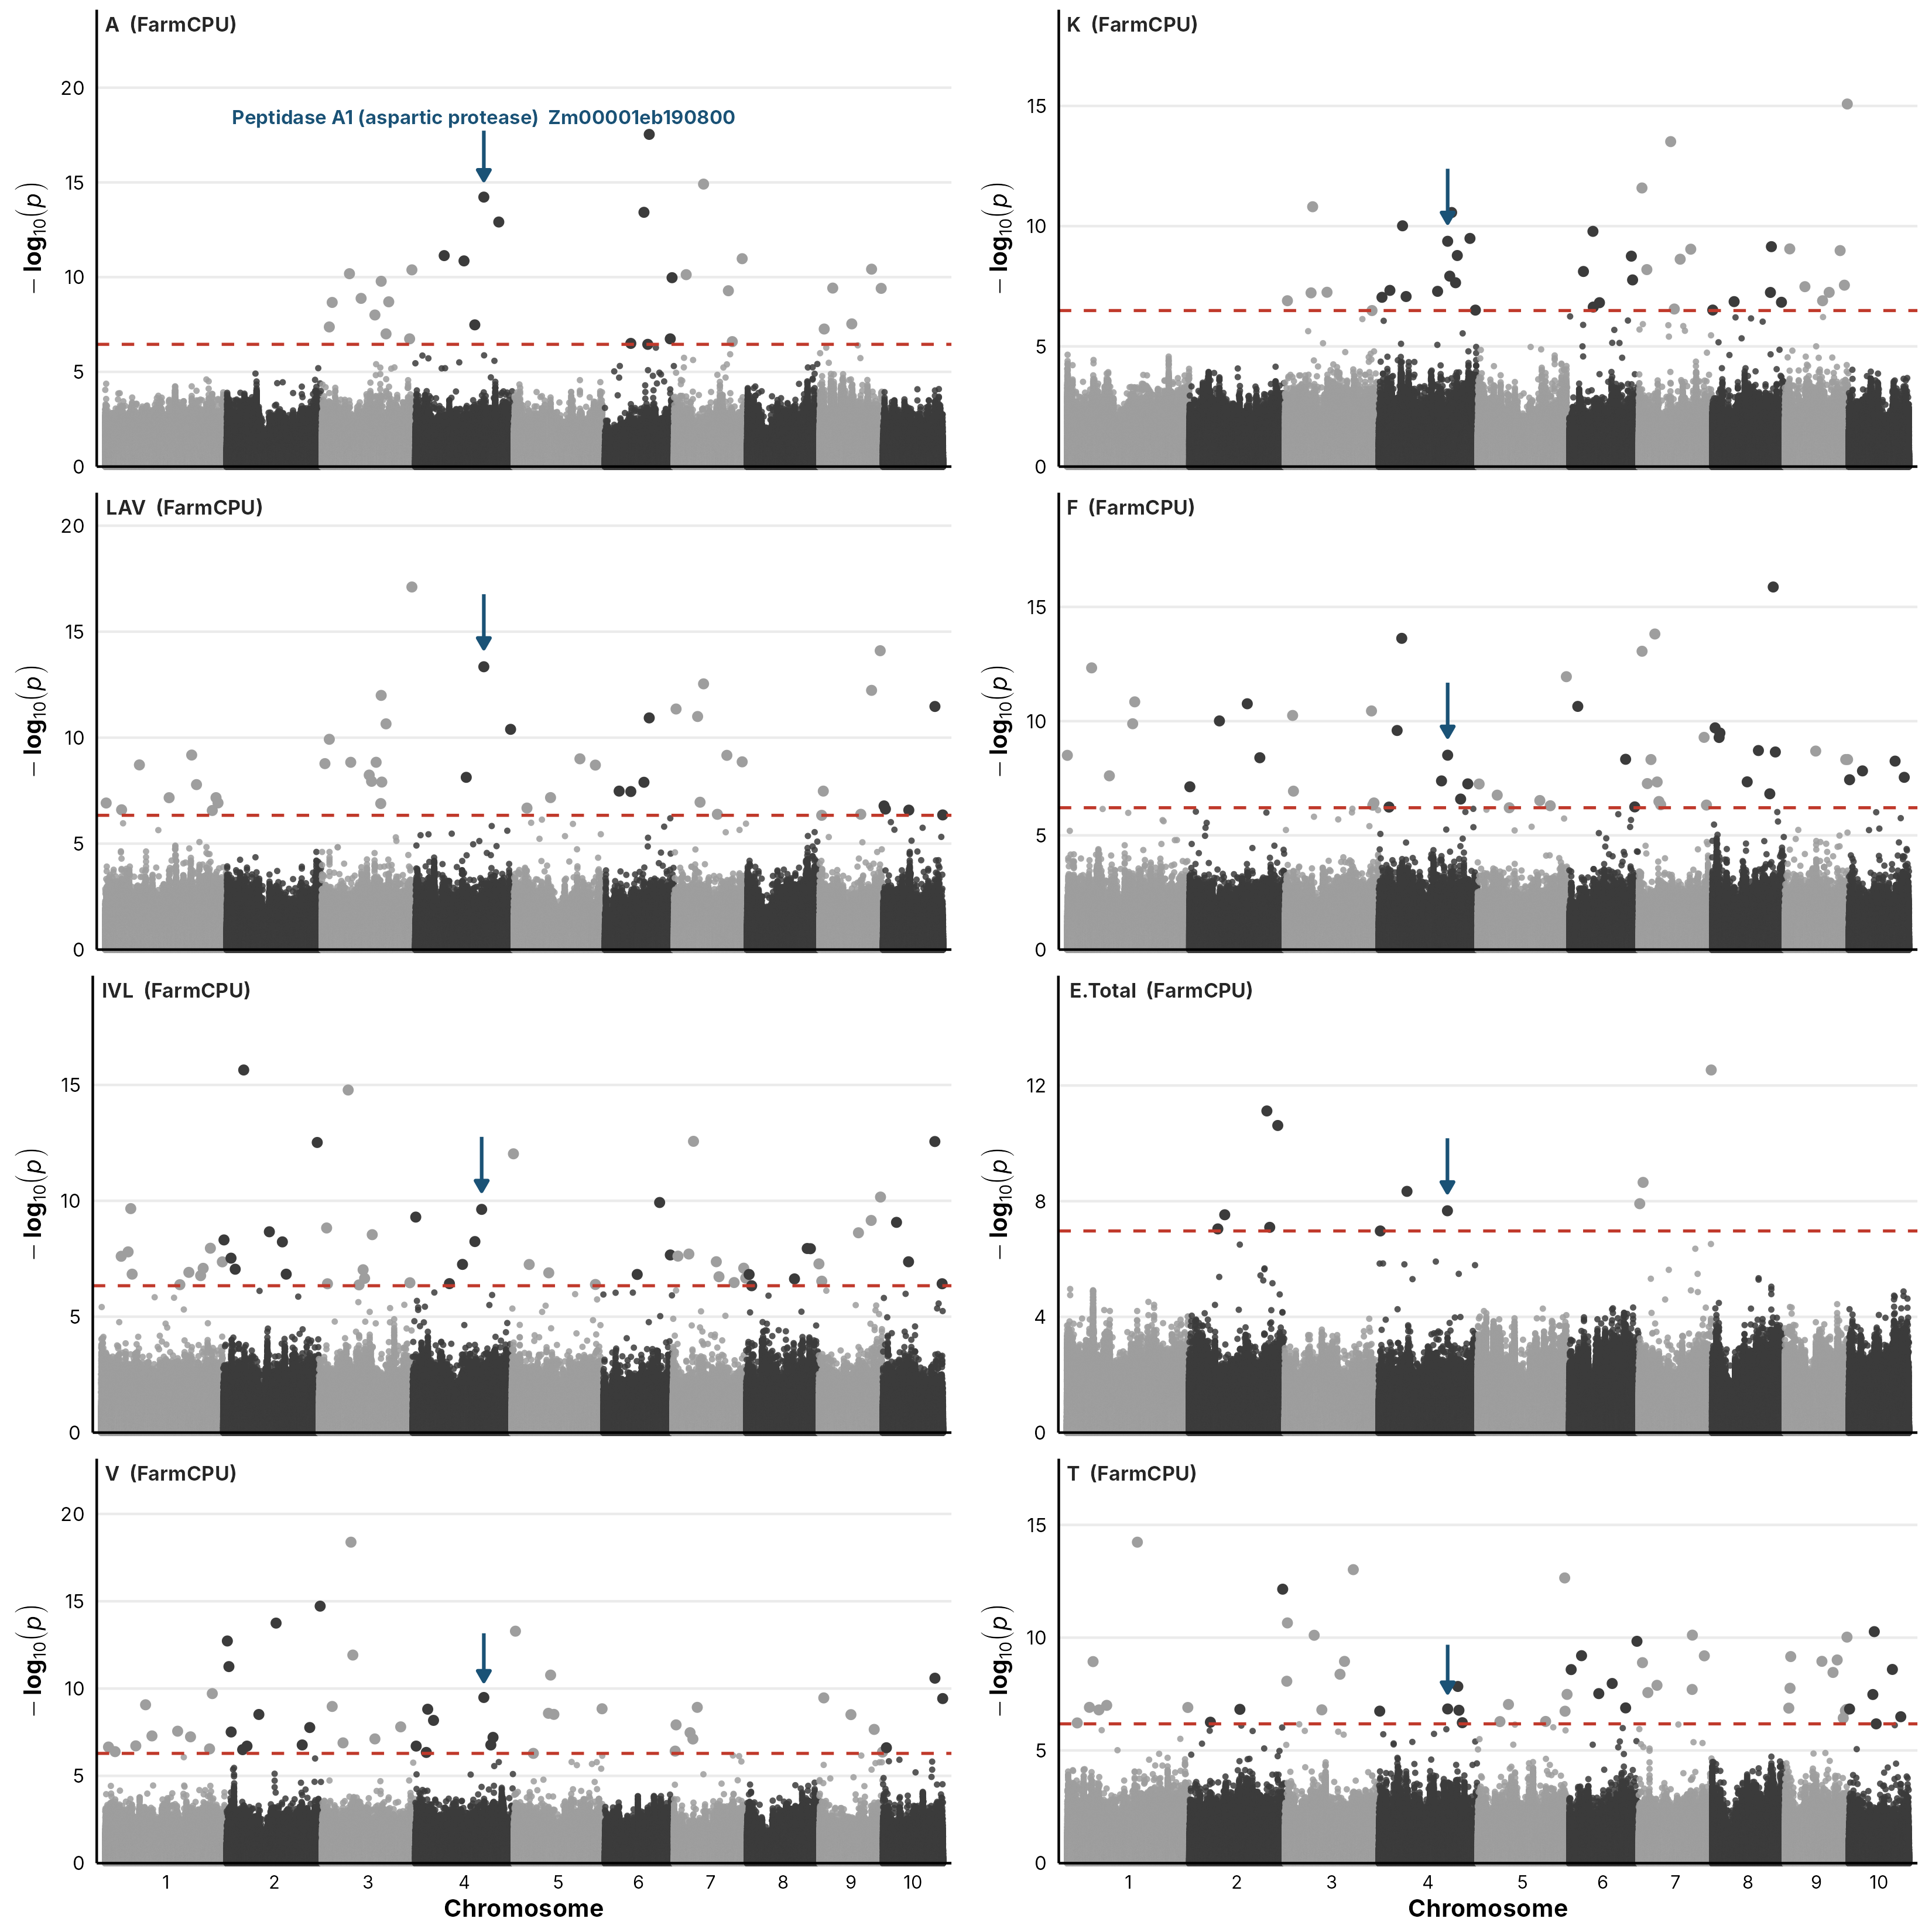
\includegraphics[width=0.82\textwidth]{final/main_figs/Fig_amino_chr4_peptidaseA1_manhattan.png}
    \caption{\textbf{Manhattan plots associated with eight amino acid traits link to an aspartic protease gene} A chromosome 4 locus associated with alanine (\textit{A}), \textit{LAV}, \textit{IVL}, valine (\textit{V}), lysine (\textit{K}), phenylalanine (\textit{F}), \textit{E.Total}, and threonine (\textit{T}) lies adjacent to a peptidase A1 (aspartic protease) gene. FarmCPU Manhattan plots show the significant traits at chr4:174.55–174.57 Mb. Arrows indicate the top SNP within \textit{Zm00001eb190800}. Red dashed lines mark the 5\% Benjamini–Hochberg FDR thresholds.}
    \label{fig:amino_locus_manhattan}
\end{figure*}

\subsection{Association mapping identifies amino acid metabolism and transport candidates for abundant, heritable free amino acids}

To identify loci affecting grain amino acid composition, we defined 78 amino acid–derived phenotypes (Supplementary Tables S1--S2), including the absolute abundance of 20 individual FAAs; six biosynthetic-family composites (IMNTDK, EHPRQ, SGC, WFY, LAV, IVL); 20 ratios to the total free pool; 25 ratios to the family composite; four ratios between amino acids (N.D, N.E, N.Q, Q.E); and three whole-pool measures (total FAA, total PBAA \citep{Shrestha2022}, and estimated nitrogen).

We ran GWAS using three models (MLM, BLINK, and FarmCPU). At a BH FDR of 5\%, we found 2,461 significant SNPs across 71 phenotypes, forming 2,152 loci and yielding 3,693 candidate genes (Supplementary Tables S6--S7). Most candidate genes were specific to one phenotype (3,002), 691 were shared by two or more phenotypes, and only 193 by more than two. The number of candidate genes per phenotype was similar across biosynthetic families (71, 69, and 67 for Asp-, Glu-, and Ser-family phenotypes), so families with more phenotypes simply had more candidate genes. The loci associated with the most phenotypes were not near amino acid biosynthesis genes. Three loci were each associated with nine phenotypes. The locus on chromosome 4 (212.55 Mb) had no gene within 25 kb, and the locus on chromosome 7 (40.80 Mb) was near a K homology domain protein gene (\textit{Zm00001eb306240}). The locus on chromosome 9 (133.93 Mb) contained four genes, including an ER membrane protein complex subunit 4 gene (\textit{Zm00001eb394360}) and a rhomboid-like protein gene (\textit{Zm00001eb394380}), but its nine phenotypes were explained by only three groups of SNPs (Supplementary Fig.~\ref{fig:supp_amino_chr9_locus}), because many phenotypes are ratios or composites of the same amino acids. A fourth locus on chromosome 4 at 174.57 Mb was associated with eight phenotypes from four biosynthetic families (\textit{A}, \textit{V}, \textit{K}, \textit{F}, \textit{T}, \textit{LAV}, \textit{IVL}, and \textit{E.Total}), with significant SNPs 2.6--6.1~kb upstream and 5.9~kb downstream of a peptidase A1 (aspartic protease) gene (\textit{Zm00001eb190800}; Fig.~\ref{fig:amino_locus_manhattan}).

Furthermore, we investigated individual FAAs (Table~\ref{tab:amino_gwas_focus}). Asn, the most abundant ($H^2=0.83$, $h^2_g=0.68$), had the most loci (356 across abundance and five ratios) and candidates, including two asparagine synthetase domain genes (\textit{Zm00001eb036060}, \textit{Zm00001eb036070}; \textit{N.E}), a glutamine amidotransferase type 2 (\textit{Zm00001eb329710}; \textit{N.E}, $P=6.1\times10^{-10}$), homoserine dehydrogenase (\textit{Zm00001eb405410}; \textit{N.IMNTDK}, SNP within gene), and lysine-branch enzymes dihydrodipicolinate synthase/reductase (\textit{Zm00001eb389290}, \textit{Zm00001eb176170}). An AVT6C transporter (\textit{Zm00001eb368680}) was significant for Asn ($P=1.3\times10^{-8}$) and the Asp-family composite ($P=2.5\times10^{-11}$) in both BLINK and FarmCPU. For lysine, the most heritable FAA ($H^2 = 0.88$, $h^2_g = 0.73$), a SNP for lysine as a fraction of the total free pool (\textit{K.Total}; $P = 2.5 \times 10^{-11}$; significant in BLINK and FarmCPU) lies in \textit{Zm00001eb277160}, an NRT1/PTR family 4.6 transporter gene. Another SNP for lysine relative to aspartate-family amino acids (\textit{K.IMNTDK}; $P = 2.8 \times 10^{-11}$) is 15~kb from \textit{Zm00001eb360480}, which encodes NADH-dependent glutamate synthase.

Pro, the second most abundant FAA, was nearly as heritable as Asn ($H^2 = 0.80$), but it had a lower genomic heritability ($h^2_g = 0.40$), suggesting that the markers capture less of its variation among lines. It also had fewer loci (59). However, its ratio traits had no significant associations. One proline SNP lies within a class I glutamine amidotransferase gene (\textit{Zm00001eb217220}; $P = 2.2 \times 10^{-9}$). Glutamine, the second most variable FAA (CV 130\%) with high genomic heritability (0.85), showed the strongest association among the amino acids in Table~\ref{tab:amino_gwas_focus} ($P = 4.9 \times 10^{-22}$, \textit{Q.E}). A SNP for free glutamine (\textit{Q}; $P = 1.2 \times 10^{-11}$) lies within a WAT1-related (UmamiT) gene on chromosome 9 (\textit{Zm00001eb379220}). A SNP for the Gln/Glu ratio (\textit{Q.E}; $P = 8.4 \times 10^{-8}$) lies within the amino acid/auxin permease gene \textit{aaap40} (\textit{Zm00001eb261470}) on chromosome 6, in a 240-kb region that also contains the lysine histidine transporters \textit{LHT1} (\textit{Zm00001eb261480}) and \textit{LHT2} (\textit{Zm00001eb261440}) and three further amino acid permeases (\textit{aaap41}, \textit{aaap43}, \textit{aaap44}; \textit{Zm00001eb261490}--\textit{Zm00001eb261510}). Methionine, the most variable FAA (CV 180\%), had 104 loci but no trait-matched candidate gene. Its high CV likely reflects a strongly skewed distribution across lines, where the highest line had about 200 times as much Met as the lowest (Supplementary Table S3). Thus, genes involved in Asn/Asp-family metabolism and amino acid transport linked to their respective amino acids, whereas loci common to multiple phenotypes suggested roles in protein turnover rather than in single biosynthetic reactions.

To test whether the free Asp and Pro variation seen in the panel also segregates in a biparental cross, we mapped both traits in a B64 $\times$ CML14 F$_{2:3}$ population developed to map kernel free Asn, in which Asn is controlled mainly by a single QTL at \textit{ASN3} on chromosome~1 \citep{Fitzsimmons2026KernelKitchen}. Because B64 and CML14 were chosen for Asn rather than Asp or Pro, this analysis was exploratory. In the Goodman--Buckler panel, CML14 was among the lowest lines for free Asp, and B64 was near the median, with both being below the median for Pro (Supplementary Fig.~\ref{suppfig:qtl_asp_pro}A,C). We identified a single QTL for each trait at the same position on chromosome 3 (peak at 35.99~Mb), with LOD 6.12 for Asp (threshold 3.70, 1,000 permutations) and 4.55 for Pro (threshold 3.63), explaining 10\% and 7\% of phenotypic variance, respectively (Supplementary Fig.~\ref{suppfig:qtl_asp_pro}B,D). This shared QTL was distinct from the Asn QTL, indicating that free Asp and Pro share genetic control that is separable from Asn in this cross. The 1.5-LOD support intervals for this shared peak were similar in size and location, spanning 14.25 and 15.27 cM for Pro and Asp, respectively, and contained 1,550 and 1,578 genes (Supplementary Table S8). The interval spans the low-recombination region around the chromosome 3 centromere, so it cannot resolve a causal gene. However, within 1.5 cM of the peak, it includes the tandem pair of CC-type glutaredoxin genes (\textit{Zm00001eb131830}, \textit{Zm00001eb131840}) and the LHT-like amino acid transporter (\textit{Zm00001eb132750}), all of which also lie in highly differentiated Jarvis windows (see below). Of these, only the LHT-like gene is consistently expressed in developing kernels (Supplementary Table S8).

%===================== TABLE 1 =====================

\begin{table*}[t]
\centering
\caption{\textbf{Association mapping of the focal FAAs in the Goodman--Buckler panel.} Median, coefficient of variation (CV), line-mean broad-sense heritability ($H^2$) and genomic heritability ($h^2_g$) are from Supplementary Table~S3. Loci: loci (Supplementary Table~S7) significant at 5\% Benjamini--Hochberg FDR for at least one phenotype reporting on the amino acid; in parentheses, loci for the absolute trait alone. Best $P$: smallest $P$ among those phenotypes. Trait-matched candidate genes: genes within 25 kb of a significant SNP with their putative function.}
\label{tab:amino_gwas_focus}
\footnotesize
\setlength{\tabcolsep}{3pt}
\begin{tabularx}{\textwidth}{@{}l r r r r r r >{\raggedright\arraybackslash}X@{}}
\hline
FAA & Median & CV (\%) & $H^2$ & $h^2_g$ & Loci & Best $P$ & Trait-matched candidate genes (putative function) \\
\hline
Asparagine (N) & 3.783 & 70 & 0.83 & 0.68 & 356 (73) & $2.8\times10^{-20}$ & \textit{Zm00001eb368680} (amino acid transporter AVT6C); \textit{Zm00001eb329710} (glutamine amidotransferase type 2); \textit{Zm00001eb405410} (homoserine dehydrogenase); \textit{Zm00001eb036060} (asparagine synthetase domain); \textit{Zm00001eb036070} (asparagine synthetase domain); \textit{Zm00001eb389290} (dihydrodipicolinate synthase); \textit{Zm00001eb176170} (dihydrodipicolinate reductase) \\
Proline (P) & 3.202 & 63 & 0.80 & 0.40 & 59 (59) & $2.7\times10^{-15}$ & \textit{Zm00001eb217220} (glutamine amidotransferase) \\
Lysine (K) & 0.272 & 90 & 0.88 & 0.73 & 116 (54) & $8.3\times10^{-16}$ & \textit{Zm00001eb277160} (NRT1/PTR family 4.6); \textit{Zm00001eb360480} (glutamate synthase (NADH)); \textit{Zm00001eb352400} (WAT1-related (UmamiT)) \\
Aspartate (D) & 1.178 & 76 & 0.81 & 0.84 & 91 (20) & $3.3\times10^{-16}$ & \textit{Zm00001eb207630} (WAT1-related (UmamiT)) \\
Glutamine (Q) & 0.371 & 130 & 0.69 & 0.85 & 165 (65) & $4.9\times10^{-22}$ & \textit{Zm00001eb379220} (WAT1-related (UmamiT)); \textit{Zm00001eb261470} (amino acid transporter); \textit{Zm00001eb261480} (amino acid transporter); \textit{Zm00001eb261490} (amino acid transporter) \\
Methionine (M) & 0.047 & 180 & 0.78 & 0.46 & 104 (56) & $3.2\times10^{-17}$ & none \\
\hline
\end{tabularx}
\end{table*}

\subsection{Soil nitrogen environment GWAS of maize landraces points to candidate genes in aspartate-family and amide nitrogen metabolism}

In the Goodman--Buckler panel, the free amino acid pool of the grain was dominated by Asn and Pro, which, along with Lys and Asp, were also among the most heritable free amino acids. Association mapping identified 3,693 candidate genes, including genes involved in Asn and Asp-family metabolism and amino acid transport. Because amino acids are the main transport form of nitrogen in the plant, their metabolism may also respond to nitrogen availability in the soil. However, these inbred lines represent standing variation in temperate germplasm grown under managed fertility. We therefore turned to maize landraces collected across a soil nitrogen gradient (Fig.~\ref{fig:soilN_gwas}B) and asked whether genetic variation associated with soil N implicates similar nitrogen-metabolism functions. Because soil N reflects the historical collection environment rather than a grain phenotype, we did not equate soil N adaptation with grain amino acid composition.

We associated the georeferenced maize landrace panel \citep{RomeroNavarro2017Landraces} with soil N at each collection site \citep{Poggio2021SoilGrids}, using 0--5 cm as the primary phenotype and 5--15 cm for validation (highly correlated; $r = 0.84$ across 3,107 accessions; Fig.~\ref{fig:soilN_gwas}A--B). Soil N is a property of the collection site, so accessions from the same or nearby sites share both soil N values (467 distinct values among 3,107 accessions) and ancestry. As a result, genomic heritability was $\sim$1.00 and remained 0.98 after removing 50 genotype PCs (permuted $h^2 \le 0.05$; Fig.~\ref{fig:soilN_gwas}C), reflecting shared ancestry and location rather than heritable variation in the plants. We therefore tested for confounding by relatedness and geography directly. Similarly, across three GWAS (MLM, BLINK, FarmCPU) models, 234 SNPs were significant at 5\% FDR (Fig.~\ref{fig:soilN_gwas}D). BLINK detected 218, FarmCPU 30, and MLM 2. Most SNPs were detected by a single model (203 by BLINK and 16 by FarmCPU), and 15 were detected by at least two, 13 by BLINK and FarmCPU, one by MLM and BLINK, and one (S5\_22338979) by all three. In total, 448 genes lie within 25~kb of 216 of these SNPs (Supplementary Table S9).

Because soil N varies across the landscape and landrace ancestry follows geography, an association with soil N can arise from shared ancestry or from other site variables that covary with soil N, rather than from soil N itself. We therefore filtered the soil N SNPs in several steps, using two tests to assess whether associations reflected soil N rather than geography or climate, and then focusing on SNPs detected by more than one model. The first asked whether the same SNPs were detected when other site variables were used as the GWAS phenotype. We ran GWAS with the same models for latitude, longitude, elevation, soil pH, CEC, and aridity and counted SNPs shared with soil N (Supplementary Fig.~\ref{suppfig:soilN_specificity}; Supplementary Tables S10--S11). Only 2 of the 234 soil-N SNPs were also significant for latitude, longitude, or elevation, close to the 0.7 expected by chance ($P = 0.14$). By contrast, soil N shared many SNPs with aridity (38 compared to 0.2 expected) and soil pH (13 compared to 0.1), which covary with it. In total, 190 of the 234 SNPs were not significant for any other variable. Because a SNP can follow a geographic gradient without reaching significance in another GWAS, the second test did not use a GWAS model. For every SNP in the genome, we calculated the correlation between genotype and each site variable across the 3,107 accessions and considered a soil N SNP linked to another variable if its correlation was in the top 1\% of the genome for that variable (Supplementary Fig.~\ref{suppfig:soilN_geno_env}; Supplementary Tables S12--S13). By this measure, 13.2\% of soil N GWAS SNPs were linked to a geographic variable, compared with 1.8\% of all SNPs and 35.9\% of SNPs selected only for their correlation with soil N ($P = 5.9 \times 10^{-15}$). The GWAS models therefore removed much, but not all, of the geographic signal. Overall, 168 of the 234 SNPs passed both tests. Because associations detected by a single model are less reliable, we focused on the 15 SNPs detected by at least two models. Of these, 14 passed the first test and 12 passed both (Table~\ref{tab:soilN_specific}). The three that failed included the strongest signal (S9\_151742636; $P = 2.6 \times 10^{-13}$), which was also significant for aridity and soil pH. Of the 12, five had genotypes correlated with soil N but not with other site variables. The other seven had genotypes only weakly correlated with soil N itself, so the lack of correlation with other variables was uninformative for them.

Four soil N SNPs map near genes involved in Asp-family or amide nitrogen metabolism. S5\_22338979 lies 4.4 kb upstream of \textit{Zm00001eb220040}, an amino acid kinase-domain gene annotated with aspartate kinase activity, the first step of the aspartate-derived amino acid pathway. It is the only soil-N SNP significant in all three models and is also significant at 5--15 cm. S1\_16128632 lies within \textit{Zm00001eb005710}, an $\omega$-amidase/NIT2-like CN-hydrolase \citep{Zhang2014OmegaAmidase}. Both SNPs are rare (minor allele frequencies of 0.030 and 0.016), so their associations rest on few accessions. Because both SNPs are rare, we examined where the minor-allele carriers were collected (Supplementary Fig.~\ref{suppfig:soilN_focal_geography}). Carriers of the $\omega$-amidase allele came from 56 collection sites, and carriers of the aspartate kinase allele came from 115 sites, each spanning 11 countries, so neither association rests on a single site or local population. Both alleles were concentrated in Mexico and Central America (87\% and 93\% of carriers, compared with 74\% of the panel) and were nearly absent from South America (5 of 667 accessions for each allele). Carriers came from soils with more N than non-carriers (median 414 compared with 251 for $\omega$-amidase and 356 compared with 248 for aspartate kinase), and both heterozygous and homozygous carriers showed this shift (Kruskal--Wallis $P = 4.4 \times 10^{-9}$ and $3.3 \times 10^{-10}$). Because soil N also differs between regions, we compared carriers with non-carriers within regions. Within Mexico, $\omega$-amidase carriers came from soils with nearly twice the N of non-carriers (median 424 compared with 233, 28 carriers, Wilcoxon $P = 1.0 \times 10^{-4}$), whereas the difference within Central America was smaller (451 compared with 404, 25 carriers, $P = 0.32$). For aspartate kinase, the differences within Mexico (268 compared with 232, 75 carriers, $P = 6.4 \times 10^{-4}$) and within Central America (445 compared with 403, 39 carriers, $P = 0.06$) were smaller, indicating that part of its overall association reflects the higher soil N of Central America, where the allele is more common, although carriers still came from N-richer soils within Mexico. Thus, the minor alleles at both loci are more frequent at N-rich collection sites, most clearly for $\omega$-amidase within Mexico, although the regional concentration of carriers means that shared ancestry cannot be excluded. S8\_138640842, the strongest of the 12 SNPs that passed both tests ($P = 3.5\times10^{-11}$), lies within \textit{Zm00001eb356170} (methionine S-methyltransferase). However, it was supported only by BLINK and FarmCPU and was inconclusive in the correlation test. At 5--15 cm, S8\_133179205 lies 0.1~kb from \textit{Zm00001eb354640} (S-adenosylmethionine synthase) and was not linked to other site variables. The same gene was a candidate in the grain amino acid GWAS (\textit{I.IVL}; $P = 1.0 \times 10^{-8}$). Thus, the soil-N GWAS in landraces, like the grain amino acid GWAS, points to Asp-family and amide nitrogen metabolism.

%===================== TABLE 2 =====================
\begin{table*}[ht]
  \centering
  \scriptsize
  \caption{\textbf{Soil-N SNPs detected by at least two GWAS models that passed both environmental specificity tests.} SNPs were FDR-significant (5\%) for soil N at 0--5~cm in at least two of MLM (M), BLINK (B) and FarmCPU (F). They were not significant in the GWAS of latitude, longitude, elevation, soil pH, CEC or aridity (Supplementary Table~S11), and their genotype was not in the top 1\% of the genome for correlation with any of those variables (Supplementary Table~S12). $P$, lowest $P$ across models. 5--15~cm, also FDR-significant for soil N at 5--15~cm. Corr., genotype--environment call, either not linked (genotype in the top 5\% for correlation with soil N and not in the top 1\% for any other variable) or inconclusive (genotype outside the top 5\% for correlation with soil N, so the association is detected only by the multi-locus models). Gene (distance), gene within 25~kb of the SNP and its distance, or within if the SNP lies in the gene.}
  \label{tab:soilN_specific}
  \begin{tabular}{llrlrrllll}
  \hline
  SNP & Chr & Position & Models & MAF & $P$ & 5--15 cm & Corr. & Gene (distance) & Annotation \\
  \hline
  S8\_138640842 & 8 & 138,640,842 & BF  & 0.254 & $3.5\times10^{-11}$ & no  & inconclusive & \textit{Zm00001eb356170} (within) & Methionine S-methyltransferase \\
  S1\_87643408  & 1 &  87,643,408 & BF  & 0.356 & $2.6\times10^{-10}$ & no  & inconclusive & \textit{Zm00001eb022740} (within) & Syndetin \\
  S2\_191754648 & 2 & 191,754,648 & BF  & 0.074 & $6.2\times10^{-10}$ & no  & inconclusive & \textit{Zm00001eb100890} (within) & Uncharacterized protein \\
  S5\_22338979  & 5 &  22,338,979 & MBF & 0.030 & $1.9\times10^{-8}$  & yes & not linked   & \textit{Zm00001eb220040} (4.4 kb) & Amino acid kinase domain \\
  S8\_153826994 & 8 & 153,826,994 & BF  & 0.020 & $5.1\times10^{-8}$  & no  & inconclusive & \textit{Zm00001eb359990} (within) & Homeobox-DDT protein RLT1 \\
  S3\_54622531  & 3 &  54,622,531 & BF  & 0.050 & $6.5\times10^{-8}$  & yes & not linked   & \textit{Zm00001eb130210} (17.9 kb) & RING/FYVE/PHD zinc finger (TTL1-like) \\
  S5\_22338938  & 5 &  22,338,938 & MB  & 0.031 & $6.5\times10^{-8}$  & no  & not linked   & \textit{Zm00001eb220040} (4.3 kb) & Amino acid kinase domain \\
  S1\_16128632  & 1 &  16,128,632 & BF  & 0.016 & $2.9\times10^{-7}$  & no  & not linked   & \textit{Zm00001eb005710} (within) & $\omega$-amidase/NIT2-like CN-hydrolase \\
  S5\_53136163  & 5 &  53,136,163 & BF  & 0.221 & $5.7\times10^{-7}$  & yes & inconclusive & \textit{Zm00001eb226000} (within) & Protein kinase \\
  S6\_37926580  & 6 &  37,926,580 & BF  & 0.179 & $7.4\times10^{-7}$  & no  & inconclusive & \textit{Zm00001eb265710} (within) & HB transcription factor \\
  S1\_5543355   & 1 &   5,543,355 & BF  & 0.090 & $1.2\times10^{-6}$  & yes & inconclusive & \textit{Zm00001eb001920} (within) & Transcription repressor \\
  S2\_117202525 & 2 & 117,202,525 & BF  & 0.071 & $2.1\times10^{-6}$  & no  & not linked   & -- & No gene within 25 kb \\
  \hline
  \end{tabular}
\end{table*}

%===================== FIGURE 2 =====================
\begin{figure*}[ht!]
  \centering
  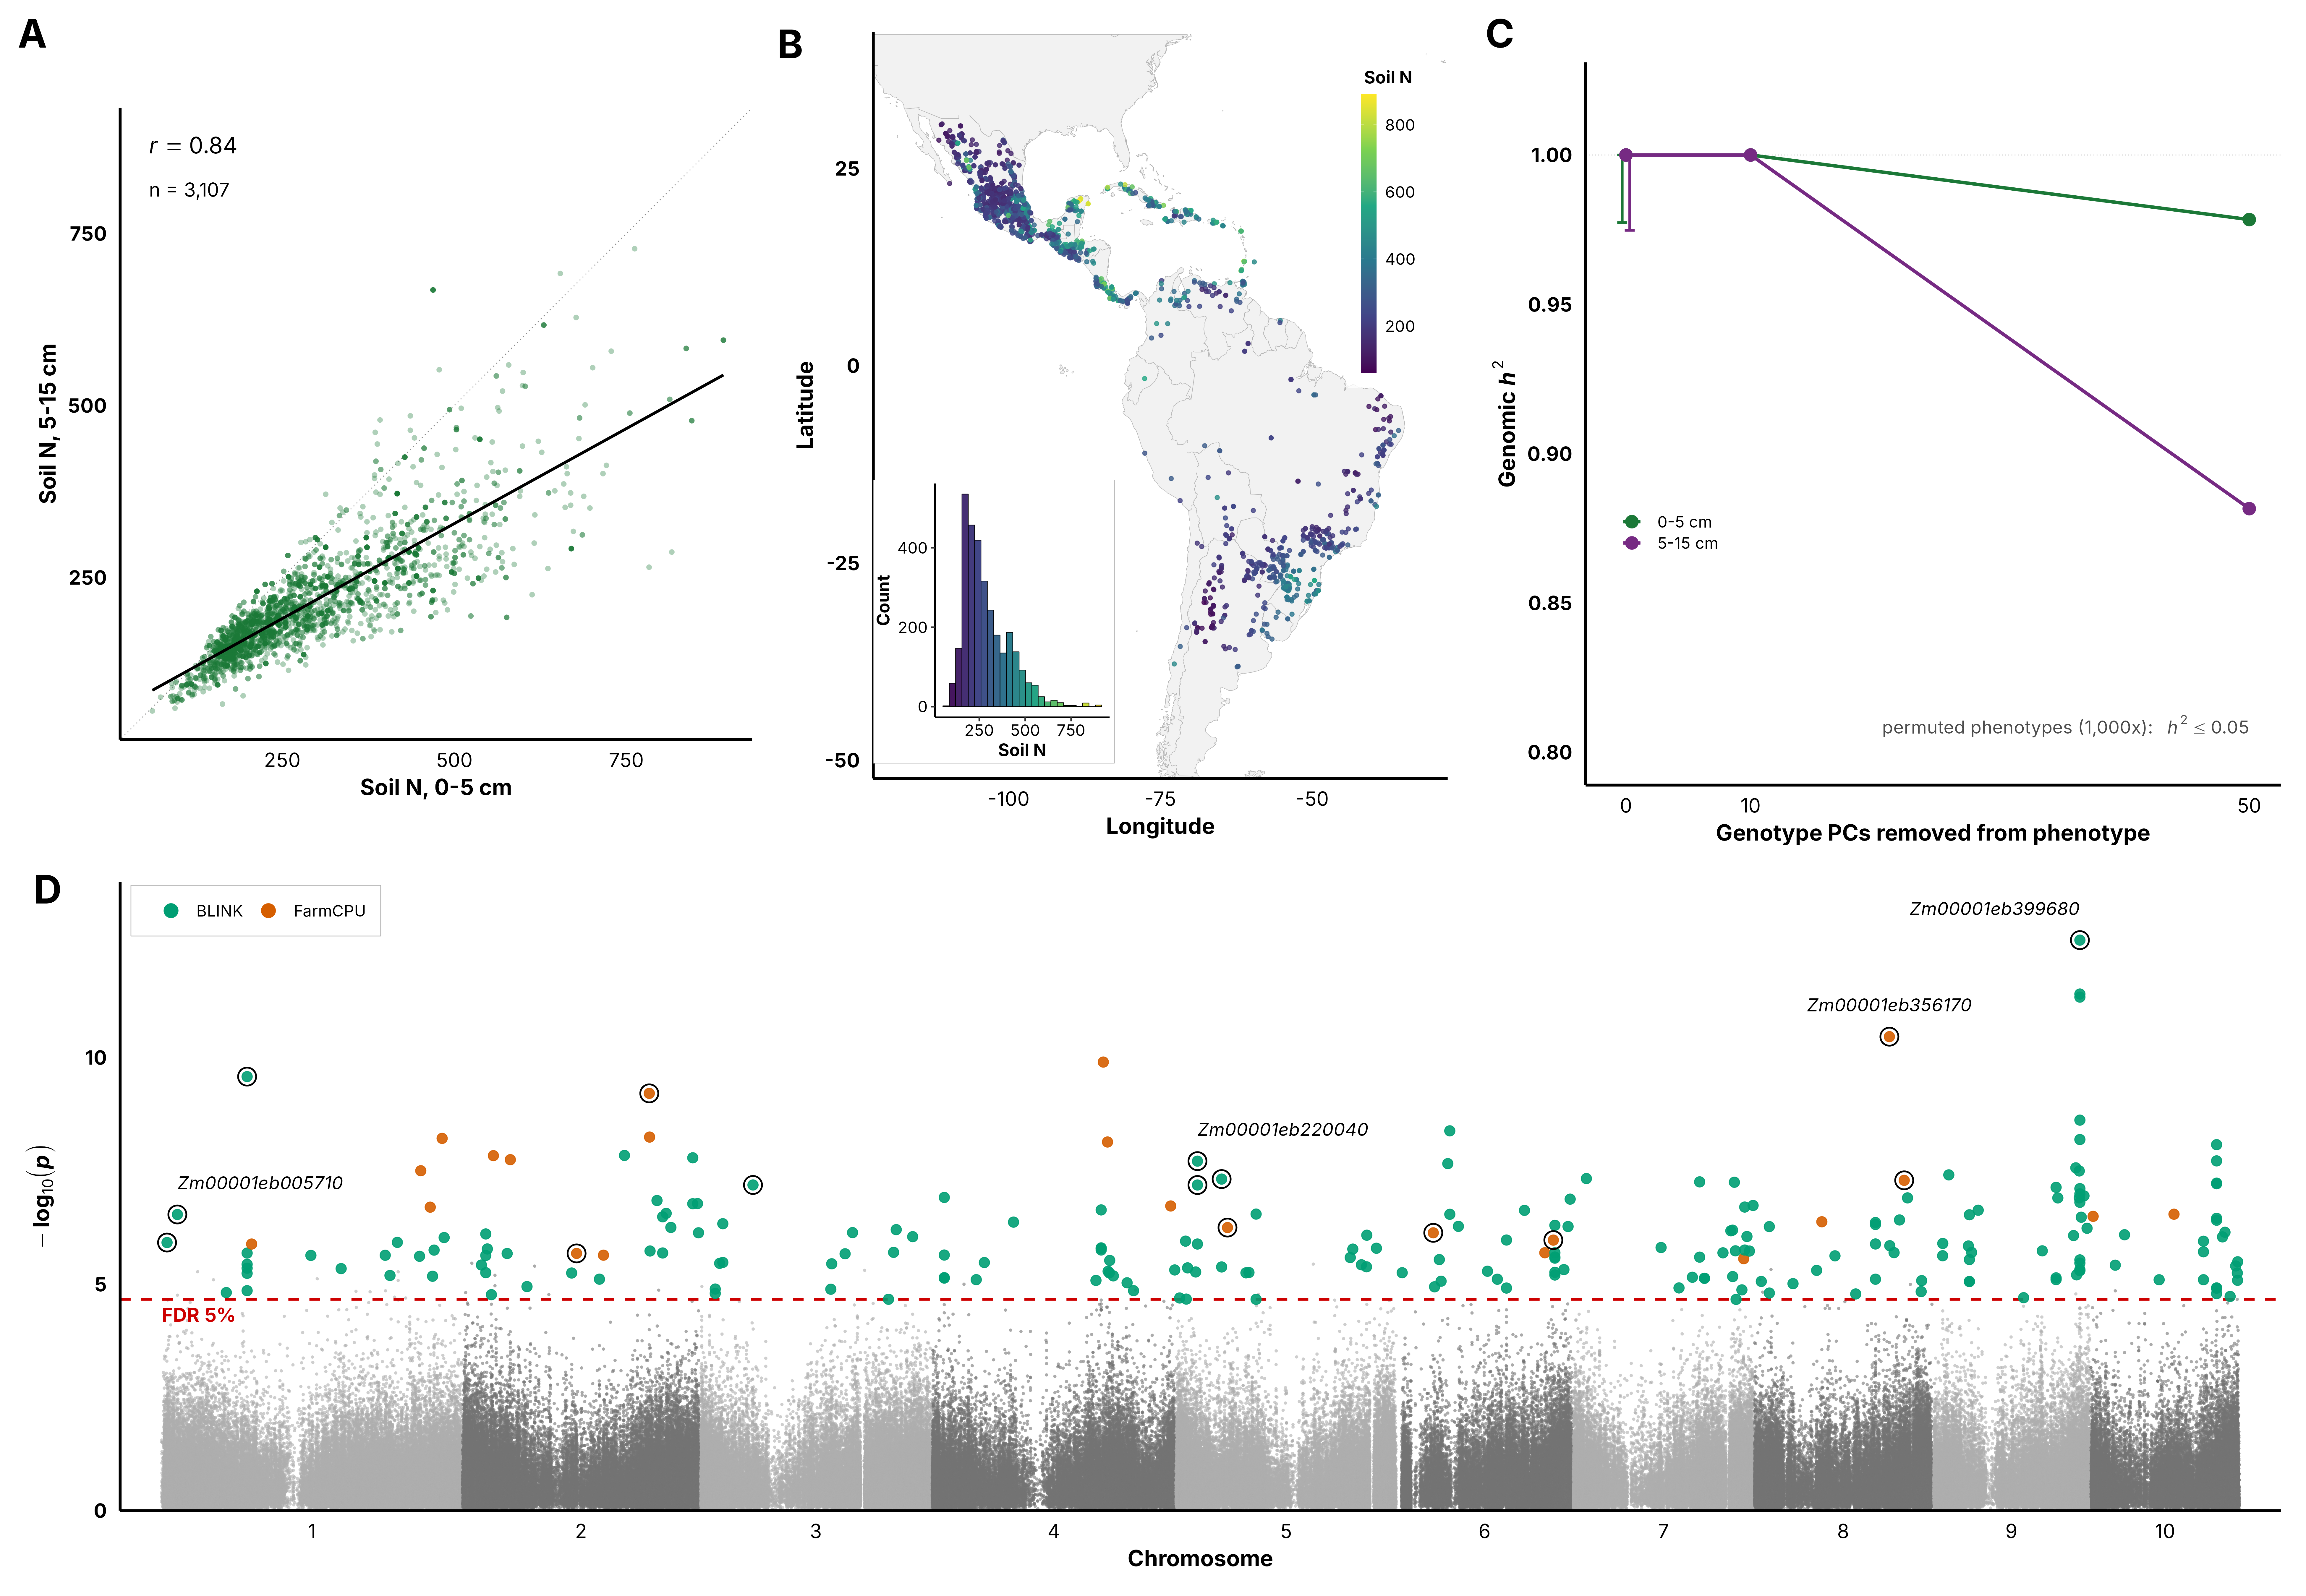
\includegraphics[width=\textwidth]{final/main_figs/Fig2_soilN.png}
  \caption{\textbf{Soil nitrogen at the collection site of 3,107 maize landraces.}
  \textbf{(A)} Soil N at 0--5\,cm vs.\ 5--15\,cm ($r = 0.84$); solid line, least-squares fit;
  dotted line, $y = x$.
  \textbf{(B)} Collection sites colored by soil N at 0--5\,cm; inset, distribution of
  soil N across accessions.
  \textbf{(C)} Genomic heritability ($h^2$) of soil N at both depths after removing
  0, 10 and 50 genotype principal components from the phenotype; error bars, 95\% CI at
  0 PCs; permuted phenotypes (1,000$\times$) gave $h^2 \leq 0.05$.
  \textbf{(D)} Manhattan plots for soil N (0--5\,cm); colored points are SNPs significant at 5\% Benjamini--Hochberg FDR in at least one model (MLM, BLINK, FarmCPU; 3 PCs), colored by the model with the lowest $P$; the SNPs near the aspartate kinase isozyme (\textit{Zm00001eb220040}) and the $\omega$-amidase (\textit{Zm00001eb005710}) are ringed and labeled. The dashed red line marks the 5\% FDR threshold. Candidate genes named in the text are labeled.}
  \label{fig:soilN_gwas}
\end{figure*}

\subsection{Free amino acid profiles of Indian Chief and Jarvis show population-specific remodeling of the soluble amino acid pool}

The Goodman--Buckler panel captured standing variation in grain amino acids, and landraces captured variation tied to natural soil N gradients, but neither shows how the grain amino acid pool responds to yield selection. The Indian Chief and Jarvis maize populations address this question. Both were base populations in a 14-cycle reciprocal recurrent-selection experiment for yield, and selection shifted N allocation differently in seeds and stover \citep{Moll1994}. Under nonlimiting N, Jarvis Cycle 14 increased grain N mainly via greater grain weight, driven largely by higher post-anthesis soil N uptake, with little change in apparent stover-to-grain N remobilization. Indian Chief Cycle 14 maintained more post-anthesis stover biomass, lost less stover N after anthesis, and did not significantly increase grain N \citep{Moll1994}. Thus, grain N gains can arise from improved soil N recovery or altered internal N allocation during grain filling \citep{Mueller2019NUE}. Because amino acids deliver N to the kernel, we asked whether yield selection also remodeled the grain free amino acid pool, and whether populations with different N responses changed differently. We therefore treat the Indian Chief and Jarvis amino acid profiles as evidence of changes in the grain amino acid pool, not of changes in N allocation or remobilization.

We compared total FAA, the fractions of Pro, Asn, Asp, Gln, and Glu in the free pool, the N-rich FAAs (Asn + Gln + Arg + Lys + His), and FAA-derived N between Cycle 0 and Cycle 14 within each population, correcting for these eight tests (Fig.~\ref{fig:ic_j_faa}; Supplementary Table~S14). We also tested all 20 FAA fractions and the protein-bound pool separately (Supplementary Tables~S15--S17). Indian Chief showed significant changes in total FAA and composition. Total FAA per mg increased from 1.40 (Cycle~0) to 2.46 (Cycle 14) (Wilcoxon $P = 0.0043$; BH $P = 0.017$; Fig.~\ref{fig:ic_j_faa}A), with no overlap between cycles, and FAA-derived N increased accordingly (1.75 to 2.99 per mg; BH $P = 0.017$). Pro increased from 0.320 to 0.519 of total FAA ($P = 0.016$; BH $P = 0.025$), whereas Asp decreased from 0.115 to 0.075 ($P = 0.016$; BH $P = 0.025$), and Glu from 0.140 to 0.062 ($P = 0.0068$; BH $P = 0.018$). Asn and Gln fractions were unchanged (Fig.~\ref{fig:ic_j_faa}B). When all 20 FAA fractions were tested together, Pro, Asp, Glu, Ile, and Val differed nominally ($P \le 0.016$), but none remained significant after correction across the 20 tests (BH $P = 0.063$; Supplementary Table S15).

Jarvis showed one nominal change, but the test was underpowered with only three Cycle 0 samples. The Asp fraction increased from 0.075 (Cycle~0) to 0.137 (Cycle~14; $P = 0.019$), but it was not significant after correction (BH-adjusted $P = 0.15$). Total FAA per mg, the Pro and Glu fractions, the N-rich FAA pool, and FAA-derived N did not differ between cycles (Supplementary Table S14). The lack of corrected differences in Jarvis may reflect limited sampling, a stable FAA pool, or both. A stable pool is also consistent with \citet{Moll1994}, in which the greater grain N of Jarvis Cycle 14 came mainly from greater grain weight and post-anthesis N uptake rather than from increased remobilization from the stover.

To test whether changes in the free pool extended to total grain amino acid N, we converted FAA and PBAA abundances to amino acid derived N per mg. Protein-bound composition did not change across cycles in either population (Supplementary Fig.~\ref{fig:supp_pbaa_profiles}; Supplementary Tables~S15--S16). In Indian Chief, FAA-derived N increased from 1.75 to 2.99 per mg, but PBAA-derived N was more than 100-fold larger (332 and 364 per mg) and did not change, nor did total amino acid derived N ($P = 0.42$ for both; Supplementary Fig.~\ref{fig:supp_ic_j_aa_n_pools}; Supplementary Table~S17). Because FAAs carry less than 1\% of grain amino acid N, the larger free pool in Cycle 14 did not measurably change grain amino acid N, consistent with unchanged grain N in Indian Chief \citep{Moll1994}. Jarvis showed no change in any amino acid derived N pool. Thus, after 14 cycles of selection, Indian Chief had a greater total FAA and a composition that shifted from Asp/Glu toward Pro, whereas Jarvis showed no significant change. The protein-bound pool, which contains most grain amino acid N, was unchanged in both populations. These population-specific responses are consistent with reported differences in N allocation \citep{Moll1994}.

\begin{figure*}[ht!]
\centering
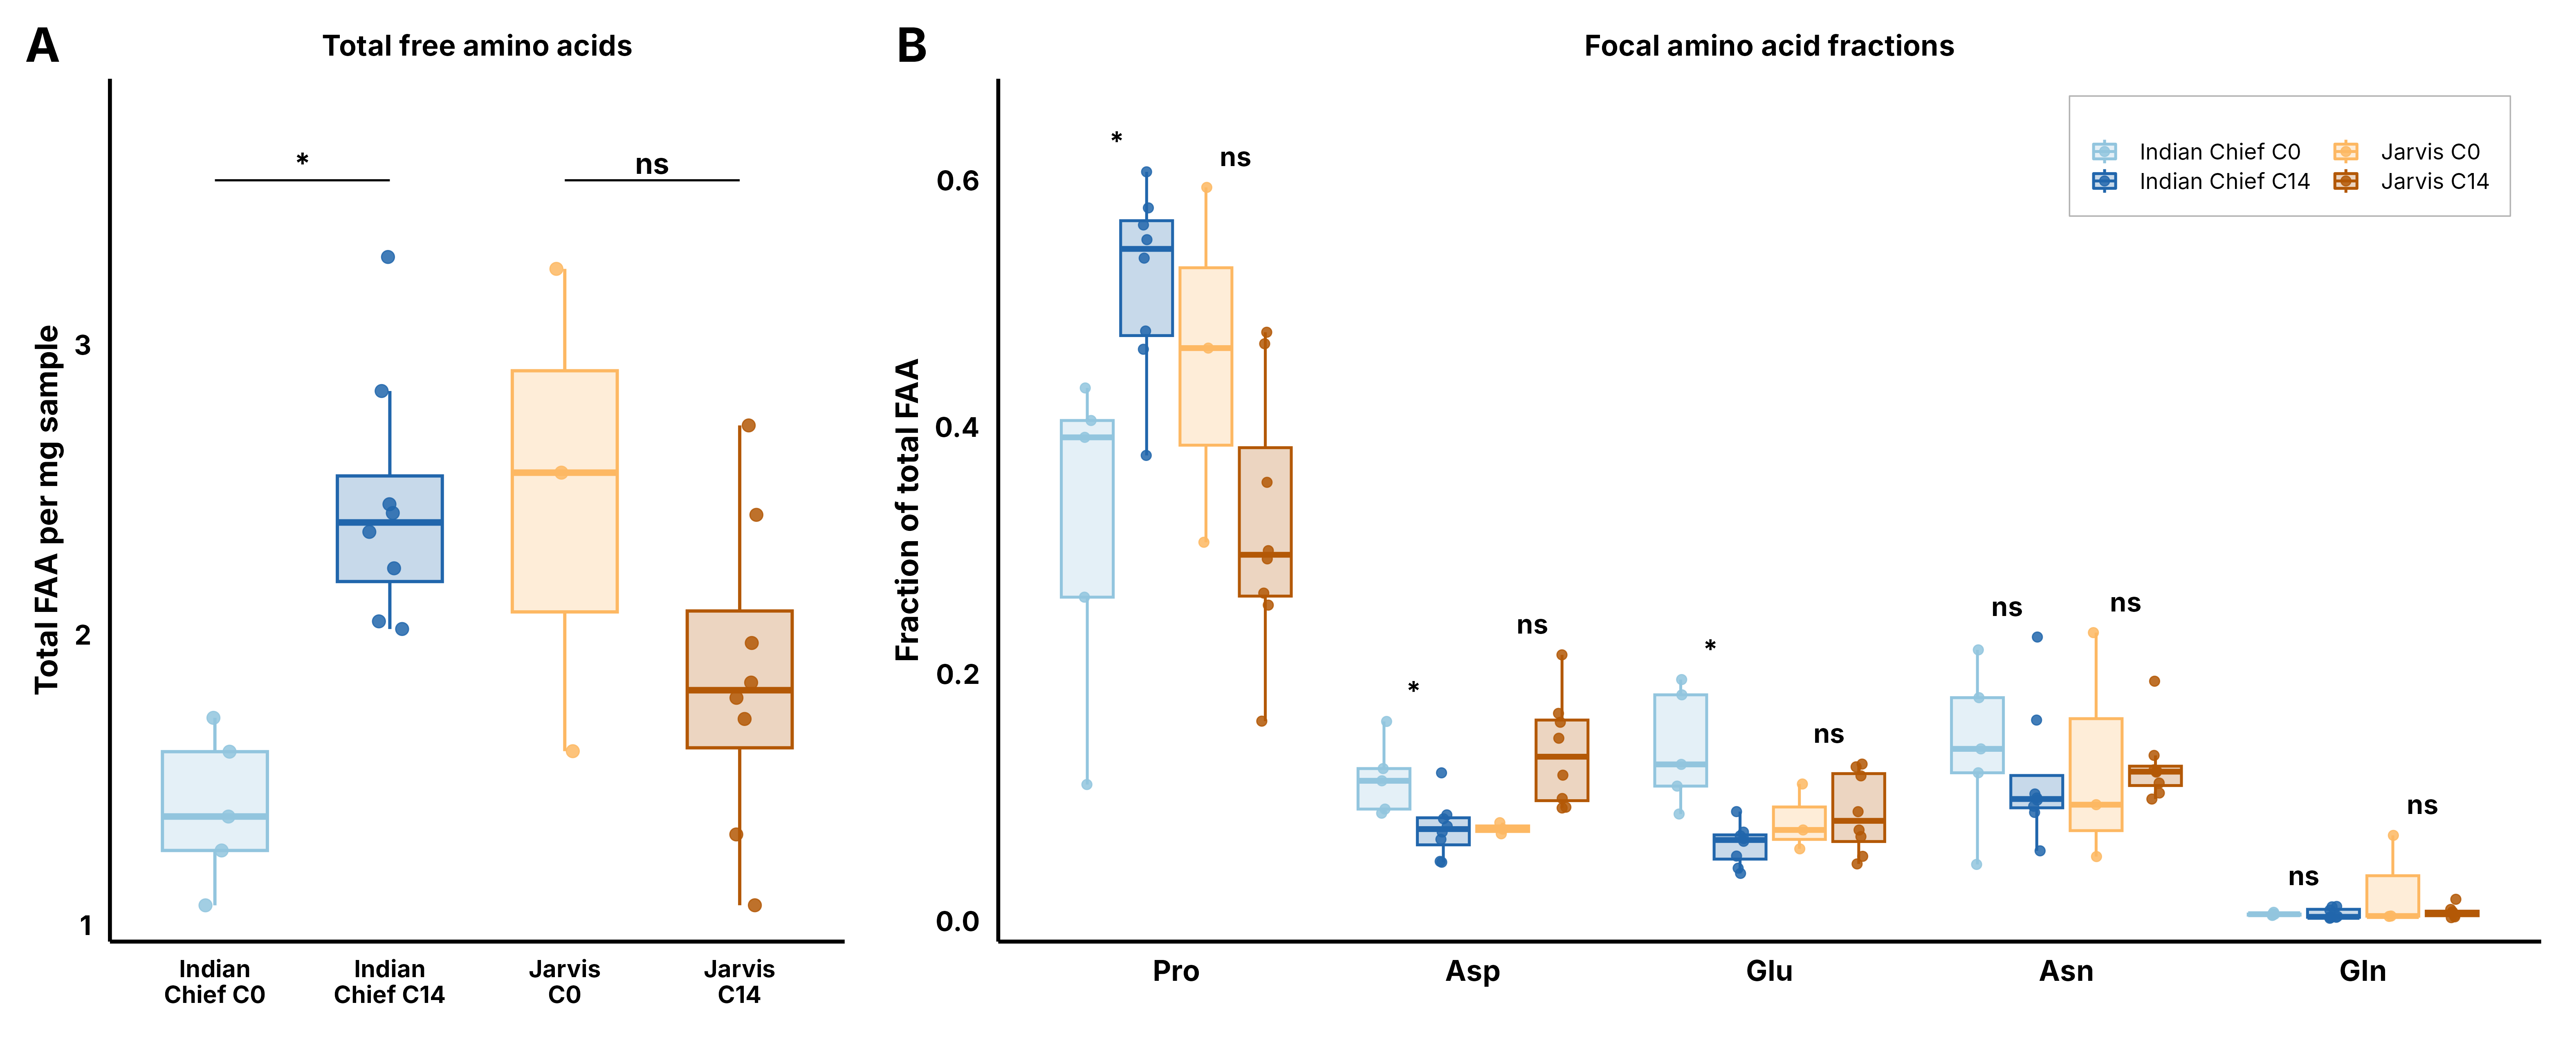
\includegraphics[width=\textwidth]{final/main_figs/Fig3_IC_J_FAA.png}
\caption{
\textbf{Free amino acid (FAA) pool and composition in Indian Chief and Jarvis before (C0) and after (C14) 14 cycles of reciprocal recurrent selection.} \textbf{(A)} Total FAA per mg sample. \textbf{(B)} Fractions of total FAA for Pro, Asp, Glu, Asn and Gln. Points are biological samples, each the mean of three technical replicates; boxes show the median and interquartile range. Within each population, C0 and C14 were compared with two-sided Wilcoxon rank-sum tests, and $P$ values were adjusted with the BH method; * adjusted $P < 0.05$; ns, not significant.
}
\label{fig:ic_j_faa}
\end{figure*}

\subsection{Skim sequencing reveals that Indian Chief and Jarvis diverged during reciprocal recurrent selection}

We skim sequenced 379 individuals from the Indian Chief and Jarvis populations at Cycle 0 and Cycle 14 (Indian Chief 96 and 92; Jarvis 96 and 95). The mean sequencing depth was 0.73$\times$ per individual and was higher at Cycle 14 than at Cycle 0 in both populations (Indian Chief 0.61$\times$ compared with 0.88$\times$; Jarvis 0.68$\times$ compared with 0.76$\times$; Supplementary Fig.~\ref{fig:supp_seq_sample}). At this depth, about half of the genotypes in each individual could not be called, and because the number of calls depends on depth, hard-called genotypes would differ between cycles for technical rather than biological reasons. We therefore used genotype likelihoods throughout, estimating population structure from 512,667 filtered SNPs (Supplementary Fig.~\ref{fig:supp_seq_variant}) and $F_{ST}$ directly from the aligned reads with ANGSD \citep{Korneliussen2014ANGSD}.

Unsupervised ancestry estimation ($K = 2$--5) on sites thinned to one per 10 kb separated the four population cycle groups (Fig.~\ref{fig:ic_j_structure}A). Likelihood increased strongly to $K = 4$, where runs converged and each group formed a distinct cluster. However, at $K = 5$, runs disagreed, and likelihood gains were small. At $K = 2$--3, Indian Chief Cycle 0 individuals were inferred as a mixture of the Jarvis Cycle 0 and Indian Chief Cycle 14 clusters, placing the ancestral Indian Chief population between Jarvis and its selected descendant. Genotype-likelihood PCA showed the same pattern (Fig.~\ref{fig:ic_j_structure}B). PC1 (14.3\%) separated Indian Chief Cycle 14 from Jarvis Cycle 14, with both Cycle 0 groups near the center, and PC2 (6.7\%) separated Cycle 14 from Cycle 0. Overall, the populations, initially less differentiated at Cycle 0, diverged in opposite directions over 14 cycles.

Genetic differentiation confirmed the divergence between the populations. $F_{ST}$ between Indian Chief and Jarvis nearly doubled from 0.111 at Cycle 0 to 0.211 at Cycle 14, increasing across all ten chromosomes (Fig.~\ref{fig:ic_j_structure}C). Because Cycle 14 had deeper sequencing, which should improve allele-frequency estimates and reduce $F_{ST}$, the increase is unlikely to be a depth artifact. This divergence is expected under reciprocal recurrent selection, which favors complementary rather than shared alleles \citep{Comstock1949RRS} and is reinforced by drift in small, separately maintained populations. Thus, Indian Chief and Jarvis became more differentiated from each other over 14 cycles of reciprocal recurrent selection.

%===================== FIGURE 4 =====================
\begin{figure*}[ht!]
    \centering
    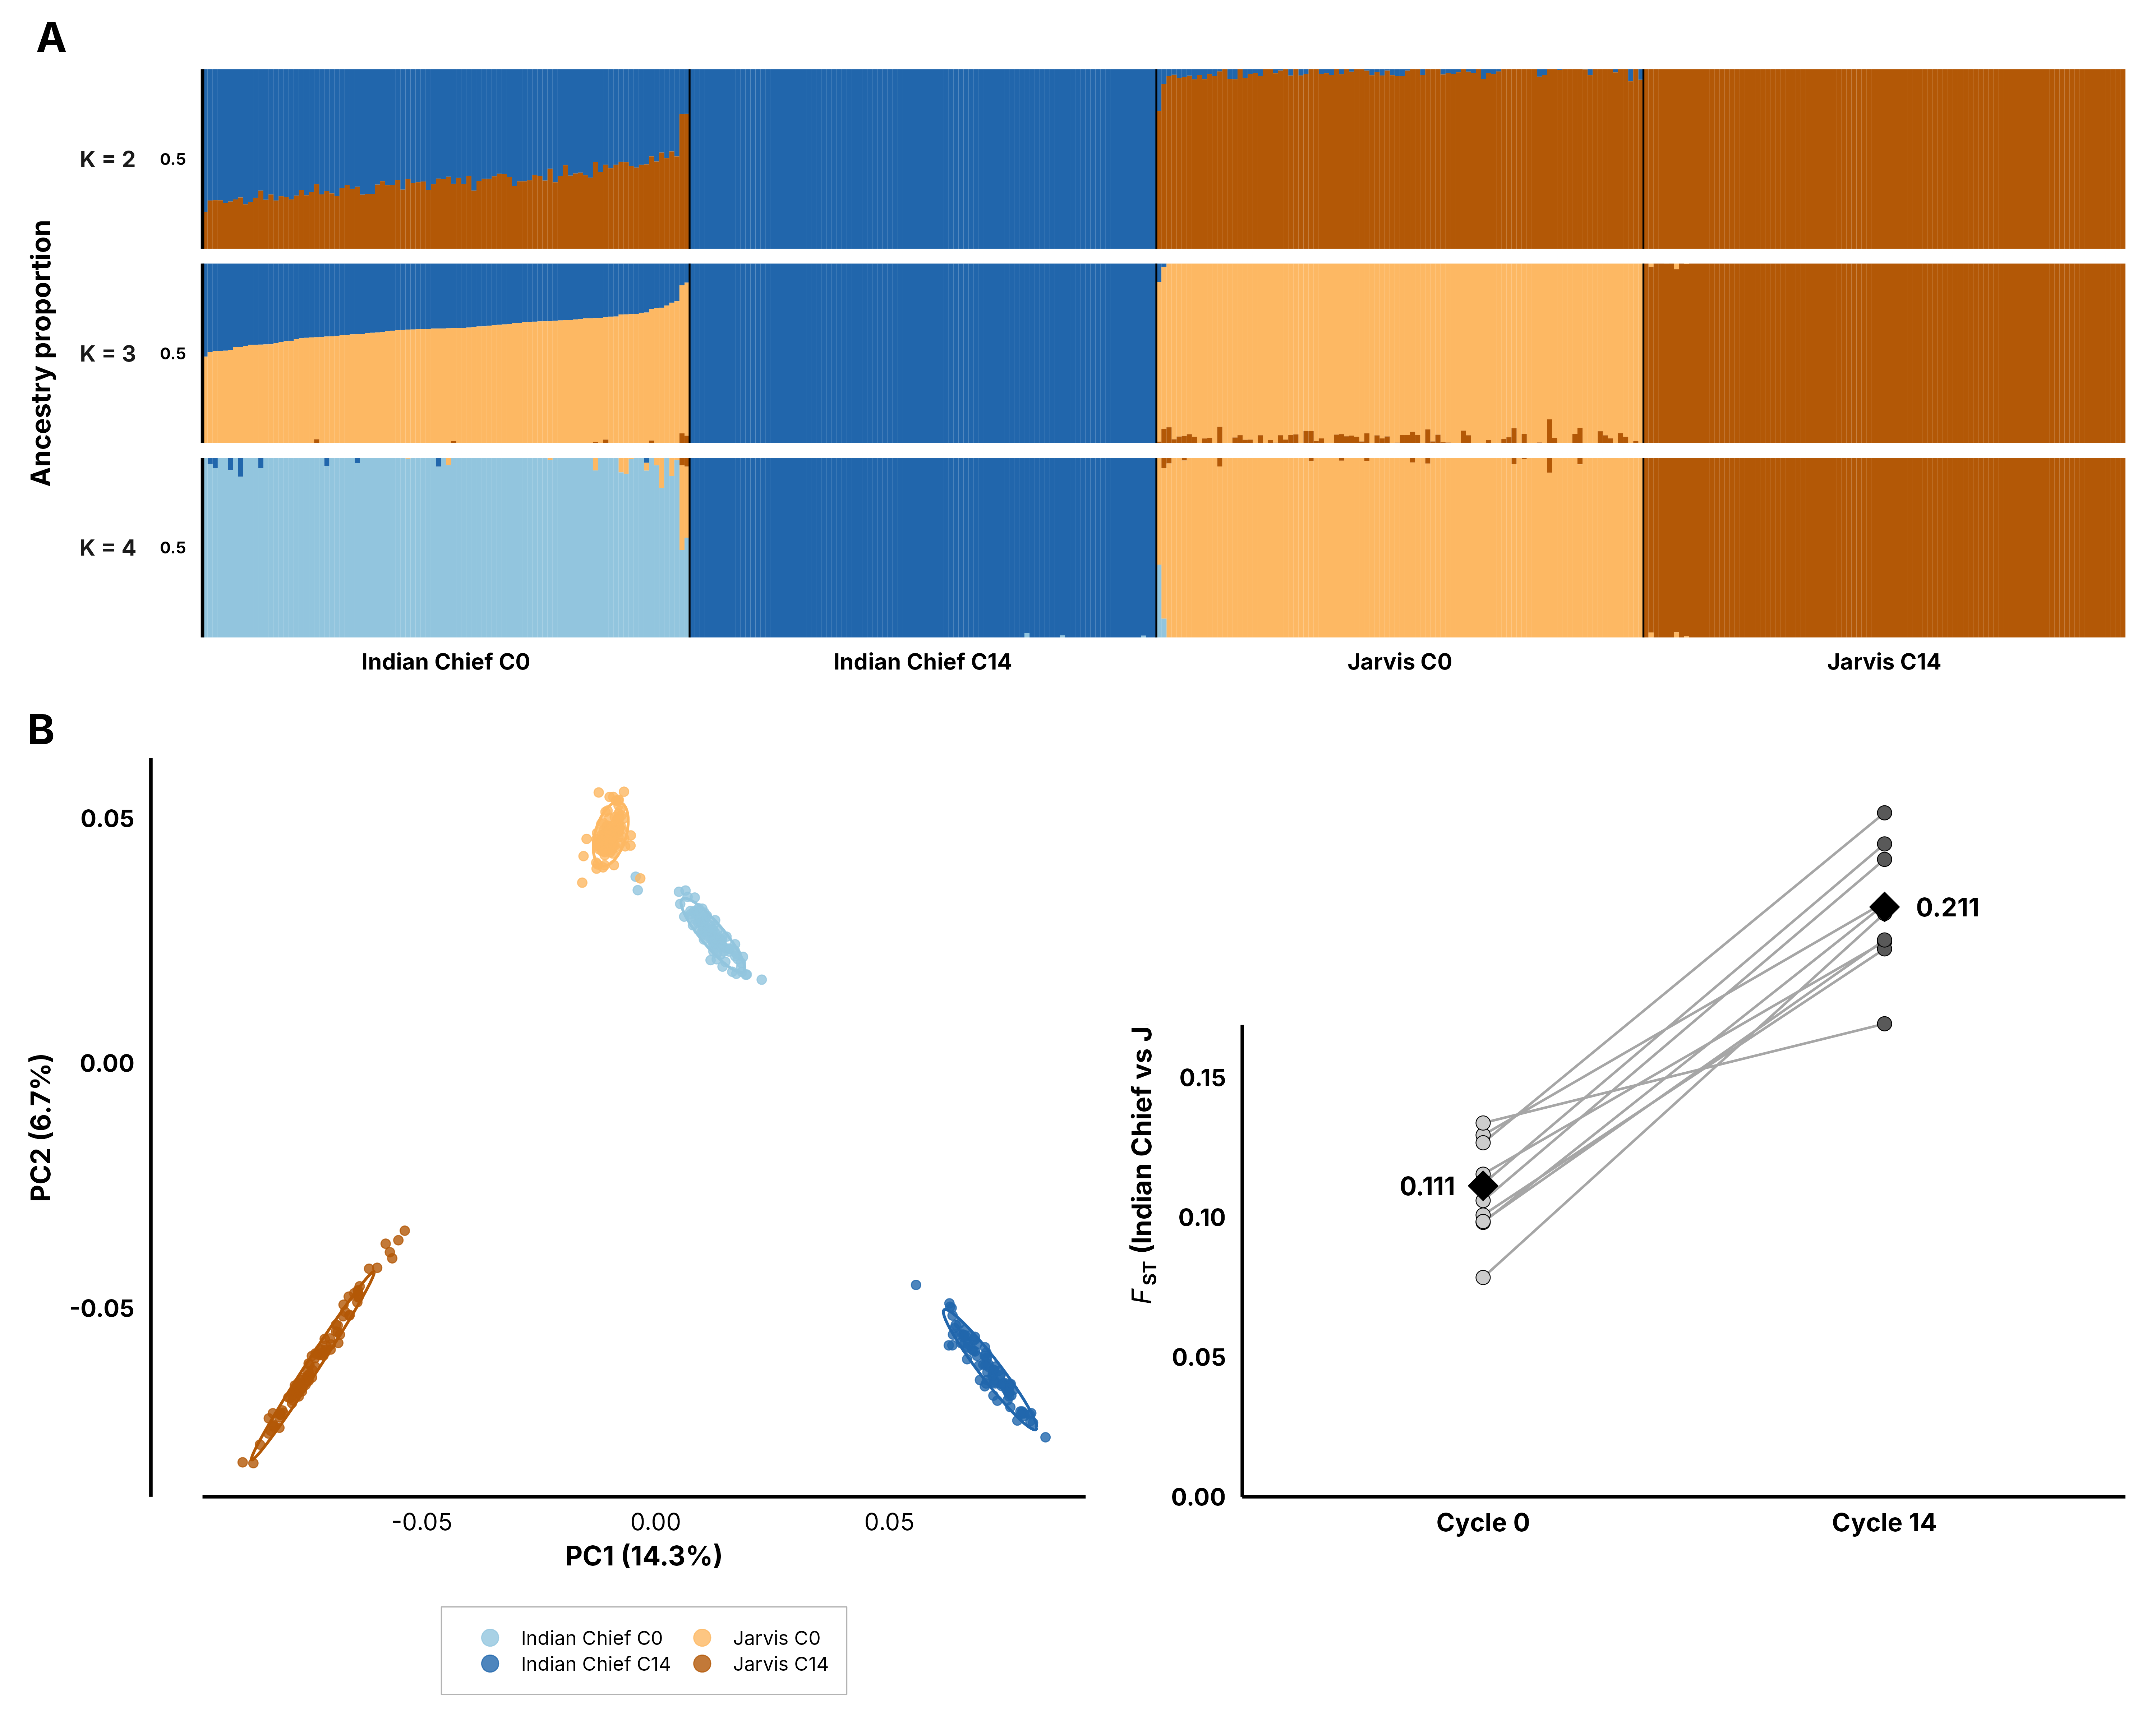
\includegraphics[width=\textwidth]{final/main_figs/Fig4_IC_J_structure.png}
    \caption{\textbf{Indian Chief and Jarvis divergence during 14 cycles of reciprocal recurrent selection.} All panels use genotype likelihoods. \textbf{(A)} Unsupervised ancestry proportions for $K = 2$--4 (thinned to one per 10~kb); each bar is one individual, and each cluster is colored by the group with the highest mean membership. $K = 4$ is the largest $K$ at which independent runs converged. \textbf{(B)} Principal component analysis of the genotype-likelihood covariance matrix; ellipses enclose 90\% of each group. Individuals with lower depth carry less information and lie closer to the centre of their group. \textbf{(C)} $F_{ST}$ between Indian Chief and Jarvis at Cycle 0 and Cycle 14, estimated from the joint site-frequency spectrum of each pair; grey lines connect the same chromosome and black diamonds give the genome-wide value.}
    \label{fig:ic_j_structure}
\end{figure*}

\subsection{$F_{ST}$ scans identify population-specific candidate regions in Indian Chief and Jarvis}

Before scanning for regions of high differentiation between cycles, we asked how much of the allele frequency change could be explained by genetic drift. In the reciprocal recurrent selection program, each cycle was formed by intermating the self-pollinated progenies of the 20 best plants per population \citep{MollStuber1971}, which implies an effective population size ($N_e$) of at most 20 per cycle. Genome-wide mean $F_{ST}$ between Cycle 0 and Cycle 14 was 0.095 in Indian Chief and 0.114 in Jarvis (Fig.~\ref{fig:ic_j_fst}), values reproduced by neutral Wright--Fisher simulations at $N_e \approx 30$ and $N_e \approx 26$ per cycle, respectively (Supplementary Fig.~\ref{fig:supp_ne_drift}). Although slightly above the design-based expectation, these estimates indicate that most genome-wide change between cycles is consistent with drift in small populations. A similar conclusion was reached for the Iowa Stiff Stalk Synthetic (BSSS) and Iowa Corn Borer Synthetic No. 1 (BSCB1), two maize populations under reciprocal recurrent selection for hybrid yield, where linked drift simulations from founder haplotypes explained most of the loss of diversity, and few regions deviated from drift or were shared between populations \citep{Gerke2015DriftRRS}. At this $N_e$, drift moves long linked regions together, so individual outlier regions cannot be formally distinguished from drift. We therefore treat the scans below as exploratory.

We scanned each population for the regions with the largest allele-frequency change between Cycle 0 and Cycle 14 using $F_{ST}$ summarized in windows (2,162 windows in Indian Chief and 2,151 in Jarvis; median length 500 kb). We retained the top 5\% of windows ($F_{ST} \ge 0.157$ in Indian Chief and $\ge 0.178$ in Jarvis; 109 and 108 windows), which contained 2,001 and 1,179 genes, respectively (Fig.~\ref{fig:ic_j_fst}; Supplementary Tables~S18--S21). Candidate regions were largely population-specific. Only five regions (2.5 Mb; 73 genes) were in the top 5\% in both populations, no more than expected by chance ($P = 0.80$; Fig.~\ref{fig:ic_j_fst}), indicating that the two populations show no evidence of shared targets of differentiation. Likewise, 192 of the 2,152 Goodman--Buckler amino acid GWAS loci (8.9\%) fell in a top-5\% window of either population, the same proportion as the genome covered by these windows (8.9\%; $P = 0.52$). Thus, the $F_{ST}$ scans and the amino acid GWAS do not converge on the same genomic regions beyond chance.

Each candidate set contains more than 1,000 genes, so genes from almost any metabolic pathway are expected to be present by chance. We therefore focused on genes in the pathways highlighted by the amino acid and soil N GWAS (Asp-family and Glu/Gln metabolism, amino acid and N transport, and protein turnover) and described them as candidates of interest rather than as evidence of selection. Pathway reoccurence across analyses more than expected is tested in the next section. In Indian Chief, candidate regions included genes of the Asp-family amino acid metabolism, \textit{Zm00001eb214360} (aspartate-semialdehyde dehydrogenase) and \textit{Zm00001eb294790} (threonine synthase), and genes of Glu/Gln interconversion, including two glutamate dehydrogenases (\textit{Zm00001eb060520}, \textit{Zm00001eb162300}), a glutamine synthetase domain-containing protein (\textit{Zm00001eb162900}), and a glutamine amidotransferase domain-containing protein (\textit{Zm00001eb217220}), which also contains a significant SNP for proline in the Goodman--Buckler GWAS (Table~\ref{tab:amino_gwas_focus}). Candidate regions also contained genes involved in N transport and protein turnover, including the senescence-specific cysteine protease \textit{SAG39} (\textit{Zm00001eb214780}) and an ammonium transporter (\textit{Zm00001eb214890}), which lie in the same window on chromosome 5; an NRT1/PTR-family transporter (\textit{Zm00001eb287950}) and the autophagy-related gene \textit{ATG18g} (\textit{Zm00001eb287690}), which share a window on chromosome 6, as well as two further autophagy-related genes (\textit{Zm00001eb352300} and \textit{Zm00001eb372060}). These annotations are compatible with the Indian Chief FAA phenotype, in which total FAA and the Pro fraction increased while the Asp and Glu fractions decreased from Cycle 0 to Cycle 14, but they do not establish that these genes underlie it.

In Jarvis, candidate regions included two genes of Asp metabolism, including \textit{Zm00001eb094670}, annotated as aspartate kinase, and an aspartate aminotransferase (\textit{Zm00001eb152450}, GOT1/THP3). These genes are of interest because the Asp fraction was the only FAA trait that changed in Jarvis, increasing nominally from Cycle 0 to Cycle 14. Jarvis candidate regions also contained two amino acid transporter genes (\textit{Zm00001eb132750}, an amino acid transporter transmembrane domain-containing protein, and \textit{Zm00001eb159580}, a putative GABA transporter), NPL4-like protein 1 (\textit{Zm00001eb146560}), which acts in ubiquitin-dependent protein degradation, and two glutaredoxins (\textit{Zm00001eb131830} and \textit{Zm00001eb131840}). As in Indian Chief, these candidates point to amino acid metabolism, transport, and protein turnover as processes worth testing, but they require functional validation.

%===================== FIGURE 5 =====================
\begin{figure*}[ht!]
    \centering
    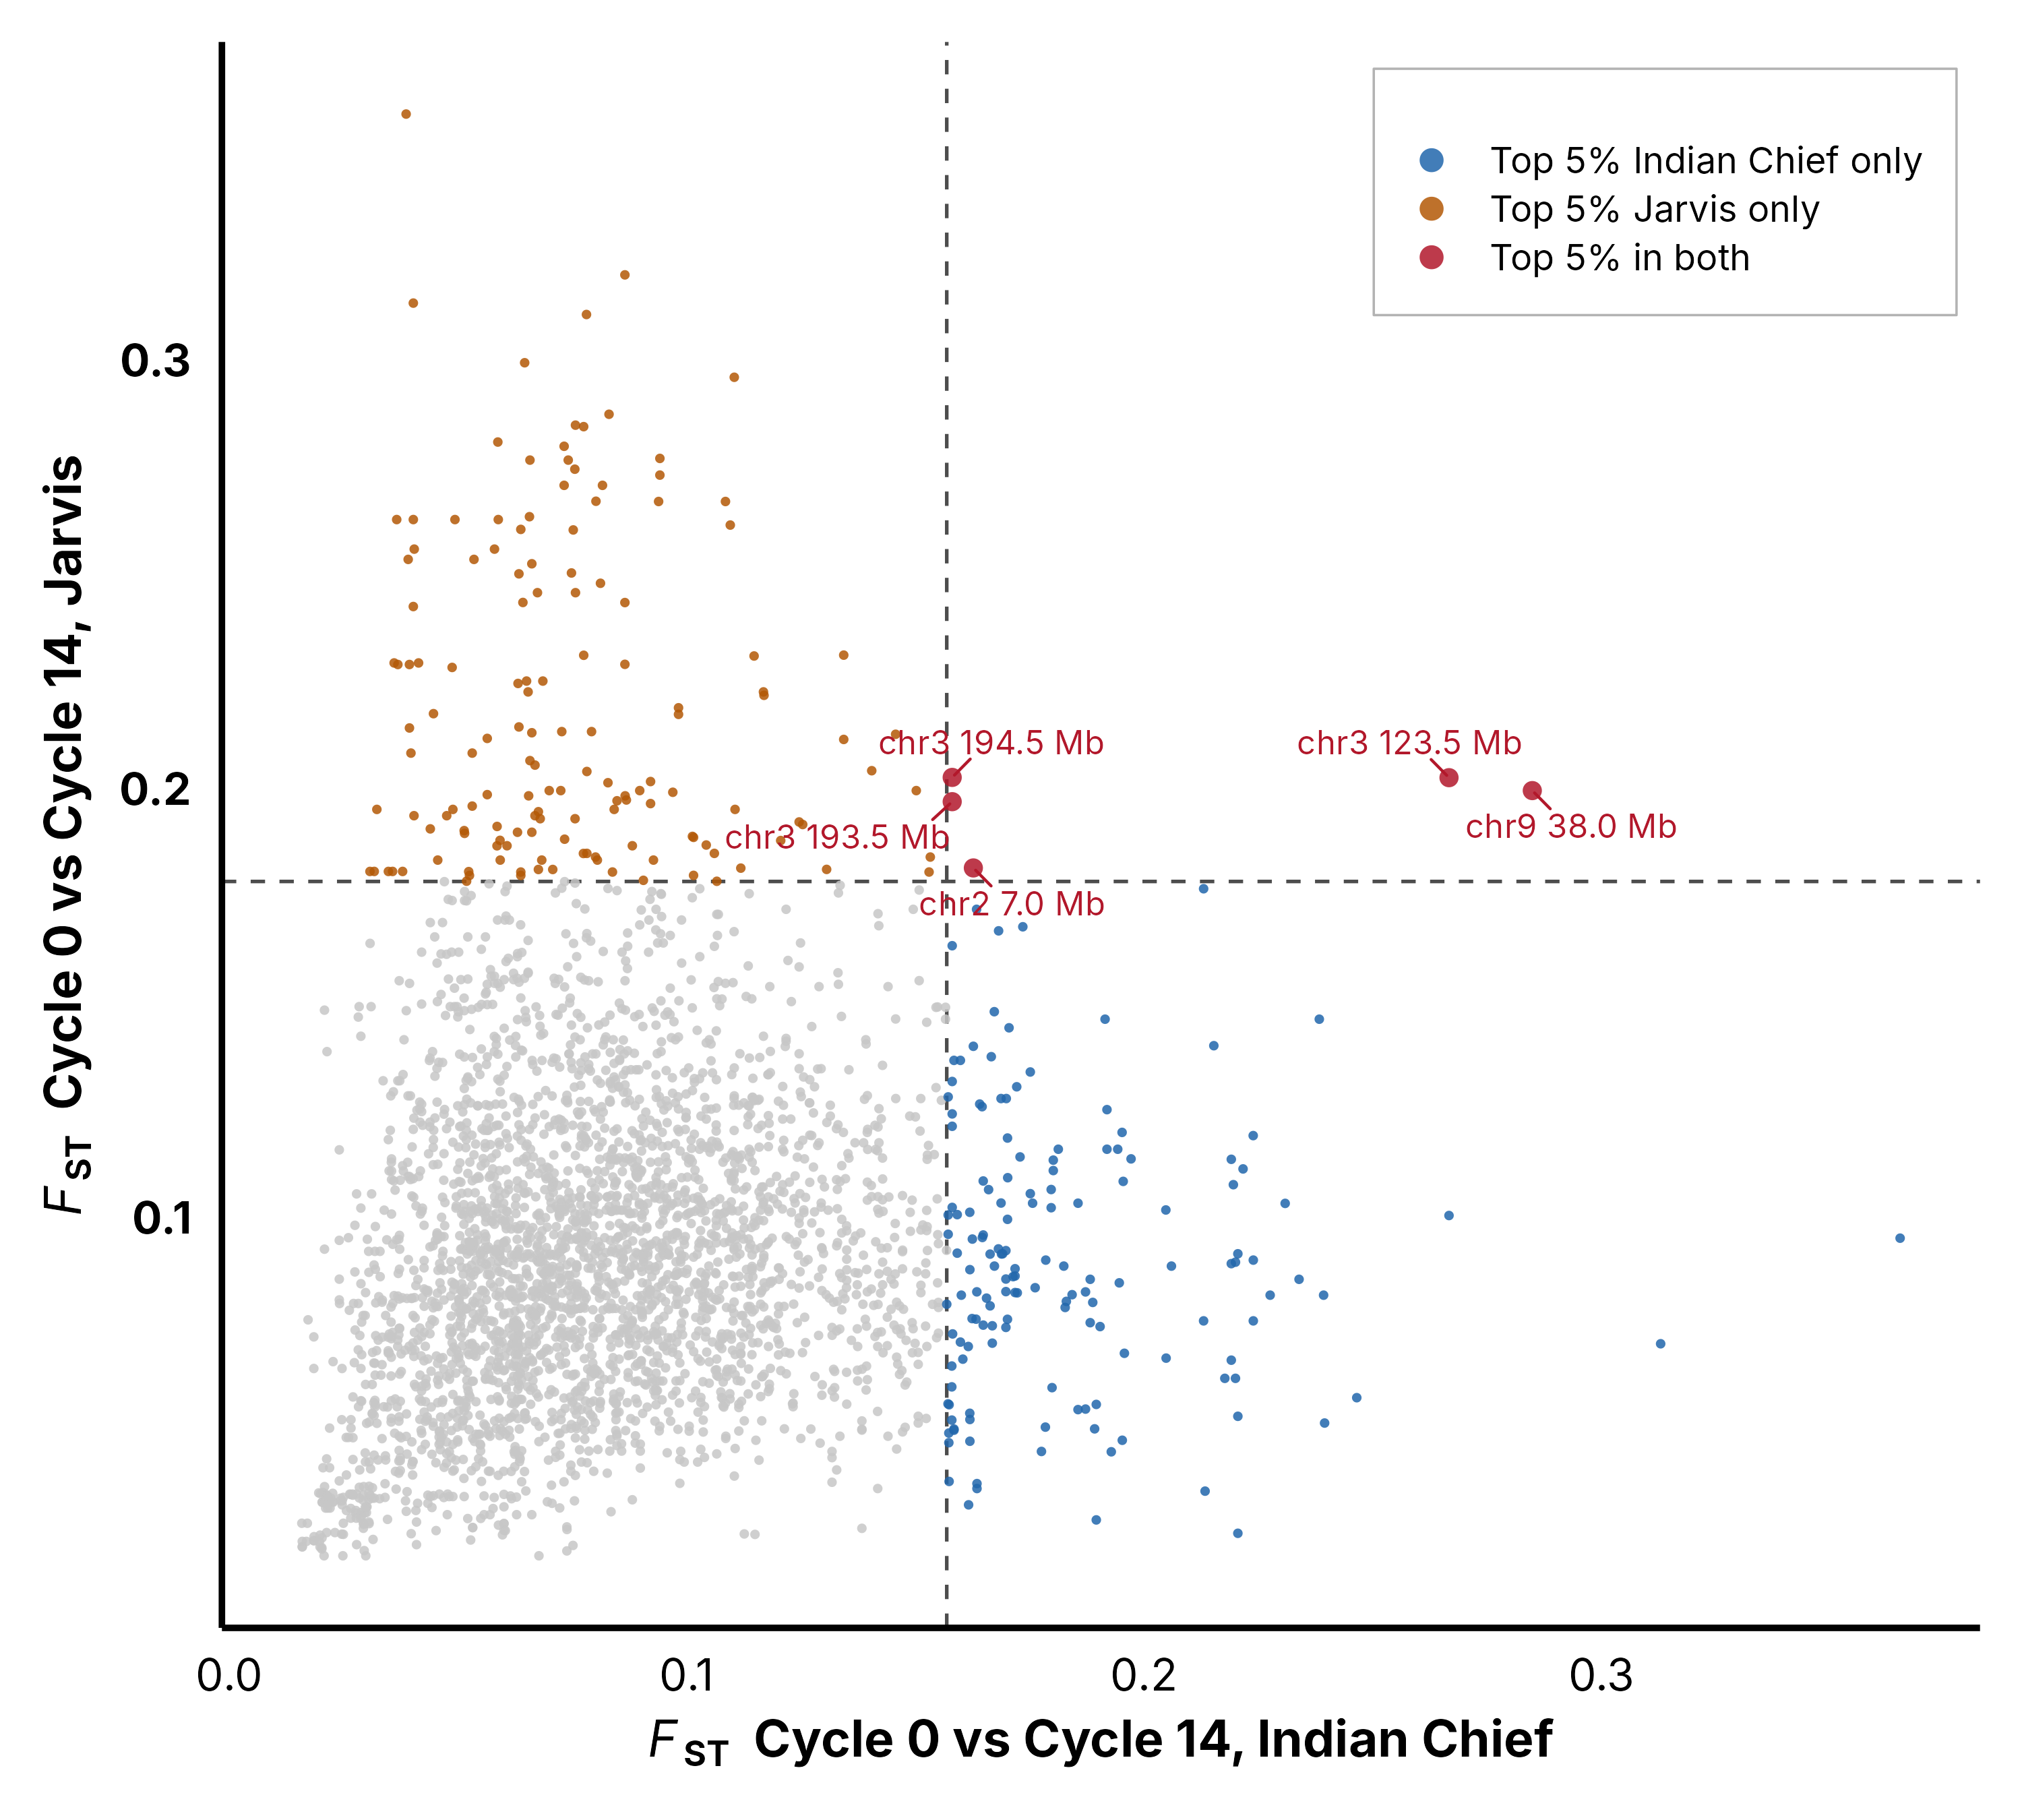
\includegraphics[width=0.75\textwidth]{final/main_figs/Fig5_IC_J_Fst_scan.png}
    \caption{\textbf{Candidate regions of differentiation between Cycle 0 and Cycle 14} $F_{ST}$ between Cycle 0 and Cycle 14 in Indian Chief ($x$-axis) and Jarvis ($y$-axis), estimated from genotype likelihoods and summarized in spline-defined windows. Each point is a genomic segment bounded by the window boundaries of either population, and carries the $F_{ST}$ of the Indian Chief and Jarvis windows that contain it. Dashed lines mark the top 5\% of windows in each population ($F_{ST} \geq 0.157$ in Indian Chief and $\geq 0.178$ in Jarvis). Blue and orange, top 5\% in one population only; red, top 5\% in both, labeled with chromosome and position.}
    \label{fig:ic_j_fst}
\end{figure*}

\subsection{The aspartate-to-homoserine pathway recurs across the three populations}

To test whether the three populations implicate the same metabolic pathways, we asked whether any CornCyc pathway \citep{Hawkins2021PMN} contained candidate genes from more than one of the four analyses (amino acid GWAS, soil N GWAS, and the Indian Chief and Jarvis $F_{ST}$ scans) more often than expected by chance. We represented each candidate set by its genomic intervals and generated a null distribution by randomly shifting the intervals along each chromosome, which preserves their number, size, and clustering. Because this test asks whether one pathway stands out from all others, larger candidate sets add background genes that hit many pathways by chance. Therefore, we used stricter sets than in the gene level analyses. The bonferroni significant SNPs for both GWAS and the top 3\% of $F_{ST}$ windows. Among 468 pathways, L-homoserine biosynthesis had candidates from all four analyses, had the lowest permutation-based empirical $P$ ($P = 0.00034$), and was the only pathway that remained significant after correction across all pathways (corrected $P = 0.021$; Fig.~\ref{fig:pathway_recurrence}). Each analysis implicated a different enzyme, homoserine dehydrogenase (\textit{Zm00001eb405410}) in the amino acid GWAS (Asn relative to the Asp-family amino acids, \textit{N.IMNTDK}), an aspartate kinase isozyme (\textit{Zm00001eb220040}) in the soil N GWAS, aspartate-semialdehyde dehydrogenase (\textit{Zm00001eb214360}) in Indian Chief, and aspartate kinase (\textit{Zm00001eb094670}) in Jarvis. L-lysine biosynthesis VI also had candidates from all four analyses ($P = 0.0030$), largely because it shares the aspartate kinase and aspartate-semialdehyde dehydrogenase steps. The other pathways with $P < 0.05$ were small terpenoid and vitamin E pathways with candidates from two or three analyses, and none remained significant after correction.

We reran the test across 12 combinations of GWAS thresholds (FDR 5\%, 3\%, 1\%, and Bonferroni) and $F_{ST}$ window thresholds (top 5\%, 3\%, 1\%) (Supplementary Fig.~\ref{suppfig:pathway_thresholds}). The same four genes were recovered at all GWAS thresholds when using the top 5\% or 3\% of $F_{ST}$ windows, and in all eight such combinations, L-homoserine biosynthesis ranked first or second among 468 pathways. Across all 12 combinations, it ranked first five times and second three times. The lower ranks occurred only with the top 1\% windows (Supplementary Fig.~\ref{suppfig:pathway_thresholds}B). Using larger candidate sets (FDR 5\% and top 5\% windows), more pathways were hit by chance, and the pathway was not significant after correction (corrected $P=0.68$). Thus, L-homoserine biosynthesis ranked consistently across thresholds, while corrected significance depended on candidate-set size. Although candidate regions from the four analyses overlap no more than expected by chance, each implicates a different step in aspartate-to-homoserine conversion.

\begin{figure*}[ht!]
  \centering
  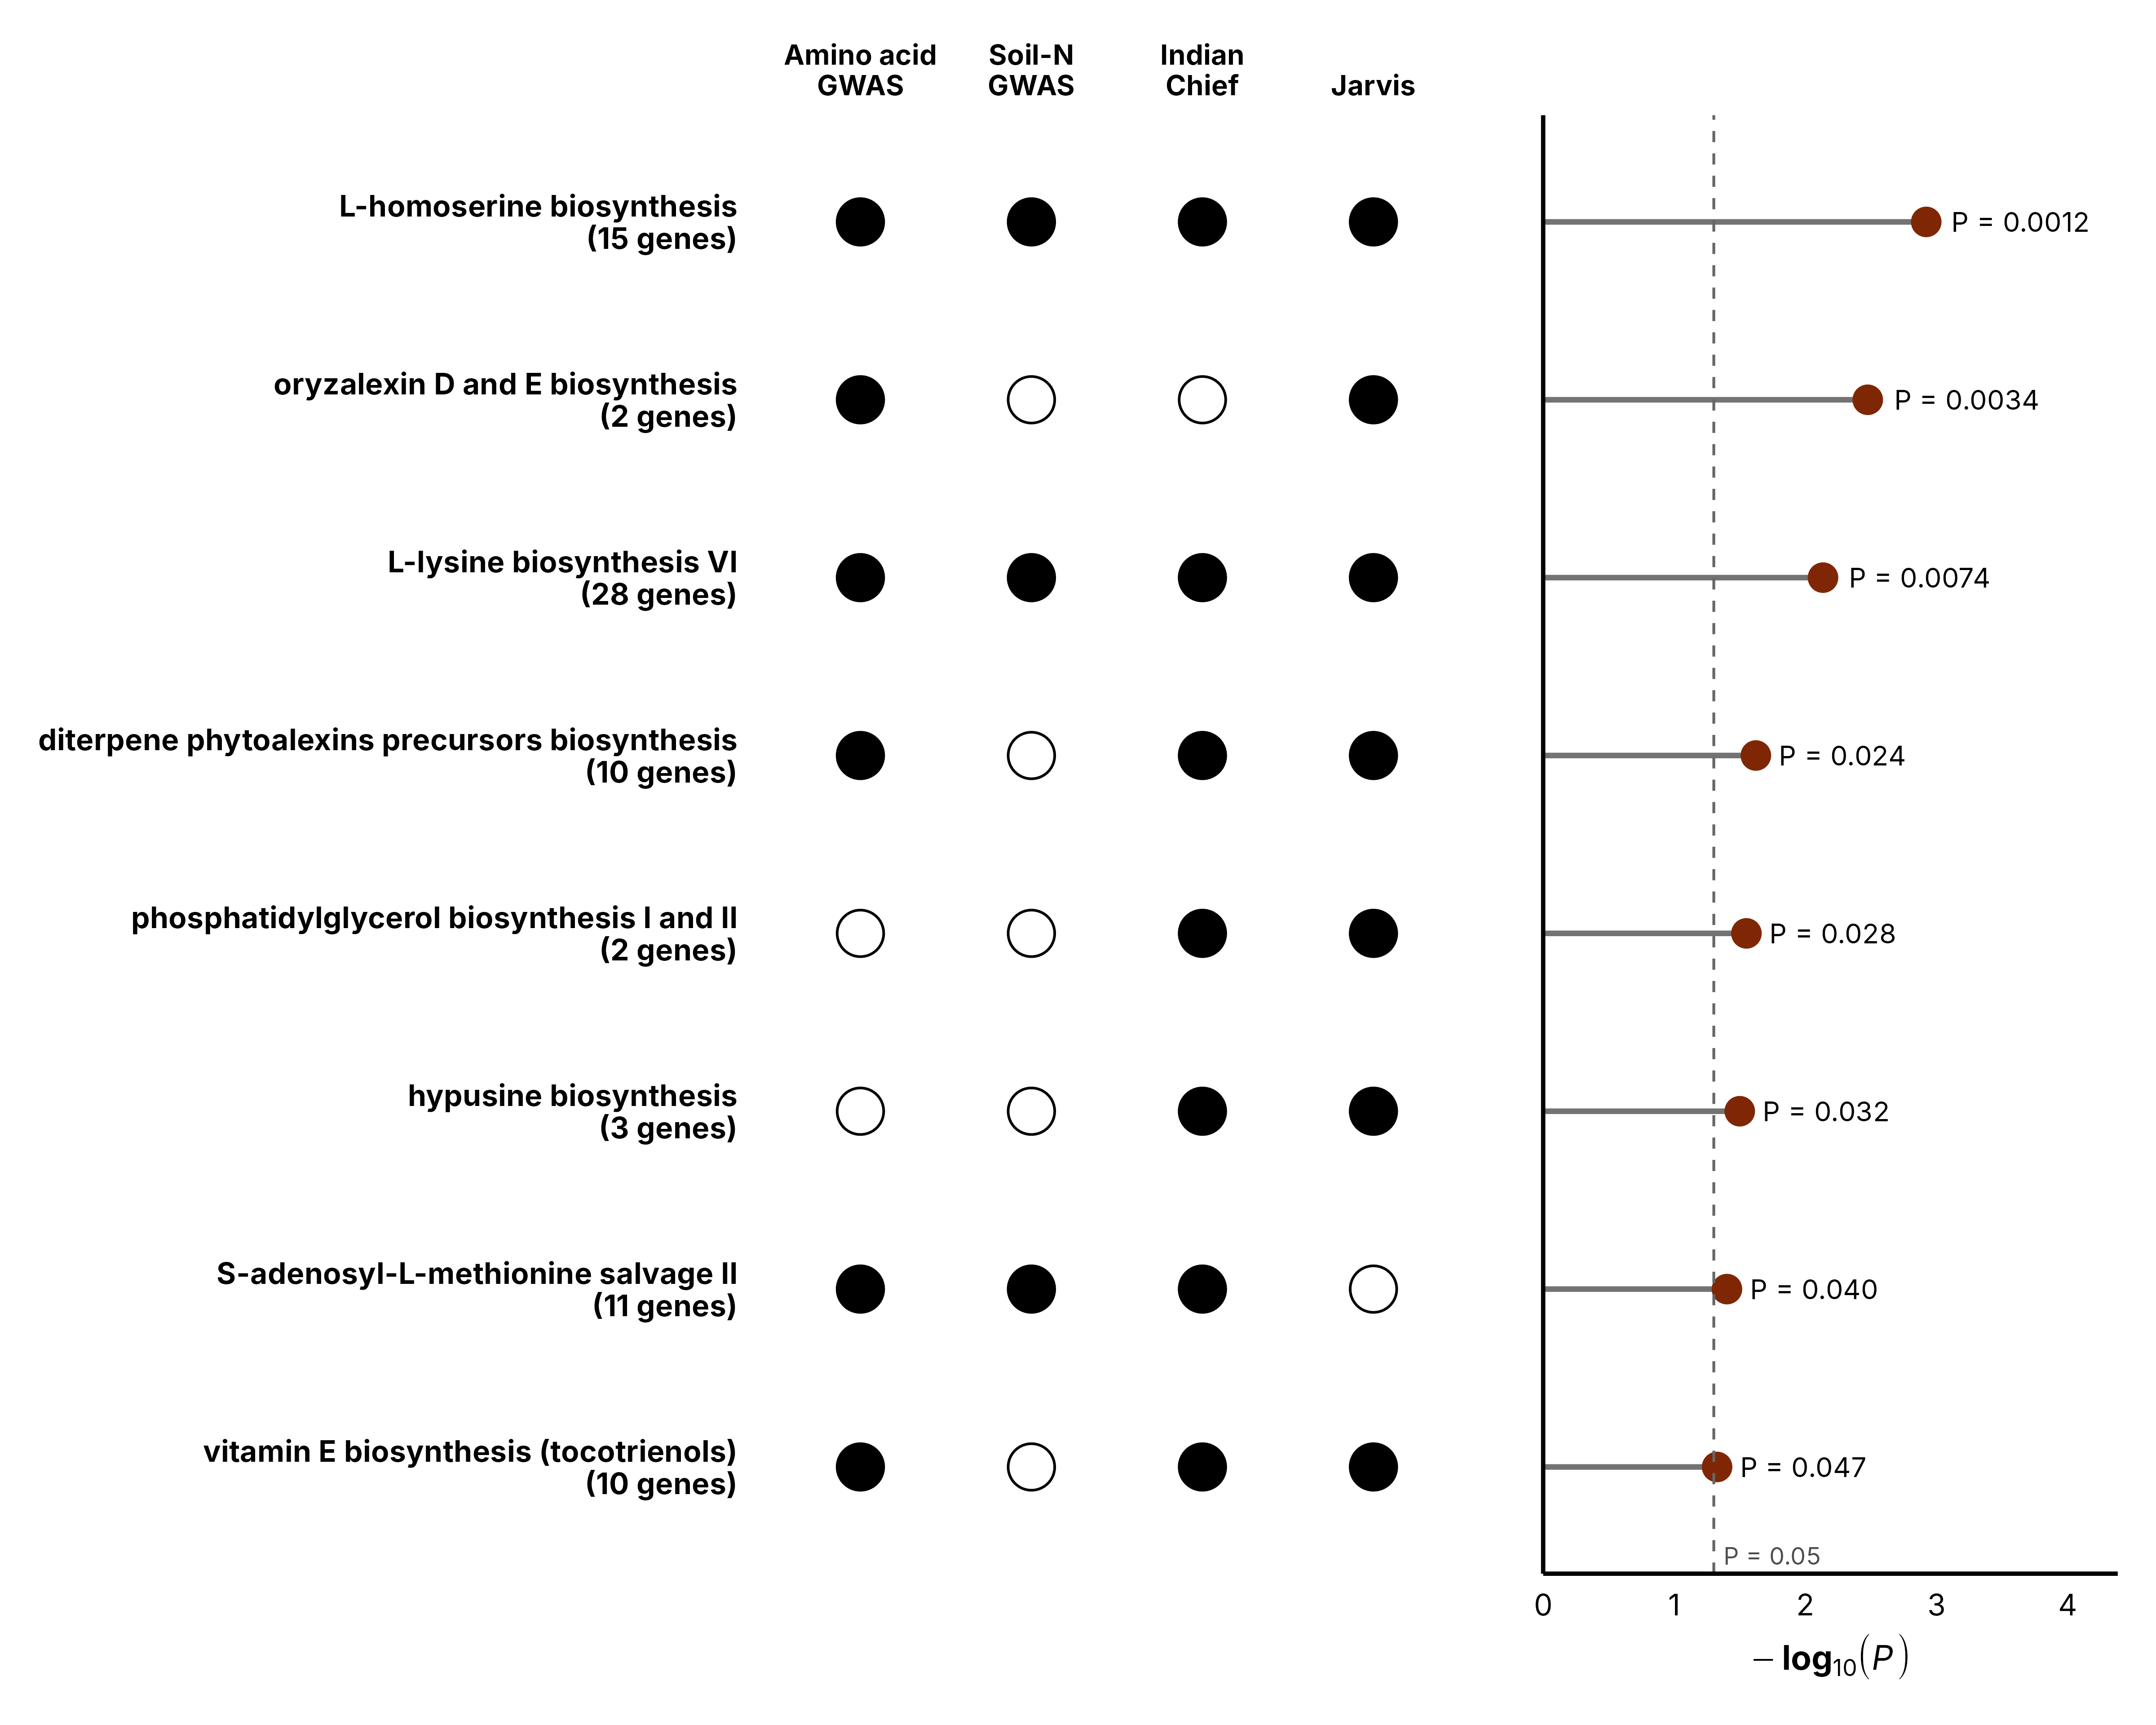
\includegraphics[width=\textwidth]{final/main_figs/Fig_pathway_recurrence.png}
    \caption{\textbf{The L-homoserine biosynthesis pathway recurs across all four analyses.} All CornCyc pathways with uncorrected permutation $P < 0.05$ for recurrence across the amino acid GWAS, soil-N GWAS and the Indian Chief and Jarvis $F_{ST}$ scans, using Bonferroni-significant GWAS SNPs and the top 3\% of $F_{ST}$ windows. Left, filled circles mark analyses with at least one candidate gene in the pathway; numbers in brackets give the number of maize genes in the pathway. Right, pathway-specific permutation-based empirical $P$ for the observed number of analyses hitting the pathway; dashed line, $P = 0.05$. The corrected $P$ (minimum-$P$ correction across all 468 pathways) is shown for the only pathway that remained significant.}
  \label{fig:pathway_recurrence}
\end{figure*}

\section{Discussion}

We tested whether natural variation in grain amino acids, genetic variation linked to soil N, and yield selection implicate the same N-metabolism functions in maize. In the Goodman–Buckler panel, the free amino acid pool was small, dominated by Asn and Pro, highly variable, and heritable. GWAS highlighted candidates for amino acid metabolism, transport, and protein turnover. In landraces, soil N at the collection site associated with SNPs near an aspartate kinase isozyme and an $\omega$-amidase, surviving controls for geographic and climatic confounding. After 14 cycles of reciprocal recurrent selection for yield, Indian Chief and Jarvis differed in how they allocated N, with Jarvis increasing grain N mainly through post-anthesis N uptake and Indian Chief retaining more N in the stover \citep{Moll1994}. In our samples, Indian Chief also accumulated more free amino acids, mostly Pro, and the two populations diverged further genetically. Although most candidates were analysis-specific, each analysis implicated a different enzyme in the aspartate-to-homoserine pathway, the only pathway that remained significant after correction. Next, we analyze multi-trait loci, the aspartate-to-homoserine pathway, and the aspartate–glutamate junction, along with candidate genes involved in transport and protein turnover. These annotation-based candidates require functional validation.

\subsection{Loci shared by many amino acid traits point to protein turnover and membrane protein biogenesis rather than specific biosynthetic steps}

Few GWAS loci were shared across many amino acid phenotypes. Phenotype counts also overstate independent signals because composites and ratios reuse amino acids. The most interpretable case is the chromosome 4 locus at 174.57 Mb, associated with eight phenotypes (including Ala, Val, Lys, Phe, and Thr) spanning four biosynthetic families, and adjacent to \textit{Zm00001eb190800}, encoding a peptidase A1 (pepsin-like aspartic protease) (Fig.~\ref{fig:amino_locus_manhattan}). Aspartic proteases are known to drive bulk protein turnover. In senescing tobacco, chloroplast CND41 degrades Rubisco, and reduced CND41 increases Rubisco retention under N limitation \citep{Kato2004CND41}. Rubisco breakdown is a major source of amino acids released during senescence \citep{Feller2008Rubiscolytics}, although A1 proteases also act in development and stress responses \citep{Soares2019AtypicalAP}. A single locus affecting amino acids from four biosynthetic families is more easily explained by a change in protein degradation than by a change in one biosynthetic enzyme, which makes \textit{Zm00001eb190800} a plausible candidate for functional testing.

The chromosome 9 locus implicates the endomembrane system. A $\sim$13 kb region associated with nine phenotypes (including total free amino acids) spans \textit{Zm00001eb394360} and \textit{Zm00001eb394380}. \textit{Zm00001eb394360} encodes ER membrane protein complex subunit 4, which inserts transmembrane proteins into the ER \citep{Guna2018EMC}, and \textit{Zm00001eb394380} encodes rhomboid-like protein 19, an intramembrane serine protease annotated for Golgi-to-ER retrograde transport. Although the functions of most plant rhomboid-like proteins remain unknown \citep{Lavell2021RBL10}, both genes act in the ER--Golgi system that processes transporters and secreted proteins involved in amino acid and N movement \citep{Brandizzi2018ERGolgi}, so either could affect the overall free amino acid pool. Because the associations do not clearly separate these genes from nearby genes (including a DUF2404 membrane protein at the chromosome 4 locus), both loci should be treated as positional candidates, and kernel expression and mutant analyses are the most direct tests. Candidate annotations, trait associations, and model-specific GWAS results are available at \url{https://j83gk2-nirwan-tandukar.shinyapps.io/amino_gwas_app/}.

\subsection{The aspartate-to-homoserine pathway links soil-N adaptation, recurrent selection, and grain amino acid variation}

Asparagine was the most abundant free amino acid in the Goodman--Buckler panel and, because of its high N-to-C ratio, is a major N transport and storage form in plants \citep{Lea2007Asparagine}. It is synthesized from Asp by asparagine synthetase using the amide N of Gln, and catabolism returns carbon to Asp or oxaloacetate \citep{Lea2007Asparagine}. Asp is thus both the precursor of Asn and the entry point to the Asp-family pathway that produces Lys, Thr, Met, and Ile \citep{Han2021Aspartate, Wang2018AspSeeds, Viola2001AspartatePathway}. Pathway flux is regulated mainly by feedback inhibition of aspartate kinase by Lys and Thr, and of dihydrodipicolinate synthase by Lys \citep{Azevedo2006AspPathway, Jander2009AspArabidopsis}. This pathway was implicated by all four analyses. L-homoserine biosynthesis had a candidate gene in every analysis, had the lowest permutation-based empirical $P$ of the 468 CornCyc pathways, and was the only pathway that remained significant after correction (Fig.~\ref{fig:pathway_recurrence}).

Across analyses, implicated genes spanned the Asp to homoserine pathway. Jarvis regions included aspartate kinase (\textit{Zm00001eb094670}), the first committed step \citep{Viola2001AspartatePathway}, and \textit{ask2} expression is linked to Met accumulation in developing kernels \citep{Duo2026Ask2}. The only soil N SNP significant in all three GWAS models, which also passed both tests for confounding with geography and climate, was near another aspartate kinase (\textit{Zm00001eb220040}). Indian Chief regions included aspartate-semialdehyde dehydrogenase (\textit{Zm00001eb214360}), and the amino acid GWAS implicated homoserine dehydrogenase (\textit{Zm00001eb405410}), the first committed step to Thr and Met. Further downstream, Indian Chief regions included threonine synthase (\textit{Zm00001eb294790}) and methionine synthase (\textit{Zm00001eb052750}), the latter also near a soil-N SNP. The amino acid GWAS also identified genes in the Lys branch, dihydrodipicolinate synthase (\textit{Zm00001eb389290}), dihydrodipicolinate reductase (\textit{Zm00001eb176170}), and diaminopimelate decarboxylase (\textit{Zm00001eb406820}), and in the Asn branch, two asparagine synthetase domain genes (\textit{Zm00001eb036060}, \textit{Zm00001eb036070}) and the amino acid transporter AVT6C (\textit{Zm00001eb368680}), suggesting that transport or storage, not only synthesis, may shape the Asn pool.

Together, three populations with different germplasm and study designs point to the same short pathway, with each analysis implicating a different enzyme. This pattern did not depend on a single threshold. Candidate thresholds are conventions, and across GWAS and $F_{ST}$ thresholds, the same four genes were recovered, with L-homoserine biosynthesis ranked first or second among 468 pathways. It became significant after correction when stricter sets reduced the number of background genes (Supplementary Fig.~\ref{suppfig:pathway_thresholds}), so its consistent ranking is more informative than any single $P$ value. Drift could still contribute to the $F_{ST}$ candidate regions given $N_e \approx 25$--30 (Supplementary Fig.~\ref{fig:supp_ne_drift}), and soil N candidates may reflect local adaptation even though they passed tests for geography and climate. For the two soil-N candidates, the minor alleles came from many independent collection sites and were more frequent at N-rich sites, most clearly for $\omega$-amidase within Mexico (Supplementary Fig.~\ref{suppfig:soilN_focal_geography}), so neither signal rests on a single site, although shared ancestry may contribute. 

Therefore, these genes are strong candidates for direct tests, such as comparing Asp-family amino acids among lines with alternative alleles at \textit{Zm00001eb405410}, \textit{Zm00001eb220040}, \textit{Zm00001eb214360}, and \textit{Zm00001eb094670}. Aspartate is a branch point in plant N metabolism. It is the precursor of Asn, a major transport and storage form of N \citep{Lea2007Asparagine}. It also exchanges amino groups with Glu via transamination, and it is synthesized from the TCA cycle intermediate oxaloacetate, linking amino-acid N to carbon metabolism \citep{Han2021Aspartate}. Variation at the entry to the Asp-family pathway could shift how Asp-derived N is allocated among Asn, Asp-family amino acids, and the Glu/Gln pool, consistent with the association of an aspartate kinase allele with soil N in landraces. Links from Asp to Glu/Gln and the $\omega$-amidase pathway are discussed next.

\subsection{Candidate genes at the aspartate--glutamate junction link amino acid N with C--N recycling}

Glutamate exchanges amino groups with the TCA-cycle intermediate 2-oxoglutarate, which provides the carbon skeleton for ammonium assimilation through the GS/GOGAT cycle and glutamate dehydrogenase, and whose level signals C and N status in many organisms \citep{Huergo2015TwoOG}. Together, Asp, Asn, Glu, and Gln make up most of the free amino acid pool and are major N transport forms in plants \citep{McAllister2016AAT}. Because no Glu/Gln pathway recurred across analyses, we discuss these junction candidates individually.

Each analysis implicated different genes at the junction. On the Asp side, Jarvis regions contained the aspartate aminotransferase \textit{Zm00001eb152450} (GOT1), which interconverts Asp and 2-oxoglutarate with oxaloacetate and Glu \citep{Han2021Aspartate, Zhou2009AspAT}. This gene was recently identified as \textit{THP3}, whose teosinte alleles improve N assimilation and seed protein in maize \citep{Huang2026THP3}. In contrast, overexpressing a cytosolic aspartate aminotransferase from alfalfa in \textit{Brassica napus} did not increase N use efficiency \citep{McAllister2016AAT}, suggesting that the effects of this enzyme depend on the isoform and the tissue in which it is expressed. The soil-N GWAS identified an $\omega$-amidase (\textit{Zm00001eb005710}) that completes Asn/Gln transaminase routes by returning carbon to oxaloacetate and 2-oxoglutarate while releasing ammonia \citep{Zhang2014OmegaAmidase}.

On the Glu side, the clearest case is Indian Chief, the only population whose free amino acid profile changed (Fig.~\ref{fig:ic_j_faa}). Most of the Cycle 14 increase in total free amino acids was Pro, so the lower Asp and Glu fractions largely reflect Pro accumulation. Indian Chief regions included two glutamate dehydrogenases (\textit{Zm00001eb060520}, \textit{Zm00001eb162300}), a glutamine synthetase (\textit{Zm00001eb162900}), and a class I glutamine amidotransferase (\textit{Zm00001eb217220}) that was also a candidate for free Pro in the amino acid GWAS, but no genes for Pro synthesis. GDH mutants show altered amino acid profiles under carbon limitation \citep{Miyashita2008GDH, Dellero2020AminoNUE}, and cereal GS supplies Gln to developing grain \citep{Wei2021WheatGS, Fujita2022RiceGS13}. Because Pro is synthesized from Glu \citep{Lehmann2010ProMetab, Alvarez2022ProHub}, increased flux from Glu to Pro, rather than increased primary N assimilation, is a plausible explanation, although we did not measure flux or enzyme activity. Glutamine amidotransferases function broadly, so \textit{Zm00001eb217220} cannot be assigned to the Glu/Gln cycle without functional evidence, although rice \textit{FLOURY ENDOSPERM19} affects grain filling and C--N metabolism \citep{Lou2021FLO19}. Because most grain N is protein-bound, these shifts changed the soluble pool without affecting total grain amino acid N. Jarvis showed no corrected change, consistent with \citet{Moll1994}, in which its grain N gain came mainly from higher grain weight and post-anthesis N uptake. In the amino acid GWAS, GS/GOGAT genes (\textit{Zm00001eb329710}, \textit{Zm00001eb360480}, \textit{Zm00001eb059870}) were associated with ratio traits, including Asn/Glu. Thus, all three populations implicated genes at the junction where Asp and Glu exchange N with TCA-cycle carbon. These genes differ among analyses and lack pathway-level support, but finding the same junction in three independent designs makes it a priority for testing how maize balances amino acid N against carbon supply.

\subsection{Amino acid transport and protein turnover candidates}

Beyond Asp and Glu metabolism, each analysis contained candidates for amino acid transport or protein turnover, and these differed among populations in ways that matched their phenotypes. They are individual candidates rather than recurring pathways, and because $F_{ST}$ windows in small populations can reflect drift \citep{Gerke2015DriftRRS}, we considered Indian Chief and Jarvis candidates only when they matched the amino acid phenotypes.

Protein-turnover candidates were most relevant in Indian Chief, where Cycle 14 grain had higher free amino acids but unchanged protein-bound amino acids. Candidate regions included \textit{Zm00001eb352300}, homologous to Arabidopsis \textit{ATG18a} required for autophagosome formation during nutrient stress and senescence \citep{Xiong2005ATG18a}, and the cysteine protease \textit{SAG39} (\textit{Zm00001eb214780}). Its Arabidopsis homolog \textit{SAG12} localizes to senescence-associated vacuoles \citep{Otegui2005SAV} and supports N allocation to seeds \citep{James2018SAG12}. The same window also contained \textit{Zm00001eb214890}, homologous to the ammonium transporter \textit{AtAMT2} \citep{Neuhaeuser2009AtAMT2}. Increased protease or autophagy activity in Cycle 14 could expand the free amino acid pool, but these activities were not measured.

Jarvis candidate regions instead contained genes involved in amino acid import and N signaling. An LHT-like gene (\textit{Zm00001eb132750}) encodes a plasma membrane amino acid importer. In Arabidopsis, LHT1 imports amino acids into root and leaf cells, reducing losses \citep{Fan2023LHT}. A ProT-like gene (\textit{Zm00001eb159580}) transports Pro, glycine betaine, and GABA between cells \citep{Lehmann2011ProT}. These regions also included a tandem pair of CC-type glutaredoxin genes (\textit{Zm00001eb131830}, \textit{Zm00001eb131840}) in two highly differentiated windows (ranked 2nd and 7th out of 2,151). In a reanalysis of public maize leaf RNA-seq data \citep{Mu2017LN, Guo2022LN, Ma2021LN, TorresRodriguez2021LN, AlonsoNieves2022LN, Wang2025NRT25}, both genes were strongly downregulated under low nitrate (\textit{Zm00001eb131840}; about 80-fold lower), although their expression in developing kernels is unknown (Supplementary Table~S22). In Arabidopsis, CC-type glutaredoxins function in N signaling, including nitrate-induced regulators of root growth and the mobile peptides CEPD1/CEPD2 that increase nitrate uptake under N demand \citep{Patterson2016GRX, Ohkubo2017CEPD}. Both glutaredoxin genes and the LHT-like gene also lie within the chromosome 3 Asp and Pro QTL interval of the B64 $\times$ CML14 population (Supplementary Fig.~\ref{suppfig:qtl_asp_pro}). Because Jarvis increased grain N mainly via post-anthesis N uptake \citep{Moll1994}, amino acid import and N-signaling genes may be more relevant than changes in grain amino acid composition. Jarvis regions also contained NPL4-like protein 1 (\textit{Zm00001eb146560}). Its Arabidopsis homolog partners with UFD1 and CDC48 to target ubiquitinated proteins (including Rubisco large subunit) for proteasomal degradation \citep{Li2022CDC48}.

In the amino acid GWAS, several transporter candidates mapped to specific free amino acids. Three UmamiT genes (WAT1-related exporters) were associated with Gln (\textit{Zm00001eb379220}), Asp (\textit{Zm00001eb207630}), and Lys (\textit{Zm00001eb352400}). Because seed-coat UmamiTs export maternal amino acids to the embryo and mutants reduce supply \citep{Muller2015UmamiT}, these associations suggest that variation in export to the grain can alter individual free amino acids without changing synthesis. The NRT1/PTR family gene \textit{NPF4.6} (\textit{Zm00001eb277160}), whose family transports nitrate, peptides, amino acids, and hormones \citep{Leran2014NPF}, was linked to free Lys. The Gln/Glu ratio mapped to the amino acid permease \textit{aaap40} (\textit{Zm00001eb261470}) in a region also containing \textit{LHT1} and \textit{LHT2}, while a cationic amino acid transporter (\textit{Zm00001eb050630}) was associated with branched-chain amino acids. Two loci pointed to vacuolar storage, including an \textit{AVT3A}-like gene (\textit{Zm00001eb429100}) associated with Ile, consistent with Arabidopsis homologs that export vacuolar amino acids \citep{Fujiki2017AtAVT3}, and \textit{AVT6C} (\textit{Zm00001eb368680}) associated with free Asn. Thus, transport and turnover candidates differed across populations in phenotype-consistent ways: protein turnover in Indian Chief; amino acid import and N signaling in Jarvis; and amino acid export and vacuolar storage in the amino acid GWAS. Collectively, these candidates trace N flow to the grain—from uptake and recycling to delivery and storage—suggesting each population varies at a different step.

\section{Conclusion}

Across three maize populations, candidate genes for grain amino acid variation fell into three groups. The first is the aspartate-to-homoserine pathway, the only pathway significant after correction, in which each analysis implicated a different entry step, aspartate kinase in Jarvis (\textit{Zm00001eb094670}) and the landrace soil-N GWAS (\textit{Zm00001eb220040}), aspartate-semialdehyde dehydrogenase in Indian Chief (\textit{Zm00001eb214360}), and homoserine dehydrogenase in the Goodman--Buckler panel (\textit{Zm00001eb405410}). These steps may control how Asp-derived N is divided between Asn and the Asp-family amino acids. The second is the junction where Asp and Glu exchange N with TCA-cycle carbon, with aspartate aminotransferase in Jarvis, $\omega$-amidase in the landraces, and glutamate dehydrogenase and glutamine synthetase in Indian Chief. The third is amino acid transport and protein turnover, with a peptidase A1 gene (\textit{Zm00001eb190800}) at a Goodman--Buckler locus affecting amino acids from four biosynthetic families, senescence protease and autophagy candidates in Indian Chief, amino acid importers in Jarvis, and UmamiT exporters and vacuolar AVT transporters linked to specific free amino acids in the Goodman--Buckler panel.

These genes are candidates, not confirmed mechanisms. Pathway recurrence was significant after correction only with stricter candidate sets, drift may underlie the differentiation between cycles, and we did not measure N uptake or remobilization. Because the three groups act sequentially, partitioning N among amino acids, linking amino acid N to carbon supply, and reallocating N between tissues and storage, they can be tested together. For example, by combining alleles of an Asp-pathway gene and an amino acid transporter in the same background. Testing alleles and mutants, along with kernel expression under varying N and $^{15}$N labeling to distinguish uptake from remobilization, will identify which steps, alone or combined, are best targets to improve maize N use.

\section{Methods}

\subsection{Plant material}

\subsubsection{Goodman--Buckler maize association panel}
The Goodman--Buckler maize association panel \citep{FlintGarcia2005Goodman} was grown at the Genetics Farm near Columbia, Missouri, in 2017 and 2018, with two replicates per year in a randomized complete block design. Of the 282 lines in the panel, 280 were grown successfully. Thirteen kernels of each line were planted in a 10-foot row and self-pollinated. At physiological maturity, ears were harvested and husked, and the ears were dried at 40\,$^{\circ}$C and $<$20\% relative humidity for 5 days. Ears from each line were shelled and bulked within each replicate and year, giving four composite grain samples per line. For amino acid analysis, 25 random kernels from each bulked sample were ground and prepared for extraction and quantification.

\subsubsection{B64 $\times$ CML14 mapping population}
The B64 $\times$ CML14 mapping population was developed by crossing B64 and CML14, the Goodman--Buckler lines with the lowest and highest grain free Asn, respectively. F$_{2:3}$ families were grown in 2024 at the Genetics Farm near Columbia, Missouri, in two randomized complete blocks. In each plot, 13 kernels were planted in a 10-foot row and sib-pollinated to produce three ears. At physiological maturity, ears were harvested and husked, and the ears were dried at 41\,$^{\circ}$C and 20\% relative humidity for 5 days. Ten representative kernels were sampled from each ear, bulked, and ground for amino acid extraction and quantification.
% TODO (check with Sarah): drying is 41 C and 20% relative humidity here but 40 C and <20% for the Goodman-Buckler panel

\subsubsection{Maize landraces}
\citet{RomeroNavarro2017Landraces} characterized a core collection of 3,511 maize landraces from the CIMMYT International Germplasm Bank, which holds over 24,000 accessions of traditional varieties, mainly from North, Central, and South America. Accessions were chosen for accurate geographic coordinates and complete environmental data for their collection sites. We used the 3,107 accessions with soil N values. This geographically and genetically diverse panel is a resource for studying environmental adaptation, such as to soil N availability.

\subsubsection{Indian Chief and Jarvis recurrent-selection populations}

We used two open-pollinated maize populations, Indian Chief and Jarvis Golden Prolific, from the recurrent-selection experiment described by \citet{Moll1994}. These populations underwent 14 cycles of reciprocal recurrent selection for grain yield. In this scheme, parents within each population were selected based on the performance of their hybrid progeny in the Indian Chief~$\times$~Jarvis population, and selfed progeny from the selected parents were intermated to generate the next selection cycle. In the original experiment, selection increased grain N in Jarvis mainly through greater post-anthesis N uptake, whereas Indian Chief retained more N in vegetative tissue and showed little change in grain N concentration \citep{Moll1994}. For the present study, individuals from the base populations, Cycle~0 (C0), and the selected populations, Cycle~14 (C14), were analysed for both Indian Chief and Jarvis. Because selection in each population was based on hybrid performance with the other population, the evolutionary trajectories of Indian Chief and Jarvis are not fully independent. Allele-frequency changes in one population over successive cycles were partly shaped by the genetic composition of the other. No gene flow occurred between the populations, but this correlated selection history should be considered when interpreting population-specific signals.

For amino acid profiling, Indian Chief and Jarvis Cycle 0 and Cycle 14 plants were grown in 2025 at the Central Crops Research Station (Clayton, NC) under standard field management in a randomized complete block design. Whole cobs with fully developed kernels were harvested and stored until analysis.

\subsection{Phenotyping}

\subsubsection{Amino acid profiling}
PBAAs were extracted and quantified as described in \cite{Yobi2018PBAA}. This protocol utilizes microscale protein hydrolysis and absolute quantification using multiple reaction monitoring-based liquid chromatography–tandem mass spectrometry detection. During acid hydrolysis, Gln and Asn are converted into Glu and Asp, respectively. Therefore, we denote both Gln and Glu as Glx and Asn and Asp as Asx. During the extraction, Trp and Cys were fully destroyed, and Gly was poorly detected, so these three amino acids were excluded from the dataset. In total, 15 PBAAs were analysed in the Goodman--Buckler panel, with Asx and Glx each representing two amino acids. In Indian Chief and Jarvis, Gly was also quantified, giving 16 PBAAs. FAAs were extracted and quantified as described in \citet{Gu2007LCMS}. Unlike the protocol above, all 20 proteinogenic amino acids were independently and successfully detected using UPLC-MS/MS.

Amino acid-derived N was estimated by weighting each amino acid by its number of N atoms (4 for Arg, 3 for His, 2 for Asn, Gln, Lys, and Trp, and 1 for the others). Protein-bound Asx and Glx, which combine Asp with Asn and Glu with Gln after hydrolysis, were assigned 1.5 N. For the Goodman--Buckler GWAS trait \textit{Total\_N}, amino acid measurements were converted to amino acid-derived nitrogen values by weighting each amino acid by its nitrogen content. For an amino acid $X$, the nitrogen mass fraction was calculated as

\[
\%N_X =
\left(
\frac{n_{N,X}\times M_N}{M_X}
\right)\times 100
\]

where $M_X$ is the molar mass of amino acid $X$, $M_N$ is the molar mass of nitrogen, and $n_{N,X}$ is the number of nitrogen atoms in amino acid $X$. Amino acid-derived nitrogen for each amino acid was then calculated as

\[
N_X\;(\mu g/mg) =
\left(
\frac{n_{N,X}\times M_N}{M_X}
\right)
\times AA_X\;(\mu g/mg)
\]

and summed across amino acids before BLUP estimation and GWAS.
% TODO: confirm the Total_N weighting. These equations weight by N mass fraction, whereas the pool comparisons (Results, Supplementary Table S5) weight by number of N atoms

\subsubsection{Free and protein-bound amino acid pools}
Free and protein-bound pools were compared in the 279 Goodman--Buckler lines with both measurements \citep{Shrestha2022} using paired Wilcoxon signed-rank tests. Amino acid-derived N was calculated as described above. To compare composition on the same basis, free Asp and Asn and free Glu and Gln were combined to match Asx and Glx, and Gly, Trp, and Cys were excluded from the free-pool total.

\subsubsection{Indian Chief and Jarvis amino acid comparisons}
Technical replicates were averaged within each biological sample (Indian Chief Cycle~0 $n = 5$, Cycle~14 $n = 8$, Jarvis Cycle~0 $n = 3$, Cycle~14 $n = 8$). For each sample we calculated total FAA and PBAA per mg and each amino acid’s fraction within its pool. Amino acid-derived N per mg was calculated as described above, and total amino acid-derived N was the sum of FAA- and PBAA-derived N, estimating N in amino acids (not total grain N). Cycle~0 and Cycle~14 were compared within each population with two-sided Wilcoxon rank-sum tests (normal approximation), with Cliff’s $\delta$ as the effect size. $P$ values were Benjamini--Hochberg adjusted within each of four test families, the eight FAA metrics (Supplementary Table~S14), the amino acids within each pool (Supplementary Table~S15), the PBAA metrics (Supplementary Table~S16), and the three amino acid-derived N measures (Supplementary Table~S17). With three Cycle~0 Jarvis samples, the minimum possible $P$ was 0.019.

\subsubsection{Soil nitrogen}
The environmental phenotype, soil total N, was taken from SoilGrids 2.0 \citep{Poggio2021SoilGrids} at 250 m resolution. Values for the 0--5~cm and 5--15~cm layers were assigned to the collection coordinates of each landrace accession, and 0--5 cm was used as the primary GWAS phenotype and 5--15~cm as a check. Because soil N is an environmental estimate rather than a plant measurement, GWAS results were interpreted as historical associations with soil N.

\subsection{Genotyping}

\subsubsection{Goodman--Buckler panel}
The Goodman--Buckler panel was genotyped with the maize HapMap 3.2.1 SNPs for the 282-line panel \citep{Bukowski2018HapMap3}, 4,177,796 SNPs positioned on the B73 AGPv4 assembly. Positions were lifted to B73 RefGen\_v5 (Zm-B73-REFERENCE-NAM-5.0), referred to below as RefGen\_v5, as described under Amino acid GWAS.

\subsubsection{B64 $\times$ CML14 mapping population}
Leaf tissue was collected from F$_2$ plants and lyophilized before DNA extraction and genotyping with the mid-density temperate corn panel of Agriplex Genomics (Cleveland, OH).

\subsubsection{Maize landraces}
The landraces were genotyped by genotyping-by-sequencing at about 2$\times$ coverage, with SNP calling and imputation by \citet{RomeroNavarro2017Landraces}. We used 495,755 SNPs positioned on RefGen\_v5 for the 3,107 accessions with soil N values.

\subsubsection{Indian Chief and Jarvis}

Each population cycle group included 96 individuals, for a total of 384 samples. Paired-end Illumina libraries were prepared with Twist Bioscience library preparation kits and sequenced as 2~$\times$~150~bp reads on a NovaSeq~6000 platform. Raw base-call files were demultiplexed with \texttt{fqtk} v0.3.1, yielding one 96-sample plate for each population cycle group.
% TODO: confirm the exact Twist kit name, and add the tissue sampled and the DNA extraction method

Adapter trimming and quality filtering used \texttt{fastp} v0.23.4, and read quality was assessed with \texttt{FastQC} v0.12.1. Trimmed reads were aligned to RefGen\_v5 (GCF\_902167145.1) with \texttt{BWA-MEM} v0.7.18. Alignments were coordinate-sorted, duplicates were collapsed with \texttt{Picard MarkDuplicates} v3.1.1, and read groups were standardized with \texttt{Picard AddOrReplaceReadGroups}. Variant discovery followed the GATK Best Practices joint-genotyping workflow using \texttt{GATK} v4.5.0.0. Joint genotyping was performed per chromosome with \texttt{CombineGVCFs} and \texttt{GenotypeGVCFs}, generating 10 per-chromosome VCFs that were merged into a cohort VCF with 80,728,251 raw variant sites. Five low-quality samples (I14\_A07, I14\_B06, I14\_D05, I14\_F12, J14\_H11) were removed, leaving 379 individuals. SNPs and indels were filtered with GATK hard-filtering criteria, yielding 59,199,563 high-confidence variants (52,543,238 SNPs and 6,656,325 indels) across the 10 maize chromosomes and scaffolds. From these, we retained biallelic SNPs on the 10 chromosomes with quality $\ge 30$, minor allele frequency $\ge 0.01$, total site depth between 221 and 413 reads, and reads in at least half of the 379 individuals (\texttt{bcftools} v1.18), leaving 512,667 SNPs for population-genomic analyses. Mean depth at these SNPs was 0.73$\times$ per individual (median 0.72$\times$, range 0.32--1.91$\times$). Genome-wide coverage including positions without reads, estimated with \texttt{Picard CollectWgsMetrics}, was 0.28$\times$ for Indian Chief Cycle~0, 0.38$\times$ for Indian Chief Cycle~14, 0.32$\times$ for Jarvis Cycle~0, and 0.37$\times$ for Jarvis Cycle~14, consistent with low-pass skim sequencing.

\subsection{Heritability and consistency across years}
Broad-sense heritability ($H^2$) on a line-mean basis was estimated on the log scale from the plot records (two years $\times$ two blocks) with the linear mixed model $y \sim 1 + (1|\mathrm{taxa}) + (1|\mathrm{year}) + (1|\mathrm{taxa{:}year}) + (1|\mathrm{year{:}block})$ for 40 free and 76 protein-bound amino acid traits, and the Cullis generalized $H^2$ was computed from the same model. Genomic heritability ($h^2$) was estimated with a VanRaden genomic relationship matrix for the 272 genotyped lines, with 95\% profile-likelihood intervals. Each trait was also fitted with a permuted phenotype, and traits for which the permuted phenotype returned a non-zero $h^2$ were excluded from comparisons of $h^2$ with $H^2$. Consistency across years was measured as the Spearman correlation between 2017 and 2018 line means for the 251 lines grown in both years. For soil N in the landrace panel, genomic heritability was estimated for the 3,107 accessions before and after removing 10 and 50 genotype principal components from the phenotype, and compared with 1,000 permuted phenotypes.

\subsection{Genome-wide association studies}

\subsubsection{Amino acid GWAS}

Amino acid GWAS was conducted in the Goodman--Buckler panel with the 4,177,796 HapMap 3.2.1 SNPs described above. The dataset included 78 amino acid-related phenotypes, comprising absolute and relative free amino acid traits, amino acid family composites, biochemical ratios, and the proxy traits \textit{Total\_N} and \textit{Total\_PBAA}. For each phenotype, best linear unbiased predictions (BLUPs) were estimated before association analysis. GWAS used the HAPPI pipeline, which integrates phenotype preprocessing and association mapping and implements the GAPIT MLM, MLMM, BLINK, and FarmCPU models \citep{Slaten2020HAPPI}. Significance was declared at a 5\% Benjamini--Hochberg FDR, applied separately to each phenotype and model. MLMM gave no significant SNPs, so results come from MLM, BLINK and FarmCPU. Because the genotypes are on AGPv4, SNP positions were lifted to RefGen\_v5 with the B73 RefGen\_v4-to-RefGen\_v5 chain file, using same-chromosome forward-strand alignments and taking the highest-scoring alignment where several overlapped. Of the 2,461 significant SNPs, 21 fell in alignment gaps and were placed at the nearest aligned base. Candidate genes were RefGen\_v5 genes within 25~kb upstream or downstream of each significant SNP, and significant SNPs within 25~kb of each other, across phenotypes, were merged into loci. A candidate gene was called trait-matched when its annotation (gene name and PANTHER family) placed it in the metabolism of the amino acid the phenotype reports on (the numerator amino acid, both amino acids of an amino acid ratio, or the members of a family composite) or of another amino acid in the same biosynthetic family, in amino acid, ammonium or nitrate transport, or in primary nitrogen assimilation (glutamine synthetase, glutamate synthase). This is a descriptive annotation, not an enrichment test.
% TODO (ask Sarah): state the principal components and kinship used as covariates in the amino acid GWAS

\subsubsection{Soil N GWAS and environmental specificity tests}

GWAS for soil N used the 3,107 landrace accessions and 495,755 SNPs described above. Associations were tested with MLM, BLINK and FarmCPU \citep{Slaten2020HAPPI}, with three genotype principal components as covariates. For each model, Benjamini--Hochberg FDR was computed over the full scan and SNPs with FDR $\leq 0.05$ were declared significant. Candidate genes were RefGen\_v5 genes within 25~kb of a significant SNP.

To test whether soil-N associations reflected geography or climate, we ran the same pipeline on latitude, longitude, and elevation \citep{RomeroNavarro2017Landraces}, soil pH and CEC at 0--5~cm \citep{Poggio2021SoilGrids}, and aridity \citep{Zomer2022Aridity}. The overlap between the significant SNP sets of each pair of variables was compared with its chance expectation, $n_1 n_2 / M$ ($M = 495{,}755$), using a one-sided hypergeometric test. In a second, model-free test, we computed the Pearson correlation between allele dosage (0, 1, or 2, with missing genotypes set to the SNP mean) and each site variable across the 3,107 accessions for every SNP, and expressed each SNP's $|r|$ as a genome-wide rank. A soil-N SNP was called linked to the environment if it ranked in the top 1\% for any non-N variable, not linked if it ranked in the top 5\% for soil N and not in the top 1\% for any other variable, and inconclusive if it ranked outside the top 5\% for soil N. The share of soil-N SNPs in the top 1\% for at least one geographic or environmental variable was compared, by binomial test, with the whole genome and with SNPs in the top 1\% for correlation with soil N.

For the two focal soil N SNPs (S1\_16128632 and S5\_22338979), soil N at 0--5 cm was compared among genotypes with a Kruskal--Wallis test, with $\varepsilon^2$ as the effect size, followed by Dunn tests with Holm correction. Minor-allele carriers were compared with non-carriers within Mexico and within Central America using Wilcoxon rank-sum tests. Collection regions and countries were taken from the accession passport data. These tests do not account for population structure.

\subsection{QTL mapping}
Genotypes of the F$_2$ plants were obtained for 2,490 markers, and after removal of failed, monomorphic, and heterozygous markers, 610 were used for mapping with the R/qtl package \citep{Broman2003}. Alleles were coded AA for B64, BB for CML14, and AB for heterozygotes. To ensure the quality of the genetic map, markers with more than 10\% inconclusive genotype calls were excluded, and segregation ratios were checked to identify and correct switched alleles. Linkage groups were formed with a maximum recombination fraction of 0.35 and a minimum LOD of 15. One linkage group required manual separation and recalculation of recombination fractions and LOD, giving a genetic map that reflects the 10 maize chromosomes. Best linear unbiased predictions (BLUPs) of free Asp and free Pro were calculated for the 250 F$_{2:3}$ families. QTL scans used Haley--Knott regression, significance thresholds were set at $\alpha = 0.05$ from 1,000 permutations, and support intervals were defined as 1.5-LOD drops from the QTL peak.
% TODO (check with Sarah): the earlier text said that Asp BLUPs were used to construct the genetic map

Genes within the shared 1.5-LOD support interval (chr3:14.37--143.31~Mb) were taken from the RefGen\_v5 gene annotation in MaizeGDB \citep{MaizeGDB}, with 192 non-coding genes absent from that annotation added from Ensembl Plants release 62. Genes were annotated with gene name, PANTHER family, protein class, and Gene Ontology terms, and with kernel expression from qTeller \citep{qteller}, which provides RNA-seq transcript abundance across maize kernel tissues and developmental stages (Supplementary Table S8).

\subsection{Population-genomic analyses of Indian Chief and Jarvis}

\subsubsection{Genotype likelihoods and differentiation between cycles}

Population-genomic statistics were estimated using ANGSD v0.940 \citep{Korneliussen2014ANGSD}, which is appropriate for low-coverage sequencing because it uses genotype likelihoods rather than hard genotype calls. Analyses were performed separately for each of the four population--cycle groups (Indian Chief and Jarvis at Cycle~0 and Cycle~14). The same filters were applied to all population--cycle groups to ensure comparable estimates among contrasts. For each group and chromosome, site allele-frequency likelihoods were estimated with ANGSD and stored as SAF files, using the SAMtools genotype-likelihood model, reads with mapping quality $\ge 30$ from properly paired, unflagged reads, bases with quality $\ge 20$, and sites with a total depth of at least 2 reads. The RefGen\_v5 allele was used as the major allele, and sites were restricted to those called polymorphic within the group (SNP likelihood-ratio $P < 10^{-6}$, minor allele frequency $\ge 0.0005$, triallelic sites removed).

Allele-frequency change between Cycle~0 and Cycle~14 was measured separately in Indian Chief and Jarvis with $F_{ST}$. For each contrast, a joint two-dimensional site-frequency spectrum was estimated from the two SAF files with \texttt{winsfs} \citep{Rasmussen2022winsfs}, a window expectation-maximization estimator, and used as the prior for \texttt{realSFS fst index}. Per-site $F_{ST}$, the ratio of the per-site numerator and denominator reported by \texttt{realSFS fst print}, was summarized along each chromosome with the GenWin smoothing-spline method (\texttt{splineAnalyze}, smoothness 500~kb, method~4) \citep{Beissinger2015GenWin}, which places window boundaries at inflection points of a spline fitted to $F_{ST}$ rather than at fixed intervals. This produced 2,162 windows in Indian Chief and 2,151 in Jarvis (median length 500~kb), each summarized by the mean per-site $F_{ST}$. Windows at or above the 95th percentile of the window $F_{ST}$ distribution of each population were retained as candidate regions. These are empirical outliers rather than significance thresholds. At the effective population size of these populations, drift moves linked regions together, and no neutral distribution was derived for individual windows.

To compare candidate regions between populations, whose window boundaries differ, the genome was divided at every window boundary of either population, and each resulting segment was assigned the $F_{ST}$ of the Indian Chief window and of the Jarvis window that contained it. Overlap was measured as the number of base pairs (in 10-kb bins) in the top 5\% in both populations and compared with 10,000 circular shifts of the Jarvis candidate track along the concatenated chromosomes, which preserve the size and clustering of candidate windows. Concordance of window $F_{ST}$ between populations was summarized with Spearman's correlation across segments.

\subsubsection{Effective population size}

In the reciprocal recurrent selection program, each cycle was formed by intermating, within each population, the self-pollinated progenies of the 20 plants whose half-sib testcross progenies with the other population had the highest grain yield \citep{MollStuber1971}. Testcross progenies were used only for evaluation, so no alleles were exchanged between populations, and each cycle involved a single sampling of parents from the previous cycle. Neutral allele-frequency change under this scheme is therefore expected to follow a Wright--Fisher process with one generation per cycle and an effective population size ($N_e$) of at most 20, the value reached when all selected parents contribute equally.

To compare the observed differentiation with this expectation, we estimated $N_e$ for each population from the allele-frequency change between Cycle~0 and Cycle~14. Per-site allele frequencies for each population--cycle group were taken from ANGSD \citep{Korneliussen2014ANGSD}, retaining sites with data for at least 30 individuals in both cycles and with the same major and minor alleles in both cycles. Sites were grouped into non-overlapping 250-kb windows (at most 400 randomly chosen sites per window, 8,524 windows in Indian Chief and 8,527 in Jarvis), Hudson's $F_{ST}$ \citep{Bhatia2013Fst} between Cycle~0 and Cycle~14 was computed per window as a ratio of sums, and the genome-wide mean was taken across windows. We then simulated neutral Wright--Fisher drift for 14 generations, starting each site at its observed Cycle~0 frequency, for $N_e$ = 20, 30, 50, 75, 100, 150, 250, and 500. At both time points, simulated frequencies were resampled using the number of individuals with data at each site, and $F_{ST}$ was computed with the same estimator as for the observed data. $N_e$ was taken as the value at which the simulated genome-wide mean $F_{ST}$ matched the observed value, interpolating linearly between grid points. Because the simulation does not model linkage, it was used only to estimate genome-wide $N_e$ and not to test individual windows.

\subsubsection{Population structure, principal component analysis, and between-population differentiation}

Because sequencing depth differed between cycles, population structure was inferred from genotype likelihoods rather than hard-called genotypes. Phred-scaled genotype likelihoods (GATK \texttt{PL}) for all 379 individuals were taken from the filtered VCF and converted to Beagle genotype-likelihood format, and individuals without reads at a site were given uninformative likelihoods. Sites were retained if at least 50\% of individuals had reads and the likelihood-weighted minor allele frequency was at least 0.05, and they were thinned to one site per 10 kb to reduce linkage, leaving 82,061 sites. Admixture proportions were estimated with NGSadmix \citep{Skotte2013NGSadmix} for $K = 2$--5 with three independent seeds per $K$, using the 12,031 sites that passed its minor allele frequency filter ($\ge 0.05$). $K$ was chosen as the largest value at which runs converged to the same likelihood and solution. Principal component analysis was performed on the genotype-likelihood covariance matrix estimated with PCAngsd \citep{Meisner2018PCAngsd} from the 82,061 thinned sites. Differentiation between Indian Chief and Jarvis was estimated separately at Cycle~0 and Cycle~14 from joint two-dimensional site-frequency spectra estimated with \texttt{winsfs} \citep{Rasmussen2022winsfs} from the per-group ANGSD SAF files. Hudson's $F_{ST}$ \citep{Bhatia2013Fst} was computed from each spectrum as a ratio of averages over all sites, per chromosome and genome-wide.

\subsubsection{Candidate window annotation}

Top-5\% $F_{ST}$ windows were intersected with the RefGen\_v5 gene annotation, and genes overlapping a candidate window were retained as candidate genes. Candidate genes were annotated with PANTHER family, protein class, and Gene Ontology terms (Supplementary Tables~S20--S21).

\subsection{Pathway recurrence across analyses}
Pathway membership was obtained from CornCyc (Plant Metabolic Network release 2023, \citealp{Hawkins2021PMN}). Each candidate set was defined by RefGen\_v5 genomic intervals. For the main test, we used Bonferroni-significant GWAS SNPs $\pm$25~kb ($P < 0.05/4{,}177{,}796$ for amino acids and $P < 0.05/495{,}755$ for soil N) and the top 3\% of windows from each $F_{ST}$ scan. A pathway was considered a hit if any pathway gene overlapped a set interval, and we recorded how many sets hit each pathway. The null distribution was generated from 200,000 permutations by circularly shifting each set's intervals along each chromosome by an independent random offset, preserving interval number, size, spacing, and clustering. For each pathway, $P$ was the fraction of permutations with at least as many set hits as observed (permutation-based empirical $P$). We corrected for testing all 468 pathways with a minimum-$P$ procedure, using one half of the permutations to estimate each pathway's tail probabilities and the other half to obtain the distribution of the smallest $P$ per permutation. To assess sensitivity to thresholds, we repeated the test for 12 combinations of GWAS threshold (BH FDR 5\%, 3\%, and 1\%, computed per model over the full scan, and Bonferroni) and $F_{ST}$ window threshold (top 5\%, 3\%, and 1\%), with 20,000 permutations per combination (200,000 for the Bonferroni sets with the top 5\% and 3\% of windows).

\subsection{Expression of candidate genes under contrasting N supply}
Expression responses of candidate genes to N supply were taken from a reanalysis of published maize RNA-seq studies of root, leaf, shoot, and whole-seedling tissue, listed with their DOIs in Supplementary Table~S22, including six leaf N-deficiency studies \citep{Mu2017LN, Guo2022LN, Ma2021LN, TorresRodriguez2021LN, AlonsoNieves2022LN, Wang2025NRT25}. Reads from each study were quantified against RefGen\_v5 with salmon in the nf-core/rnaseq pipeline, and each study was analysed with DESeq2, testing genes with at least 10 reads in at least two samples. Within each study, contrasts of the same tissue and contrast type were combined by inverse variance, and studies were then pooled with DerSimonian--Laird random-effects meta-analysis. Only replicated contrasts were pooled, and $P$ values were adjusted by the Benjamini--Hochberg method within each tissue and contrast type.
% TODO: cite salmon, nf-core/rnaseq, DESeq2, and DerSimonian & Laird 1986

\section{Data availability}
All code used in the analyses is available at \url{https://github.com/nirwan1265/Grain_N_remobilization}. The amino acid GWAS results for the Goodman--Buckler panel are available through the Shiny web server at \url{https://j83gk2-nirwan-tandukar.shinyapps.io/amino_gwas_app/}.
% TODO: add the NCBI SRA BioProject accession for the Indian Chief and Jarvis skim-sequencing reads

\section{Acknowledgements}

Part of the work on this paper and Nirwan Tandukar was supported by the U.S. Department of Energy, Office of Science, Biological and Environmental Research program, Early Career Award Number DE-SC0021889.
This work was supported in part by the Science and Technologies for Phosphorus Sustainability (STEPS) Center, a National Science Foundation Science and Technology Center (CBET-2019435). Sarah Fitzsimmons was supported by the Marcus S. Zuber Assistantship and the Oak Ridge Institute for Science and Education CERCA Project. Sherry Flint-Garcia was supported by USDA-ARS. Mention of trade names or commercial products in this publication is solely for the purpose of providing specific information and does not imply recommendation or endorsement by the U.S. Department of Agriculture. USDA is an equal opportunity provider and employer.

We thank members of the Rubén Rellán Álvarez and Jim Holland labs for their contribution to fieldwork and sampling that made the research in this manuscript possible. The authors would also like to thank Drs. Daniel Kick and Ha Ngoc Duong for their guidance in conducting the GWAS, and the members of the Flint-Garcia Lab for their contributions in pollination and harvest of the QTL mapping population.


\bibliography{sn-bibliography}
\pagebreak

\onecolumn


\section{Supplement}
\beginsupplement


% =========================
% SUPP FIGURE S1
% =========================                                                    
\begin{figure*}[ht!]
    \centering
    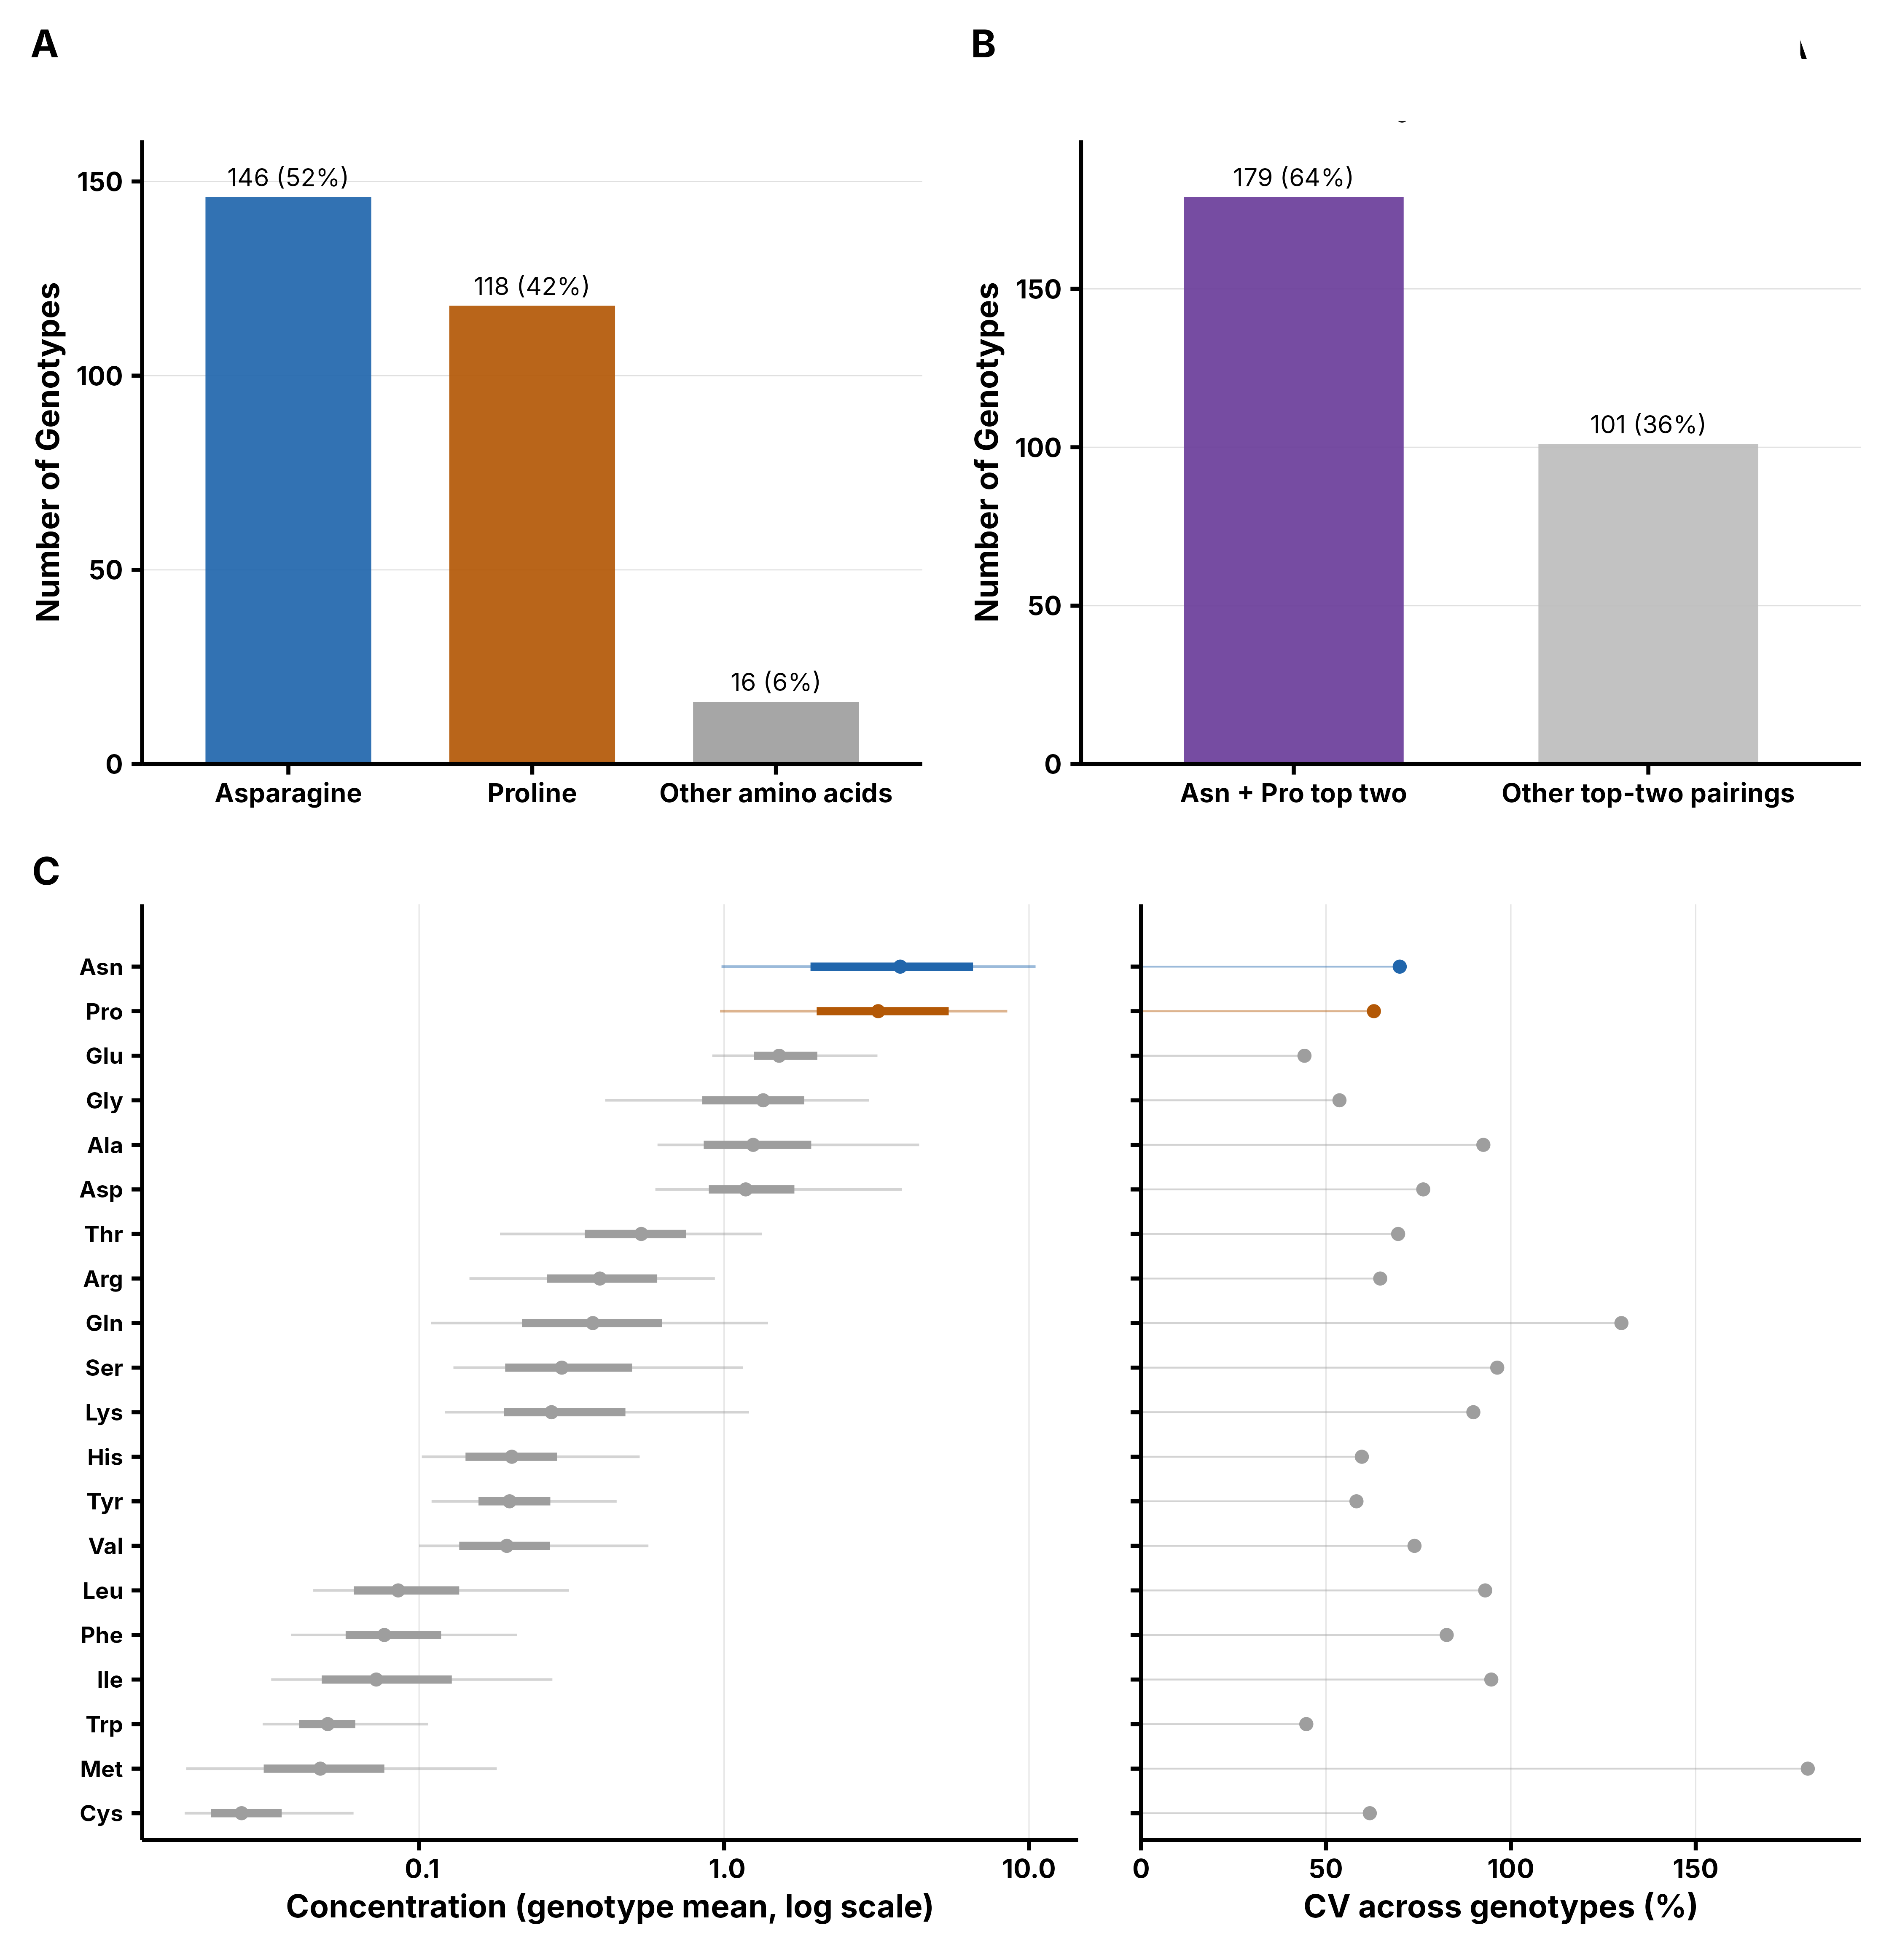
\includegraphics[width=0.95\textwidth]{final/supp_figs/SuppFig1_FAA_composition.png}
    \caption{\textbf{Free amino acid composition of the Goodman--Buckler panel.}
    \textbf{(A)}, Number of genotypes in which each free amino acid ranked most abundant,
    based on genotype means across four replicates ($n = 280$ genotypes).
    \textbf{(B)}, Number of genotypes in which Asn and Pro together occupied the
    top two ranks, in either order.
    \textbf{(C)}, Abundance and variability of each free amino acid. Left, concentration per
    genotype mean on a log scale: point, median across genotypes; thick bar, interquartile
    range; thin bar, 5th--95th percentile; amino acids ordered by median. Right,
    coefficient of variation across genotypes for the same ordering. Asn is shown in blue and Pro in orange throughout.}
    \label{fig:supp_faa_asn_pro_rank}
\end{figure*}

% =========================
% SUPP FIGURE S2
% =========================  

\begin{figure*}[ht!]
    \centering
    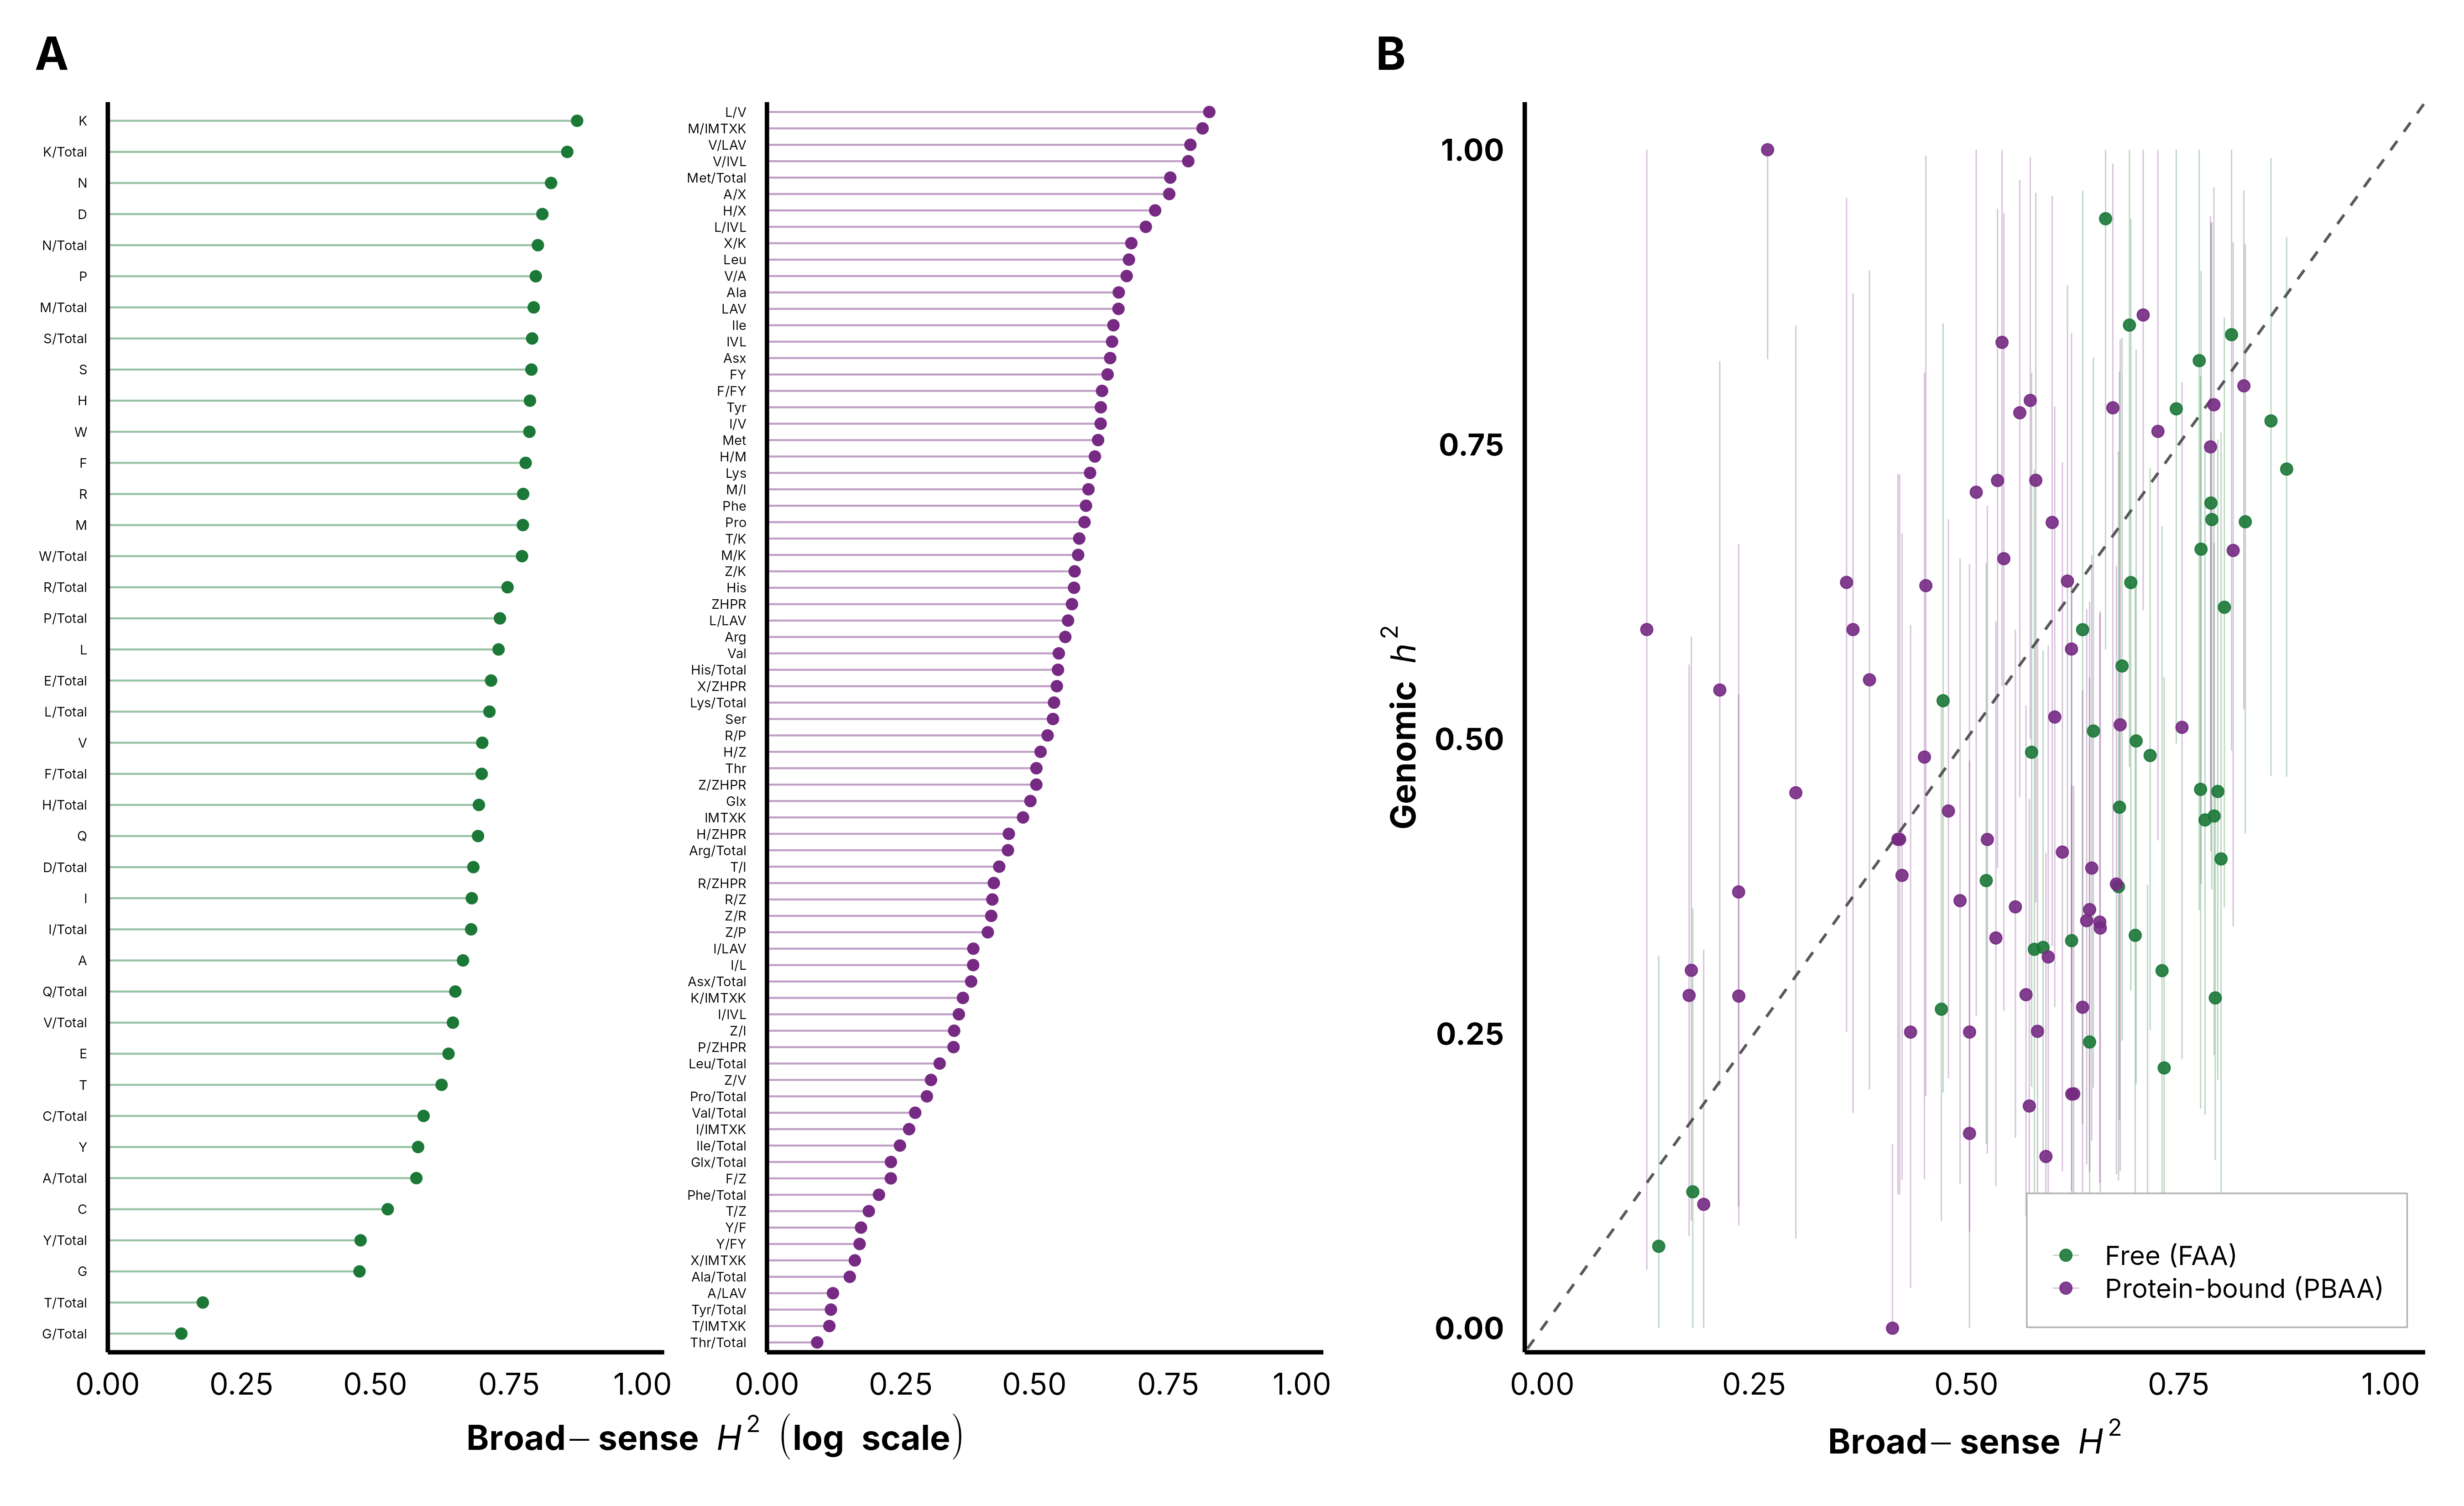
\includegraphics[width=\textwidth]{final/supp_figs/SuppFig2_heritability.png}
    \caption{\textbf{Heritability of grain amino acid phenotypes in the Goodman--Buckler panel.}
    \textbf{(A)}, Broad-sense heritability $H^2$ on a line-mean basis shown for 40 free and 76 protein-bound amino acid traits.
    \textbf{B}, Genomic heritability $h^2$ from a VanRaden genomic relationship matrix plotted against $H^2$, with error bars giving the 95\% profile-likelihood interval on $h^2$ and the dashed line showing $y = x$. Fifteen of
    116 traits returned a non-zero $h^2$ from a permuted phenotype and are excluded from
    panel \textbf{B}; their $H^2$ is unaffected and is retained in panel \textbf{A}.}
    \label{fig:supp_heritability}
\end{figure*}

% =========================
% SUPP FIGURE S3
% =========================
\begin{figure*}[ht!]
    \centering
    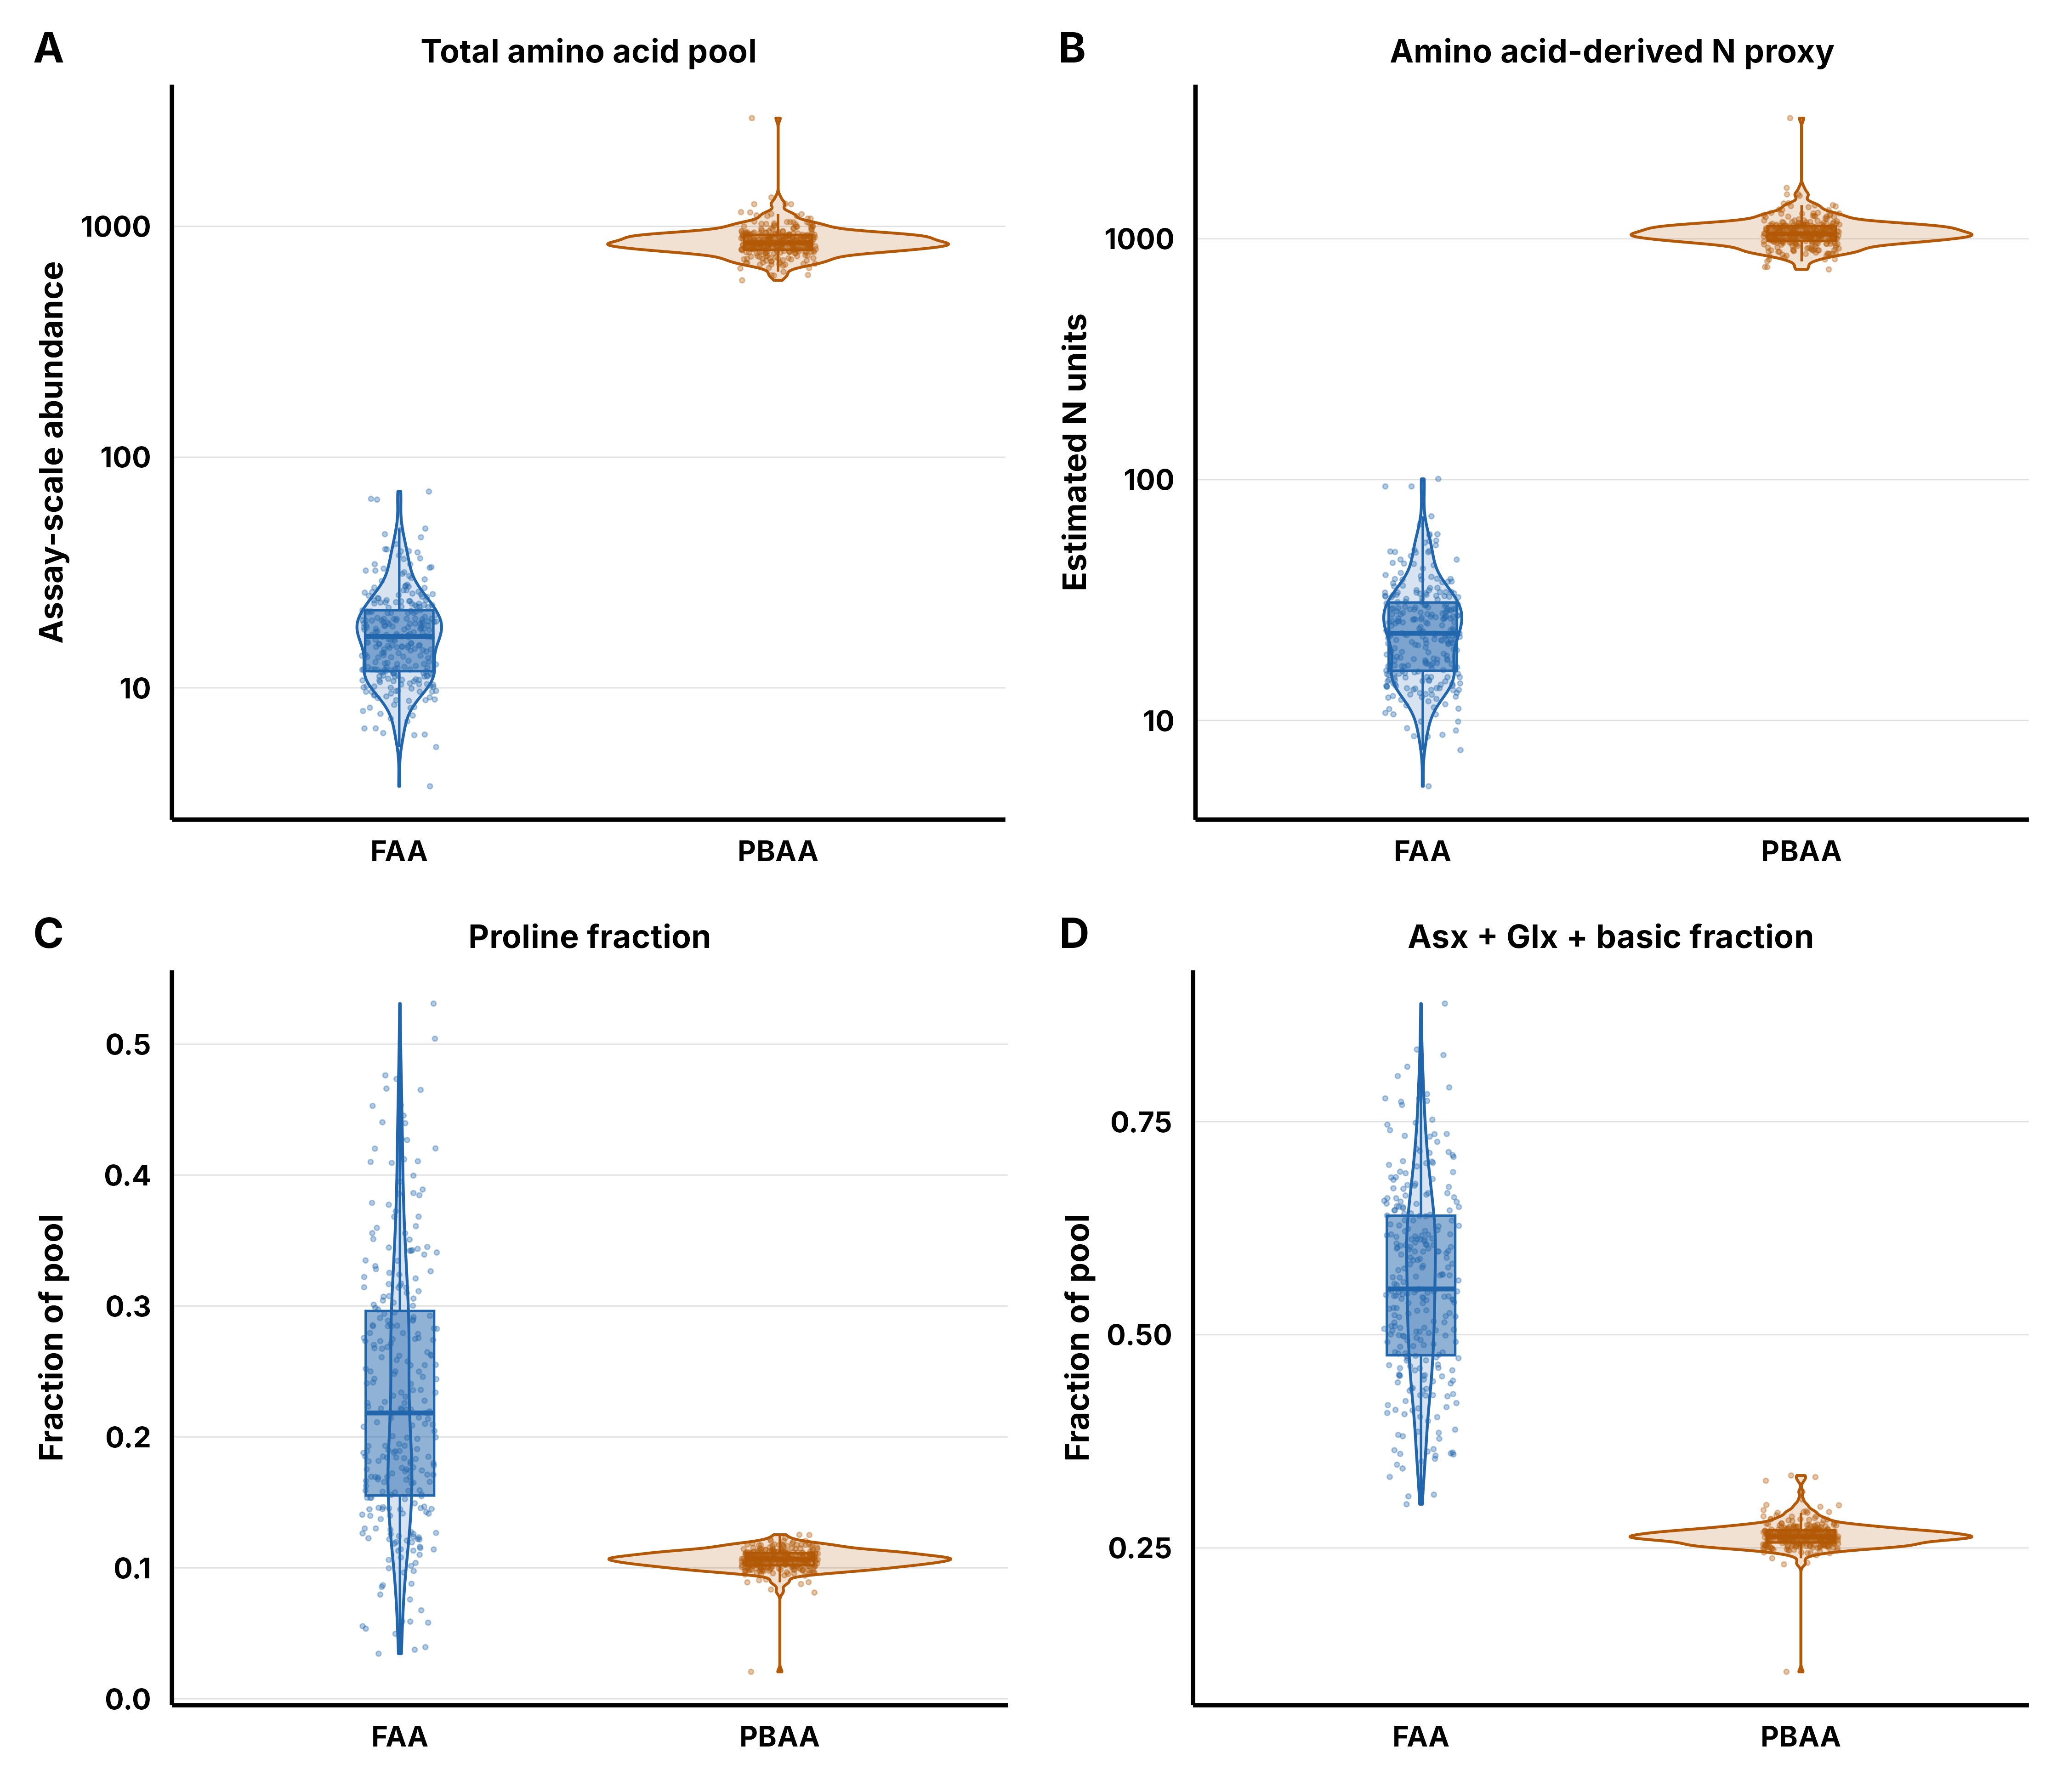
\includegraphics[width=\textwidth]{final/supp_figs/SuppFig3_FAA_vs_PBAA_pools.png}
    \caption{\textbf{Free (FAA) and protein-bound (PBAA) amino acid pools across matched Goodman--Buckler lines ($n = 279$)}. \textbf{(A)}, Total amino acid pool. \textbf{(B)}, Amino acid-derived N proxy, with each amino acid weighted by its number of N atoms (Asx and Glx, unresolved after acid
    hydrolysis, at 1.5 N). \textbf{(C)}, Proline fraction. \textbf{(D)}, Asx + Glx + basic
    (Arg, Lys, His) fraction. Fractions use matched denominators: free Asp + Asn and Glu + Gln
    are combined, and glycine, tryptophan and cysteine are excluded from the free-pool total. Violins show the distribution across lines and boxes the median and interquartile range.}
    \label{fig:supp_gb_faa_pbaa_metrics}
\end{figure*}

% =========================
% SUPP FIGURE S4
% =========================
\begin{figure*}[ht!]
    \centering
    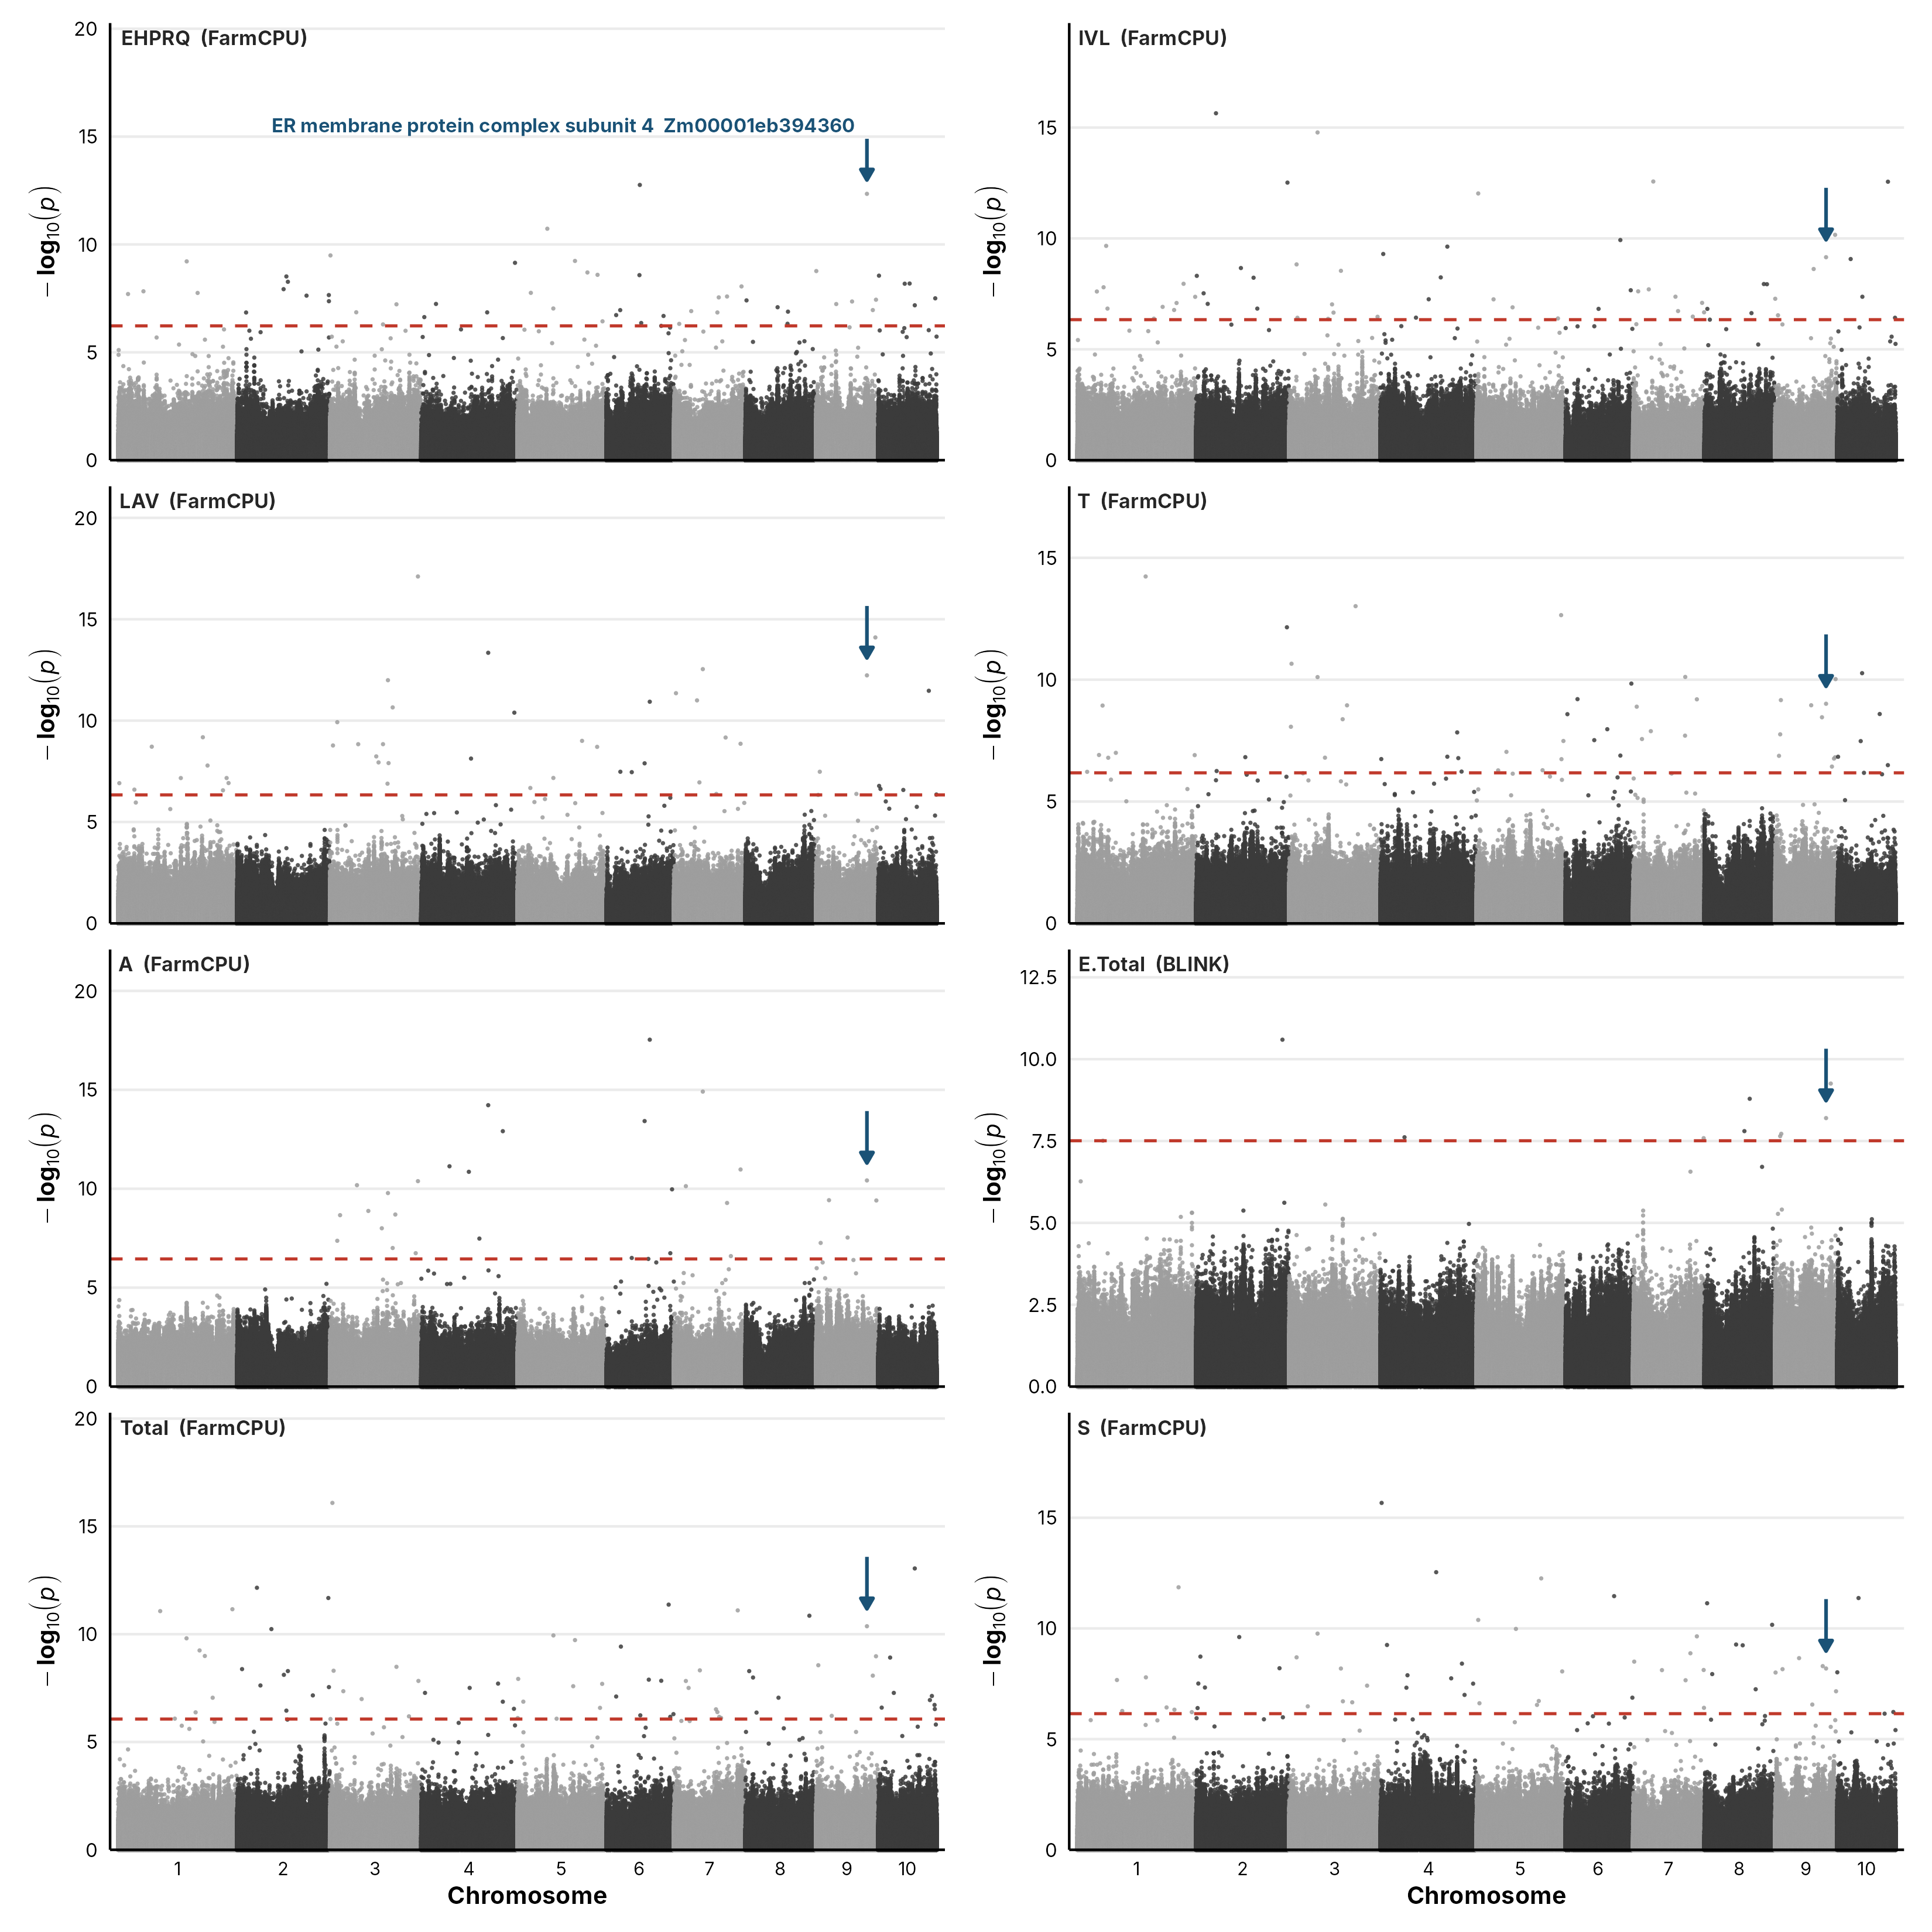
\includegraphics[width=0.82\textwidth]{final/supp_figs/SuppFig_amino_chr9_locus_manhattan.png}
    \caption{\textbf{Manhattan plots for a locus on chromosome 9 associated with nine amino acid phenotypes.} Eight phenotypes had an FDR-significant association near \textit{Zm00001eb394360} (ER membrane protein complex subunit 4; chr9:133,919,123--133,923,877); \textit{N.E} ($P = 1.1 \times 10^{-7}$) is omitted. Four SNPs spanning 13 kb, from the 3$'$ end of \textit{Zm00001eb394360} to the 5$'$ end of \textit{Zm00001eb394380} (rhomboid-like protein 19), are significant for \textit{A}, \textit{LAV}, \textit{IVL}, \textit{T}, \textit{S}, \textit{Total} and \textit{E.Total}, and two further SNPs are significant for \textit{EHPRQ} and \textit{N.E}. Dashed red lines indicate the 5\% Benjamini--Hochberg FDR threshold. The model for each phenotype is in parentheses.}
    \label{fig:supp_amino_chr9_locus}
\end{figure*}

% =========================
% SUPP FIGURE S5
% =========================
\begin{figure*}[ht!]
  \centering
  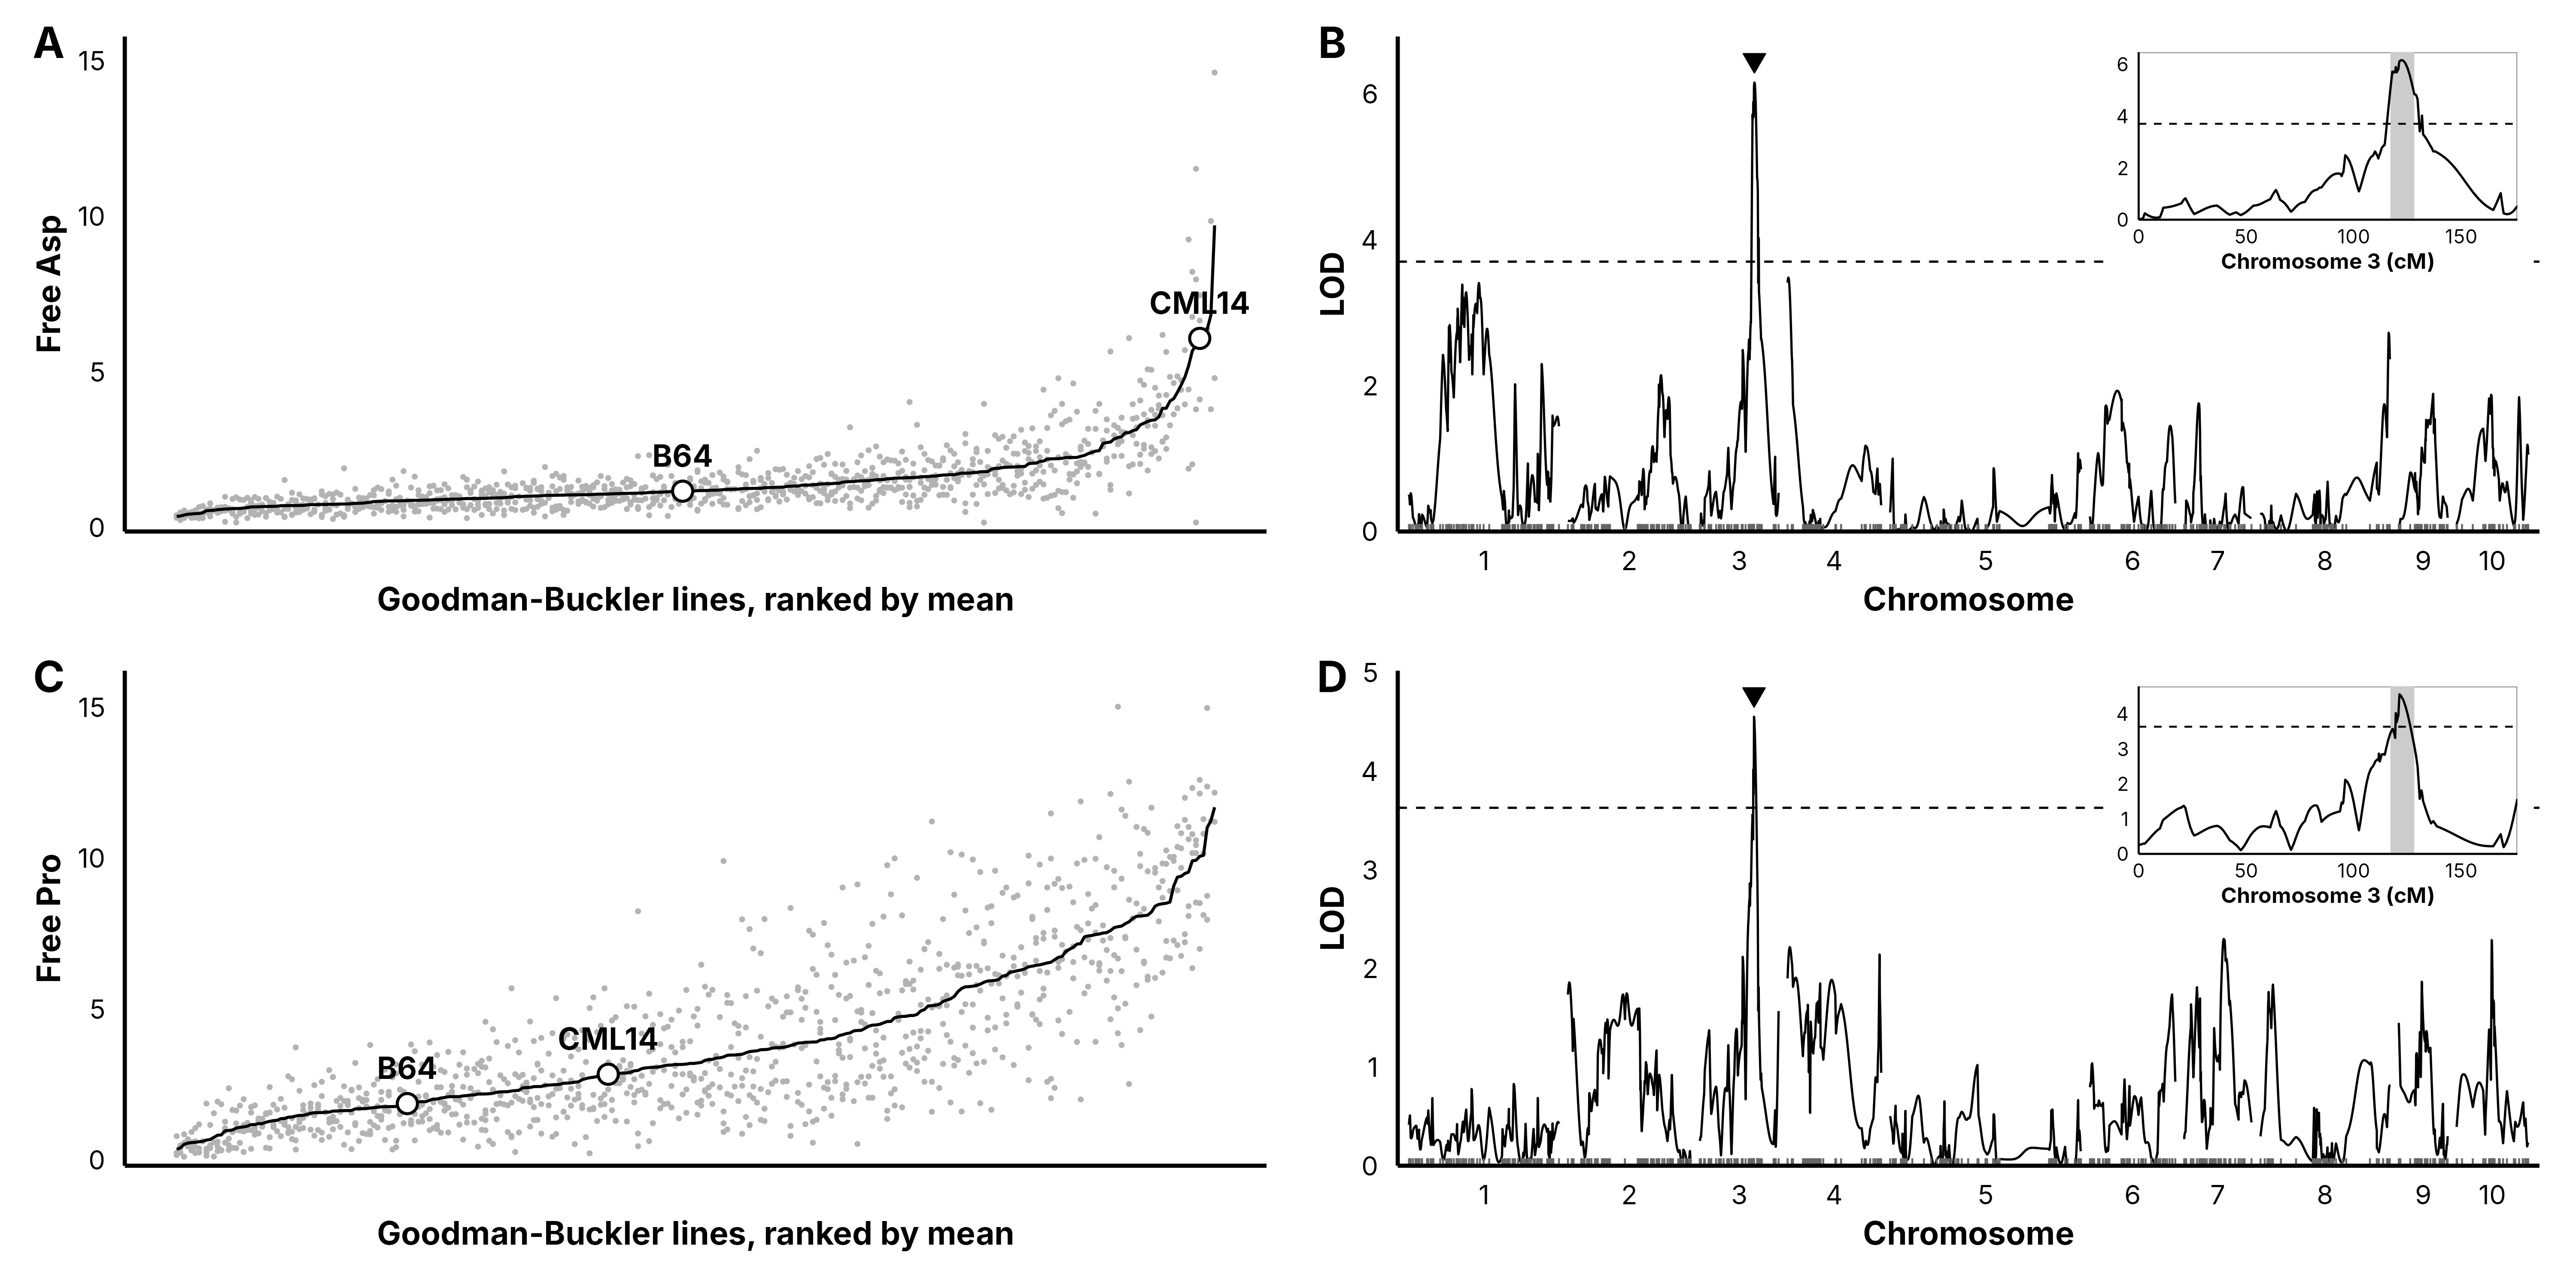
\includegraphics[width=\textwidth]{final/supp_figs/SuppFig_QTL_Asp_Pro_panel.png}
  \caption{\textbf{Free Asp and Pro map to the same QTL on chromosome 3 in the B64 $\times$ CML14 population.} \textbf{(A, C)} Free Asp (A) and Pro (C) in the Goodman--Buckler panel (nmol~$\mu$g$^{-1}$), with lines ranked by their mean. Open circles mark B64 and CML14. \textbf{(B, D)} Genome-wide LOD scores for free Asp (B) and Pro (D) in the B64 $\times$ CML14 F$_{2:3}$ population. Dashed lines show the genome-wide threshold ($\alpha = 0.05$, 1,000 permutations). The triangle marks the chromosome 3 peak, and the inset shows chromosome 3 with the overlap of the Asp and Pro 1.5-LOD support intervals shaded.}
  \label{suppfig:qtl_asp_pro}
\end{figure*}


% =========================
% SUPP FIGURE S6
% =========================
\begin{figure}[htbp]
  \centering
  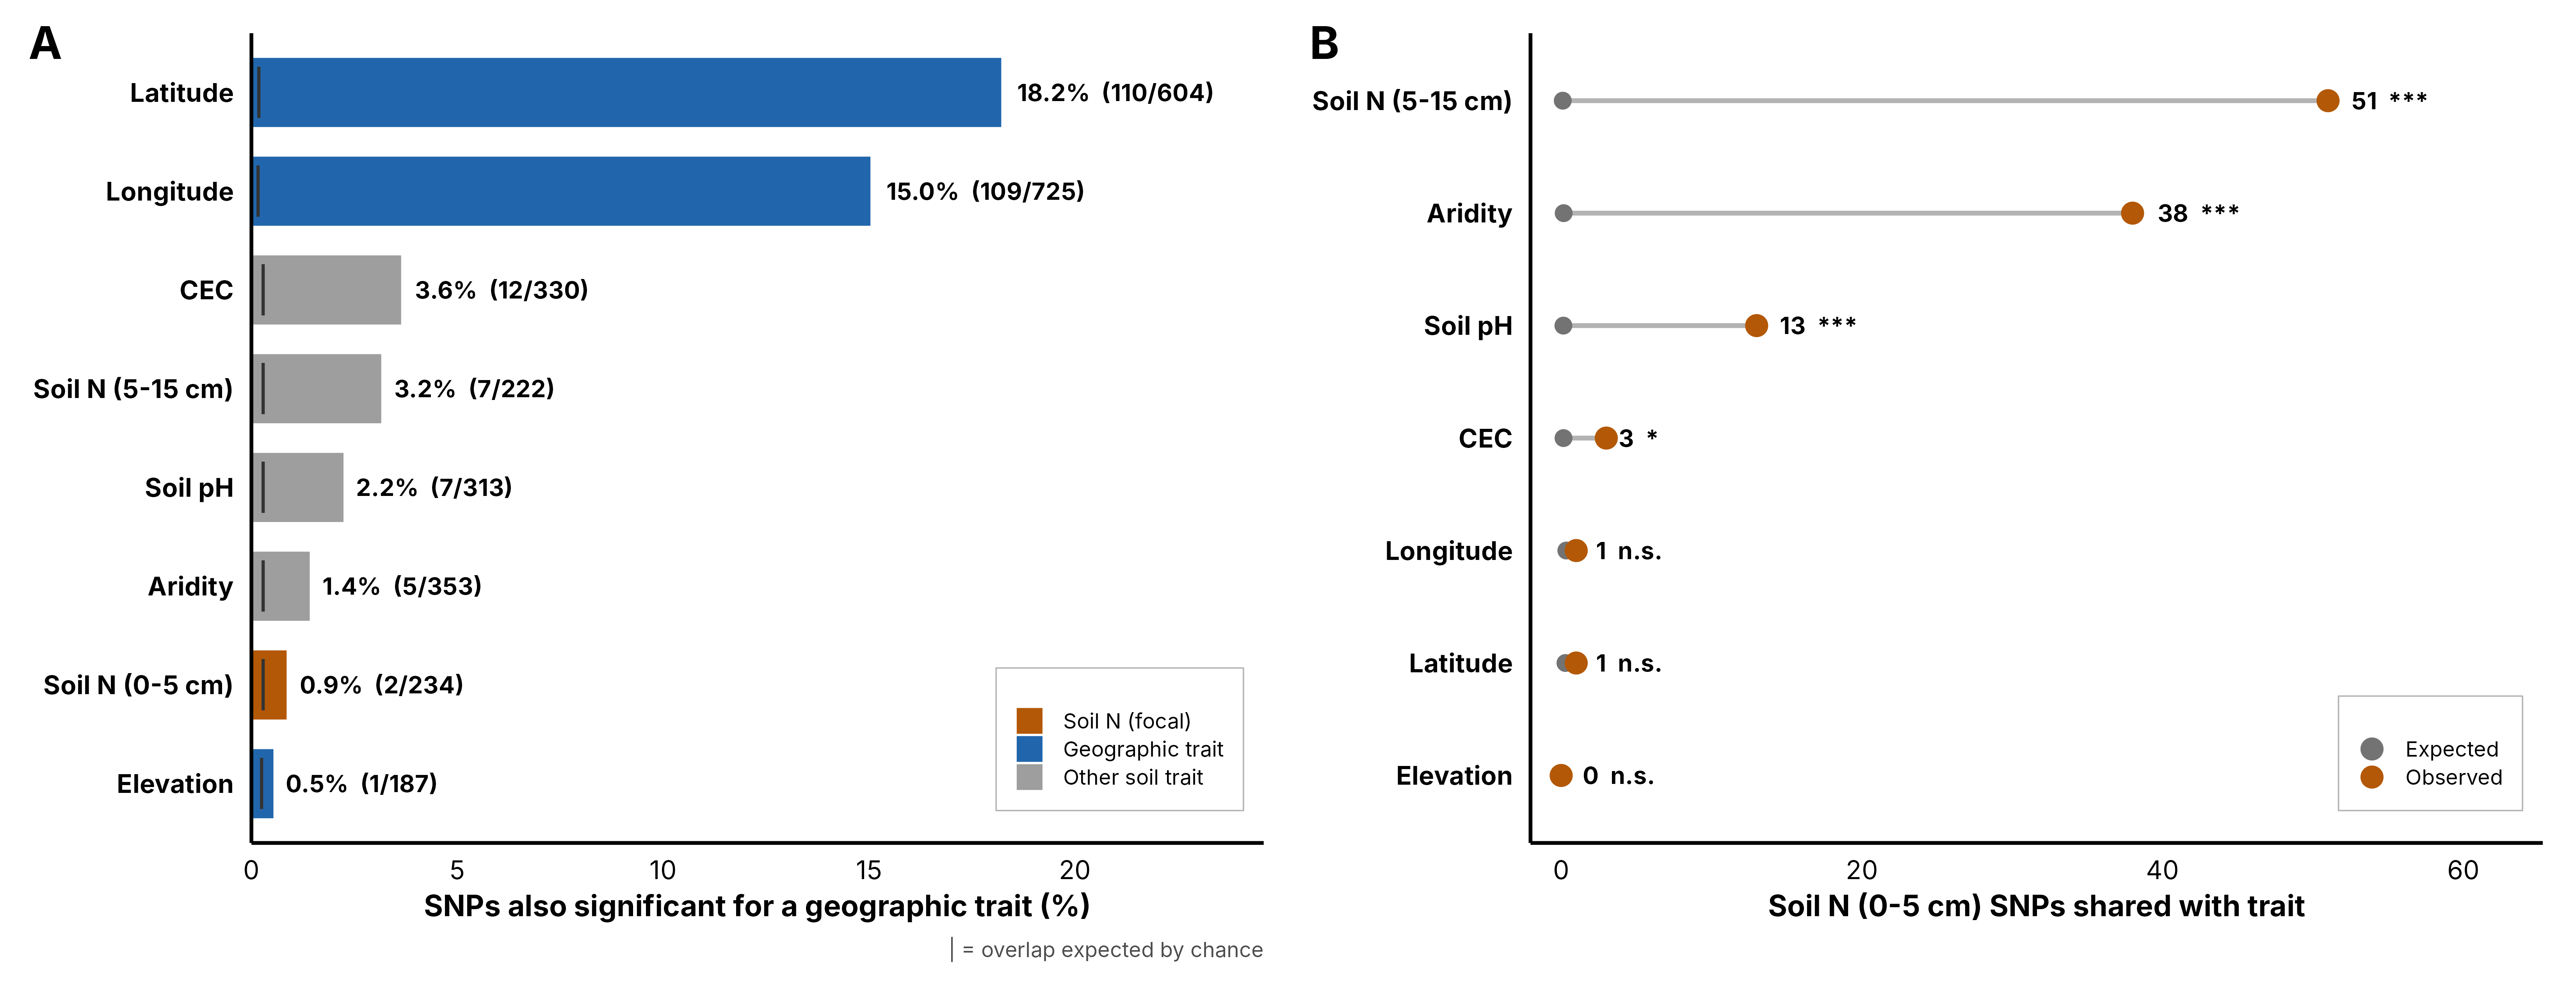
\includegraphics[width=\textwidth]{final/supp_figs/SuppFig_soilN_specificity.png}
  \caption{\textbf{Overlap of soil-N associations with other environmental GWAS.}
  Each variable was scanned with MLM, BLINK and FarmCPU; a SNP counts as
  significant for a variable if it reaches 5\% FDR in any model.
  \textbf{(A)} Percentage of each variable's significant SNPs that are also significant for a
  geographic variable (latitude, longitude, elevation; the variable itself excluded). Vertical
  ticks, percentage expected by chance.
  \textbf{(B)} SNPs shared between soil N (0--5~cm) and each other variable: observed (orange)
  vs.\ expected (grey). One-sided hypergeometric test, $M = 495{,}755$:
  *\,$P<0.05$; **\,$P<10^{-5}$; ***\,$P<10^{-20}$; n.s., not significant.
  }
  \label{suppfig:soilN_specificity}
\end{figure}


% =========================
% SUPP FIGURE S7
% =========================                                                    

\begin{figure}[htbp]
  \centering
  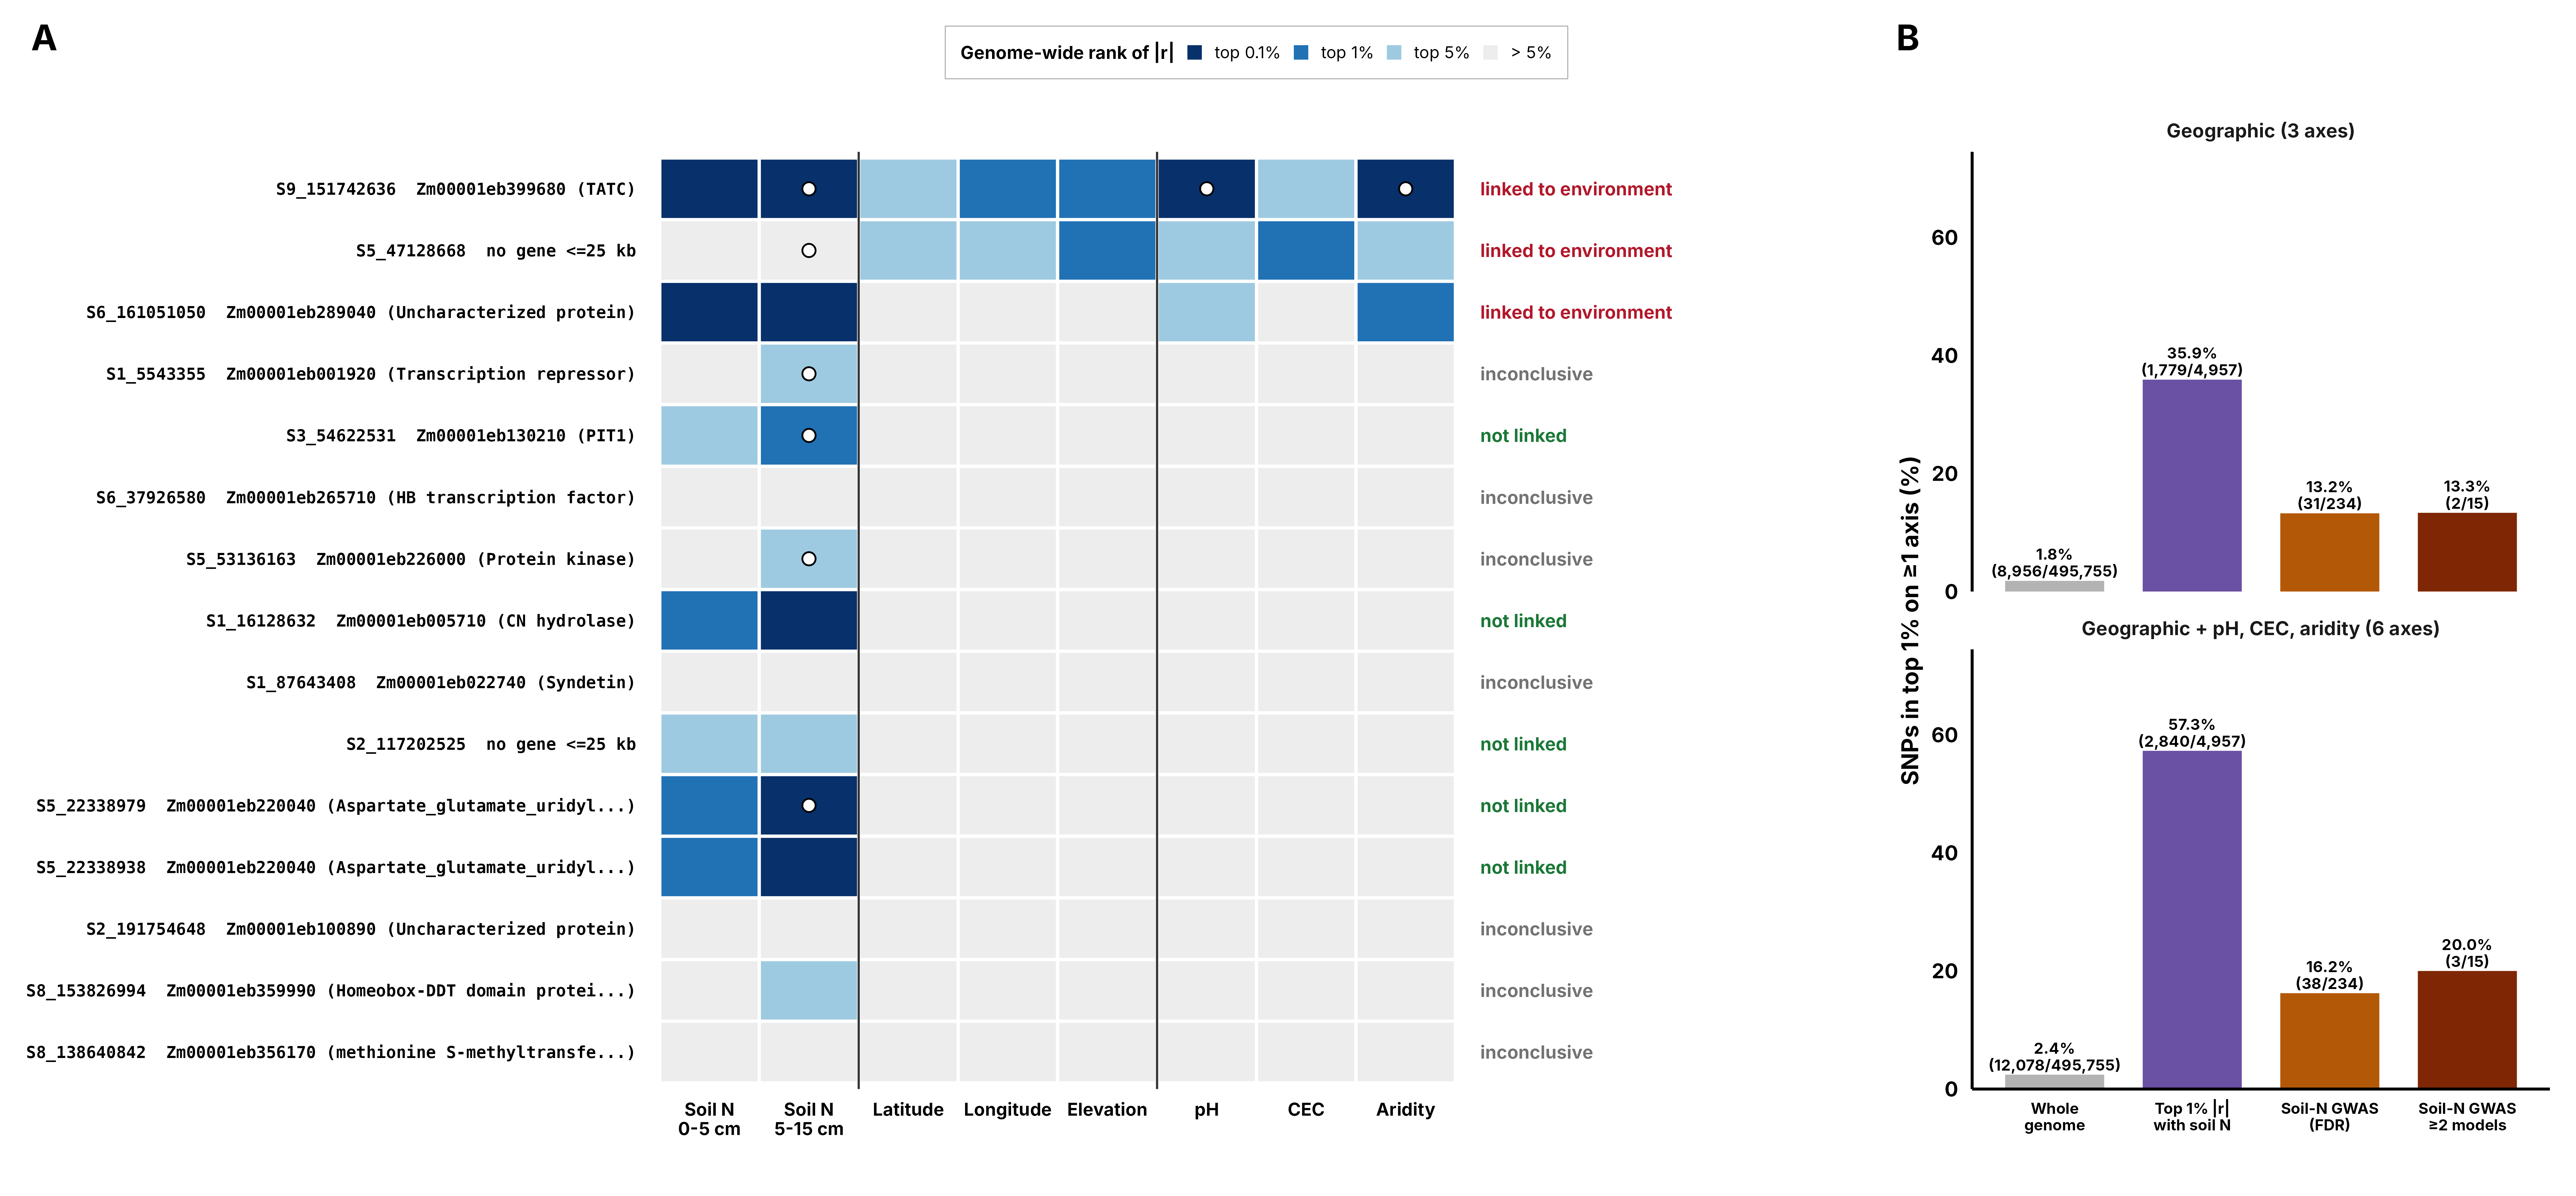
\includegraphics[width=\textwidth]{final/supp_figs/SuppFig_soilN_geno_env_correlation.png}
  \caption{\textbf{Genotype--environment correlation test for the soil-N SNPs.}
  We computed the Pearson correlation ($r$) between the SNP's genotype
  (0, 1 or 2 copies of the allele) and each site variable across 3,107 accessions, then ranked
  every SNP against the whole genome by $|r|$ (e.g.\ ``top 1\%'' = fewer than 1\% of SNPs
  correlate more strongly with that variable).
  \textbf{(A)} The 15 soil-N SNPs significant in at least two GWAS models. Tile color shows the
  genome-wide rank of each SNP's correlation with each variable. Open circles mark SNPs that were
  also significant (5\% FDR) in that variable's own GWAS. Each SNP's call is shown on the right:
  \textit{linked to environment}, its genotype is in the top 1\% of the genome for correlation
  with at least one non-N variable, so its soil-N association cannot be separated from geography
  or climate;
  \textit{not linked}, its genotype correlates strongly with soil N (top 5\%) but not with any
  other variable;
  \textit{inconclusive}, its genotype correlates only weakly with soil N across all accessions
  (outside the top 5\%), so there is no soil-N correlation to compare the other variables
  against. These SNPs were detected only by BLINK and FarmCPU, which test each SNP after
  accounting for population structure and other strongly associated SNPs; this test applies no
  such adjustment and therefore cannot judge them in either direction.
  \textbf{(B)} Expectation test: percentage of SNPs whose genotype is in the top 1\% for at least
  one geographic variable (latitude, longitude, elevation; top) or for at least one of all six
  non-N variables (bottom), for the whole genome, for SNPs in the top 1\% for correlation with
  soil N, and for the soil-N GWAS SNPs.}
  \label{suppfig:soilN_geno_env}
\end{figure}

% =========================
% SUPP FIGURE S8
% =========================
\begin{figure*}[!htbp]
    \centering
    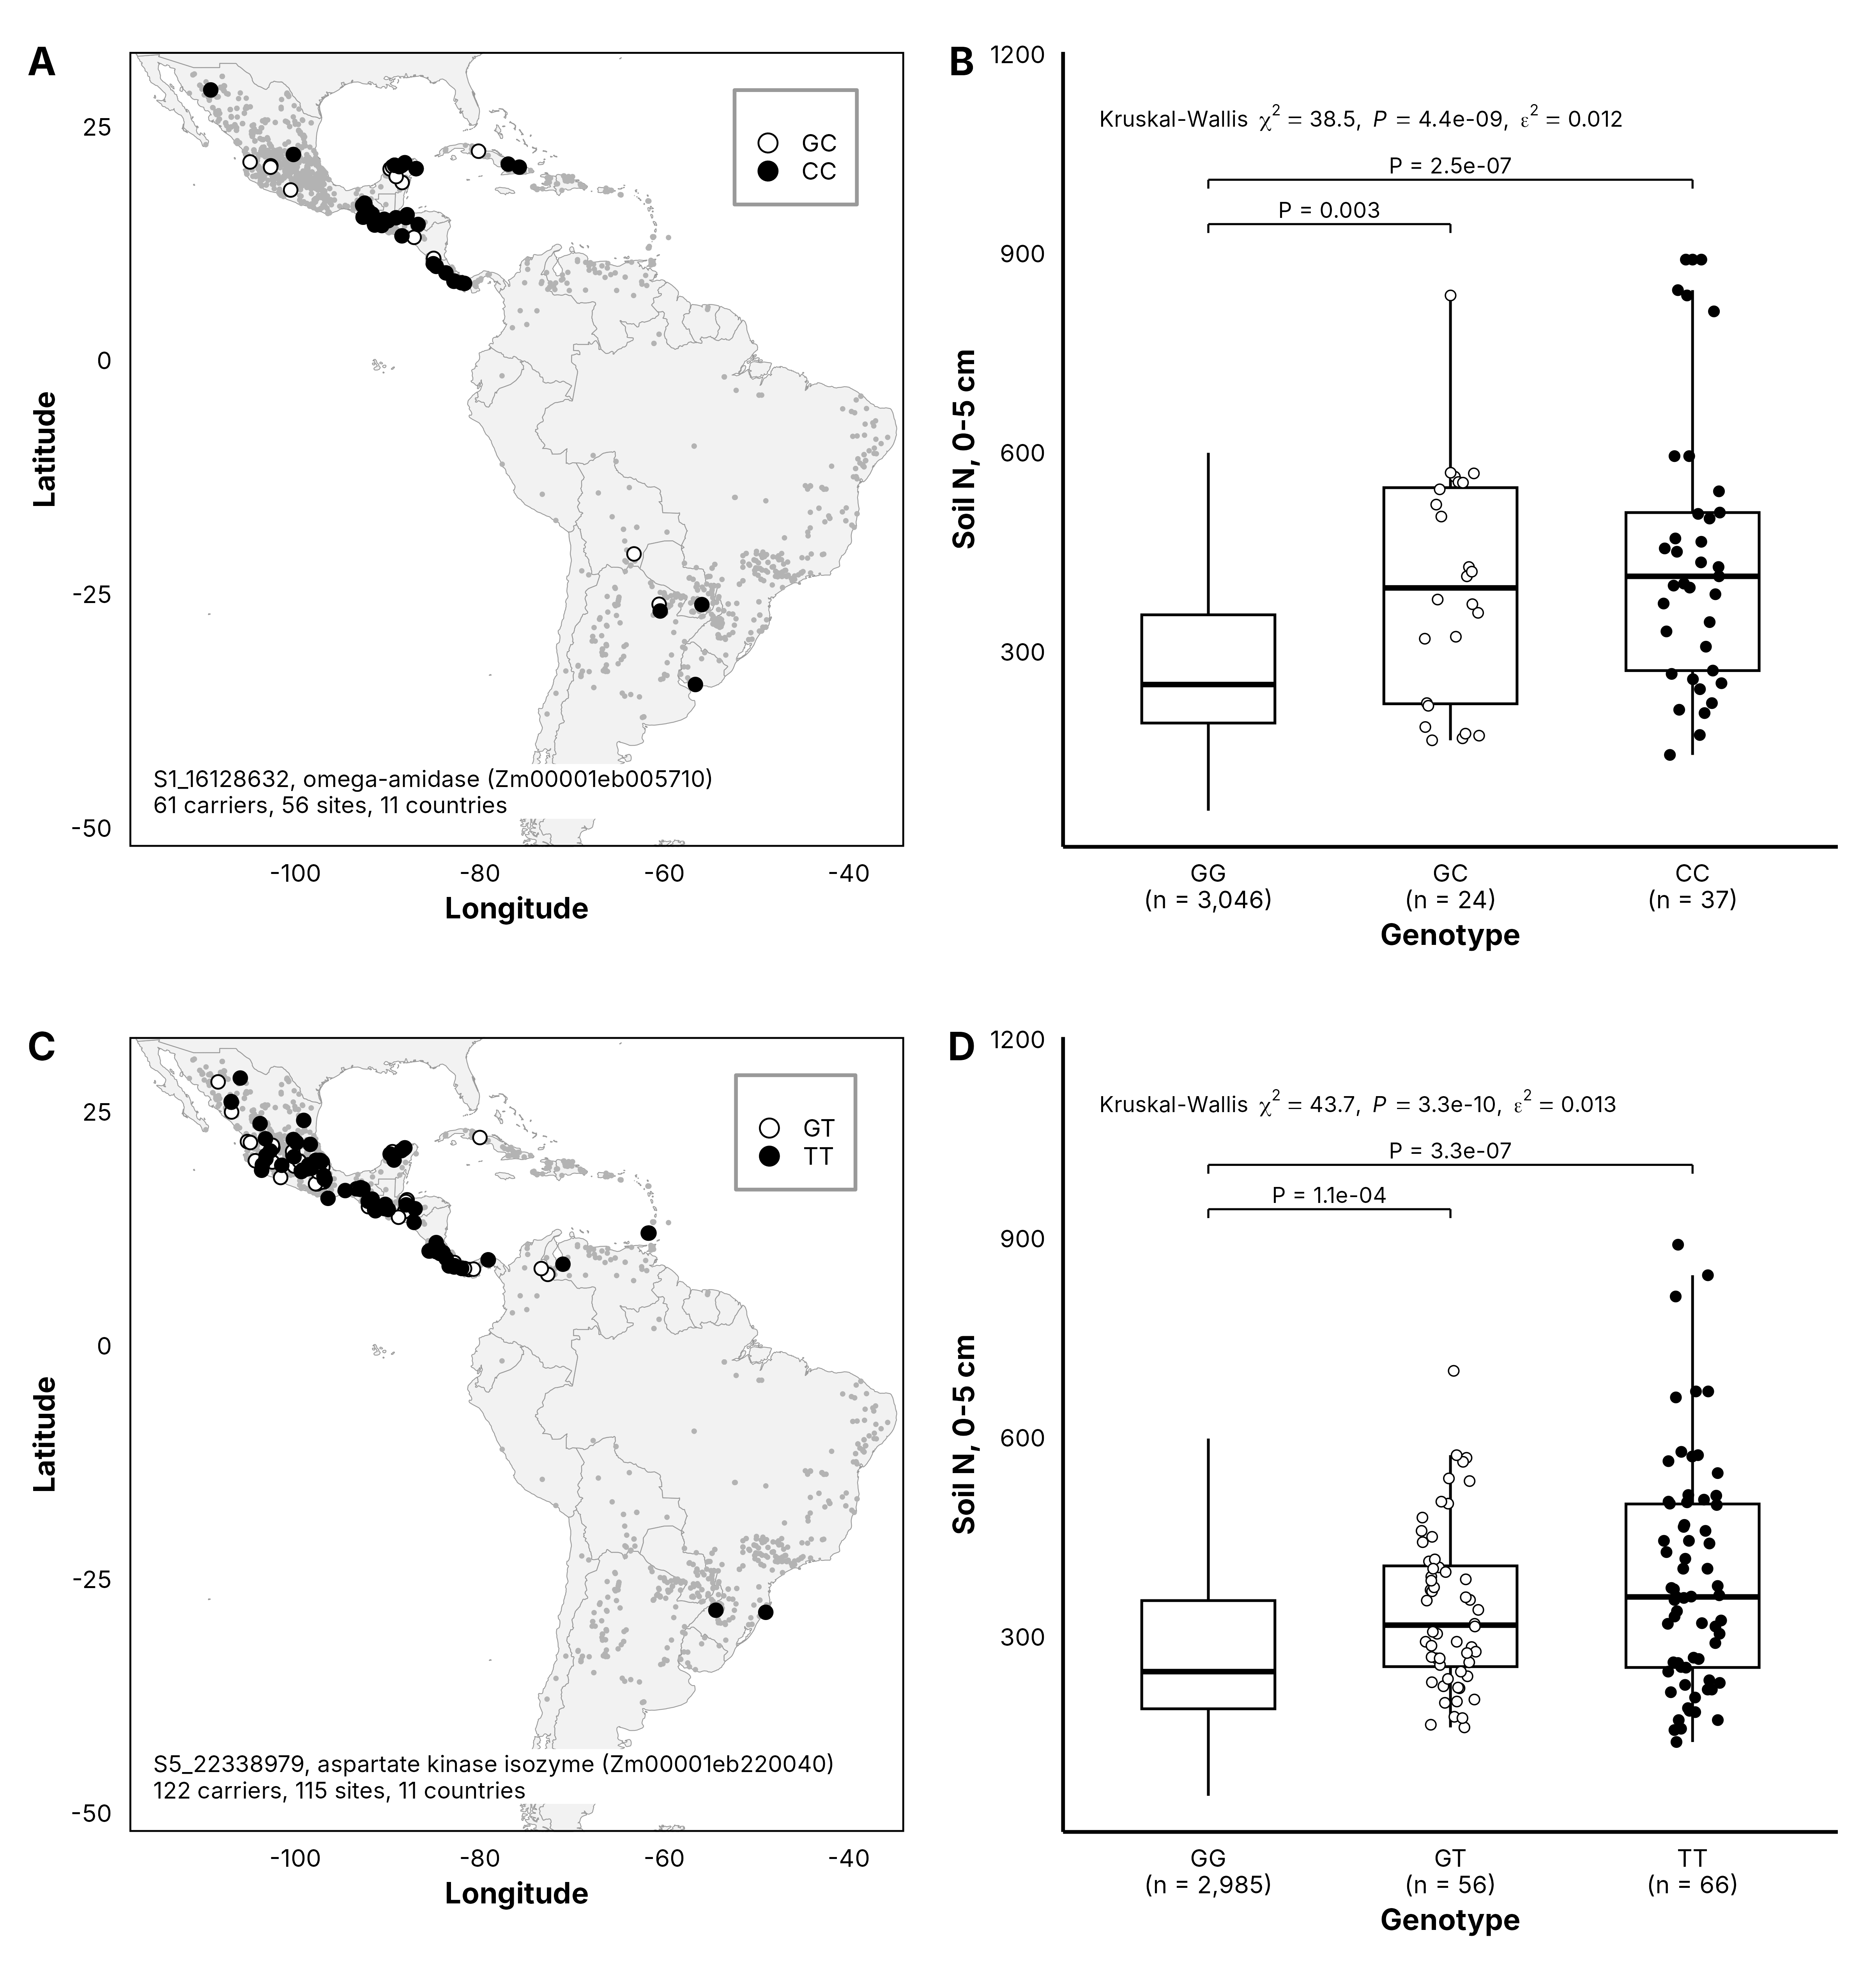
\includegraphics[width=0.85\textwidth]{final/supp_figs/SuppFig_soilN_focal_allele_geography.png}
    \caption{\textbf{Geography and soil N of the two focal soil-N SNPs.} \textbf{(A, B)} S1\_16128632 in the $\omega$-amidase gene \textit{Zm00001eb005710}. \textbf{(C, D)} S5\_22338979 near the aspartate kinase isozyme gene \textit{Zm00001eb220040}. \textbf{(A, C)} Collection sites of the 3,107 landraces. Grey, homozygous for the major allele; white, heterozygous; black, homozygous for the minor allele. Numbers of carriers, independent collection sites, and countries are given in each panel. \textbf{(B, D)} Soil N at 0--5 cm by genotype. Boxes show the median and interquartile range, and points show individual values. Differences among genotypes were tested with a Kruskal--Wallis test ($\varepsilon^2$, effect size), followed by Dunn tests with Holm correction, and only significant pairwise comparisons are shown.}
    \label{suppfig:soilN_focal_geography}
\end{figure*}


% =========================
% SUPP FIGURE S9
% =========================
\begin{figure*}[htbp]
\centering
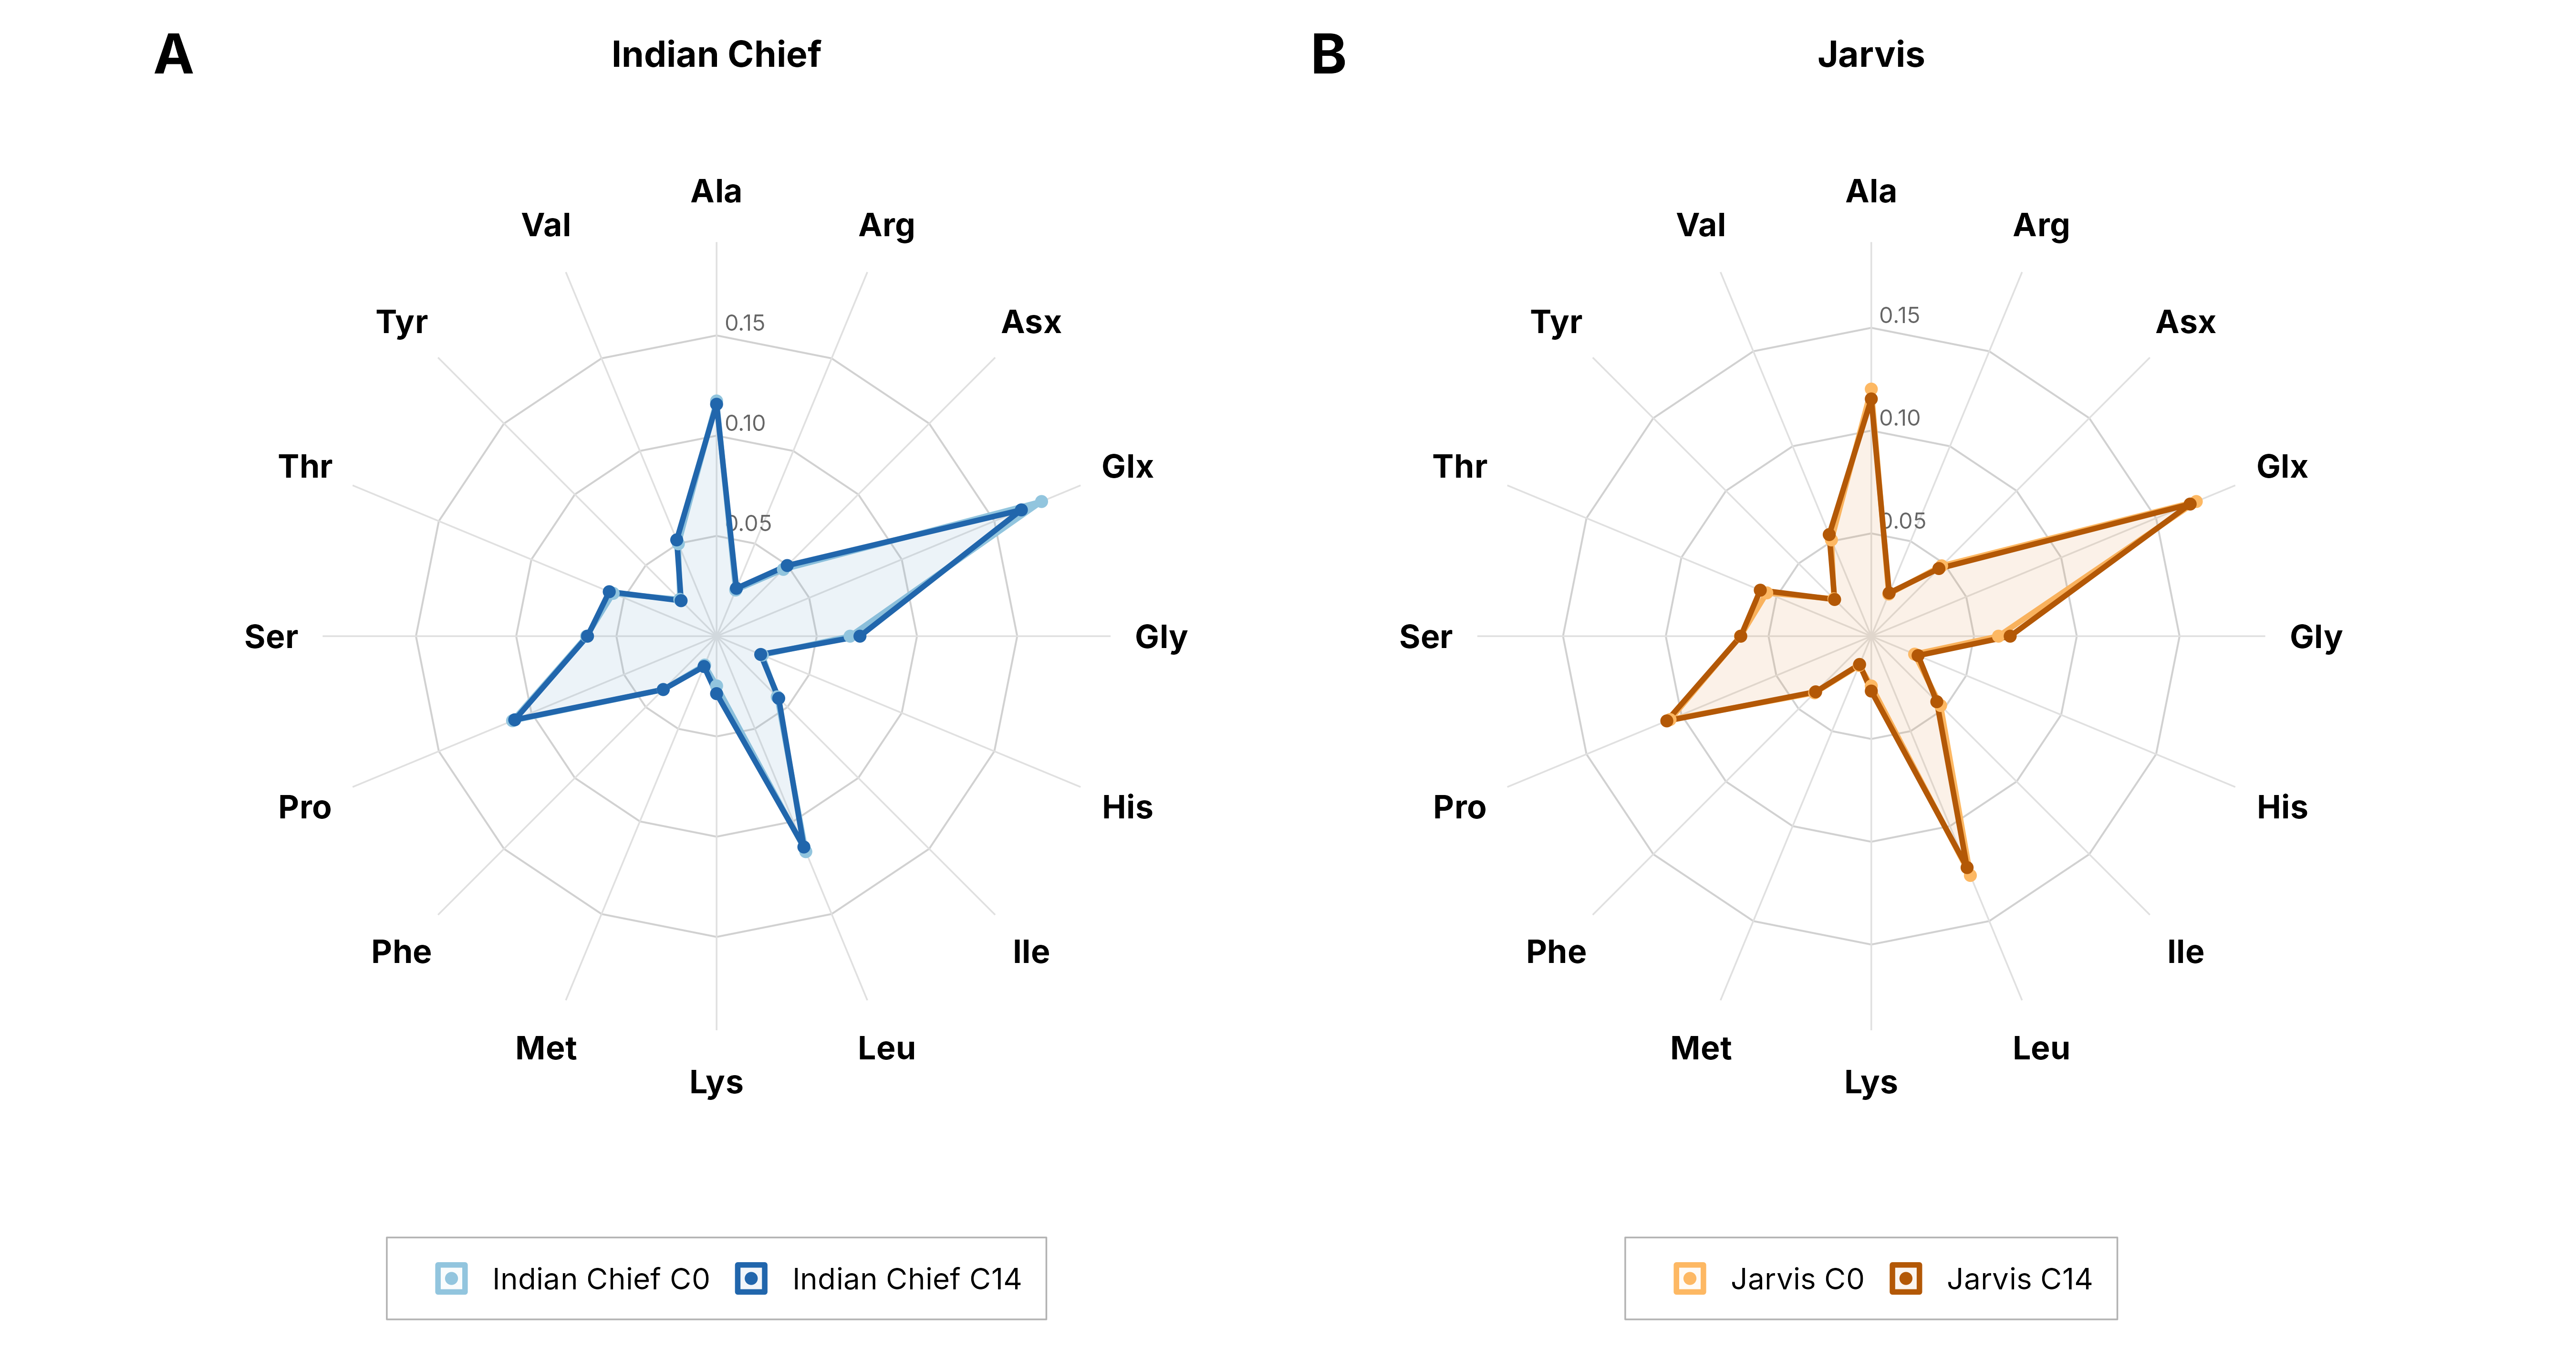
\includegraphics[width=\textwidth]{final/supp_figs/SuppFig_IC_J_PBAA_composition.png}
\caption{
\textbf{Protein-bound amino acid (PBAA) composition in Indian Chief and Jarvis at Cycle 0 (C0) and Cycle 14 (C14).} Mean fraction of each of 16 PBAA in the total PBAA pool, averaged over biological samples, for \textbf{(A)} Indian Chief and \textbf{(B)} Jarvis. Asx and Glx are the combined Asp + Asn and Glu + Gln pools after acid hydrolysis; tryptophan and cysteine are not measured. Rings mark fractions of 0.05, 0.10 and 0.15. No amino acid differed between cycles in either population (two-sided Wilcoxon rank-sum tests, Benjamini--Hochberg-adjusted across the 16 amino acids.
}
\label{fig:supp_pbaa_profiles}
\end{figure*}

% =========================
% SUPP FIGURE S10
% =========================
\begin{figure*}[htbp]
\centering
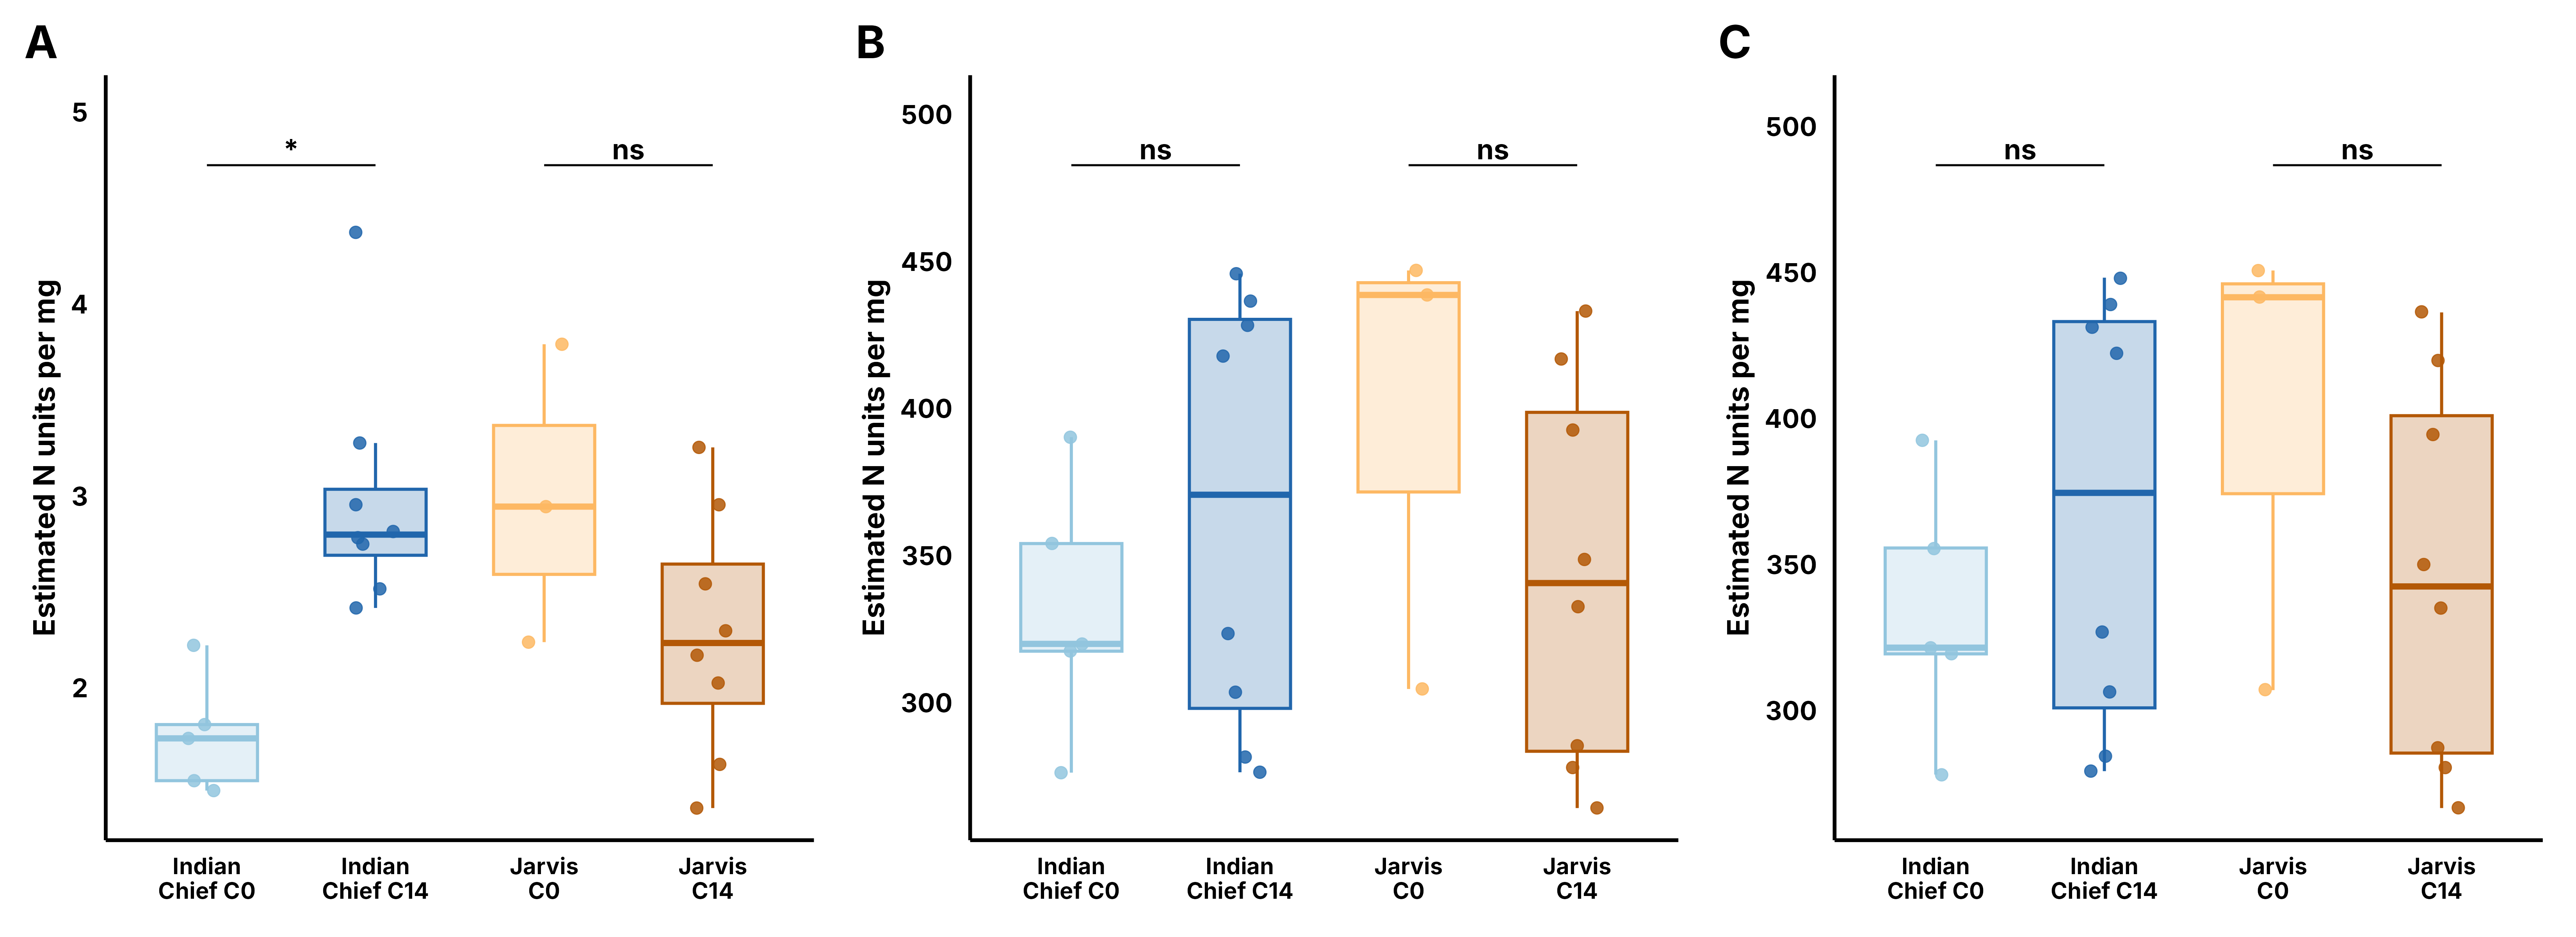
\includegraphics[width=\textwidth]{final/supp_figs/SuppFig_IC_J_AA_N_pools.png}
\caption{
\textbf{Amino acid-derived nitrogen per mg sample in Indian Chief and Jarvis at Cycle 0 (C0) and Cycle~14 (C14).} \textbf{(A)} FAA-derived N, \textbf{(B)} estimated protein-bound amino acid-derived N and \textbf{(C)} estimated total amino acid-derived N (A + B). Each amino acid was weighted by its number of N atoms (Arg 4; His 3; Asn, Gln, Lys and Trp 2; all others 1; protein-bound Asx and Glx 1.5) and divided by sample mass. Points are biological samples (Indian Chief C0 $n = 5$, C14 $n = 8$; Jarvis C0 $n = 3$, C14 $n = 8$); boxes show the median and interquartile range. Brackets show within-population two-sided Wilcoxon rank-sum tests, Benjamini--Hochberg-adjusted across the three measures: * adjusted $P < 0.05$; ns, not significant.
}
\label{fig:supp_ic_j_aa_n_pools}
\end{figure*}

% =========================
% SUPP FIGURE S11
% =========================                                                  
\begin{figure*}[!htbp]
    \centering
    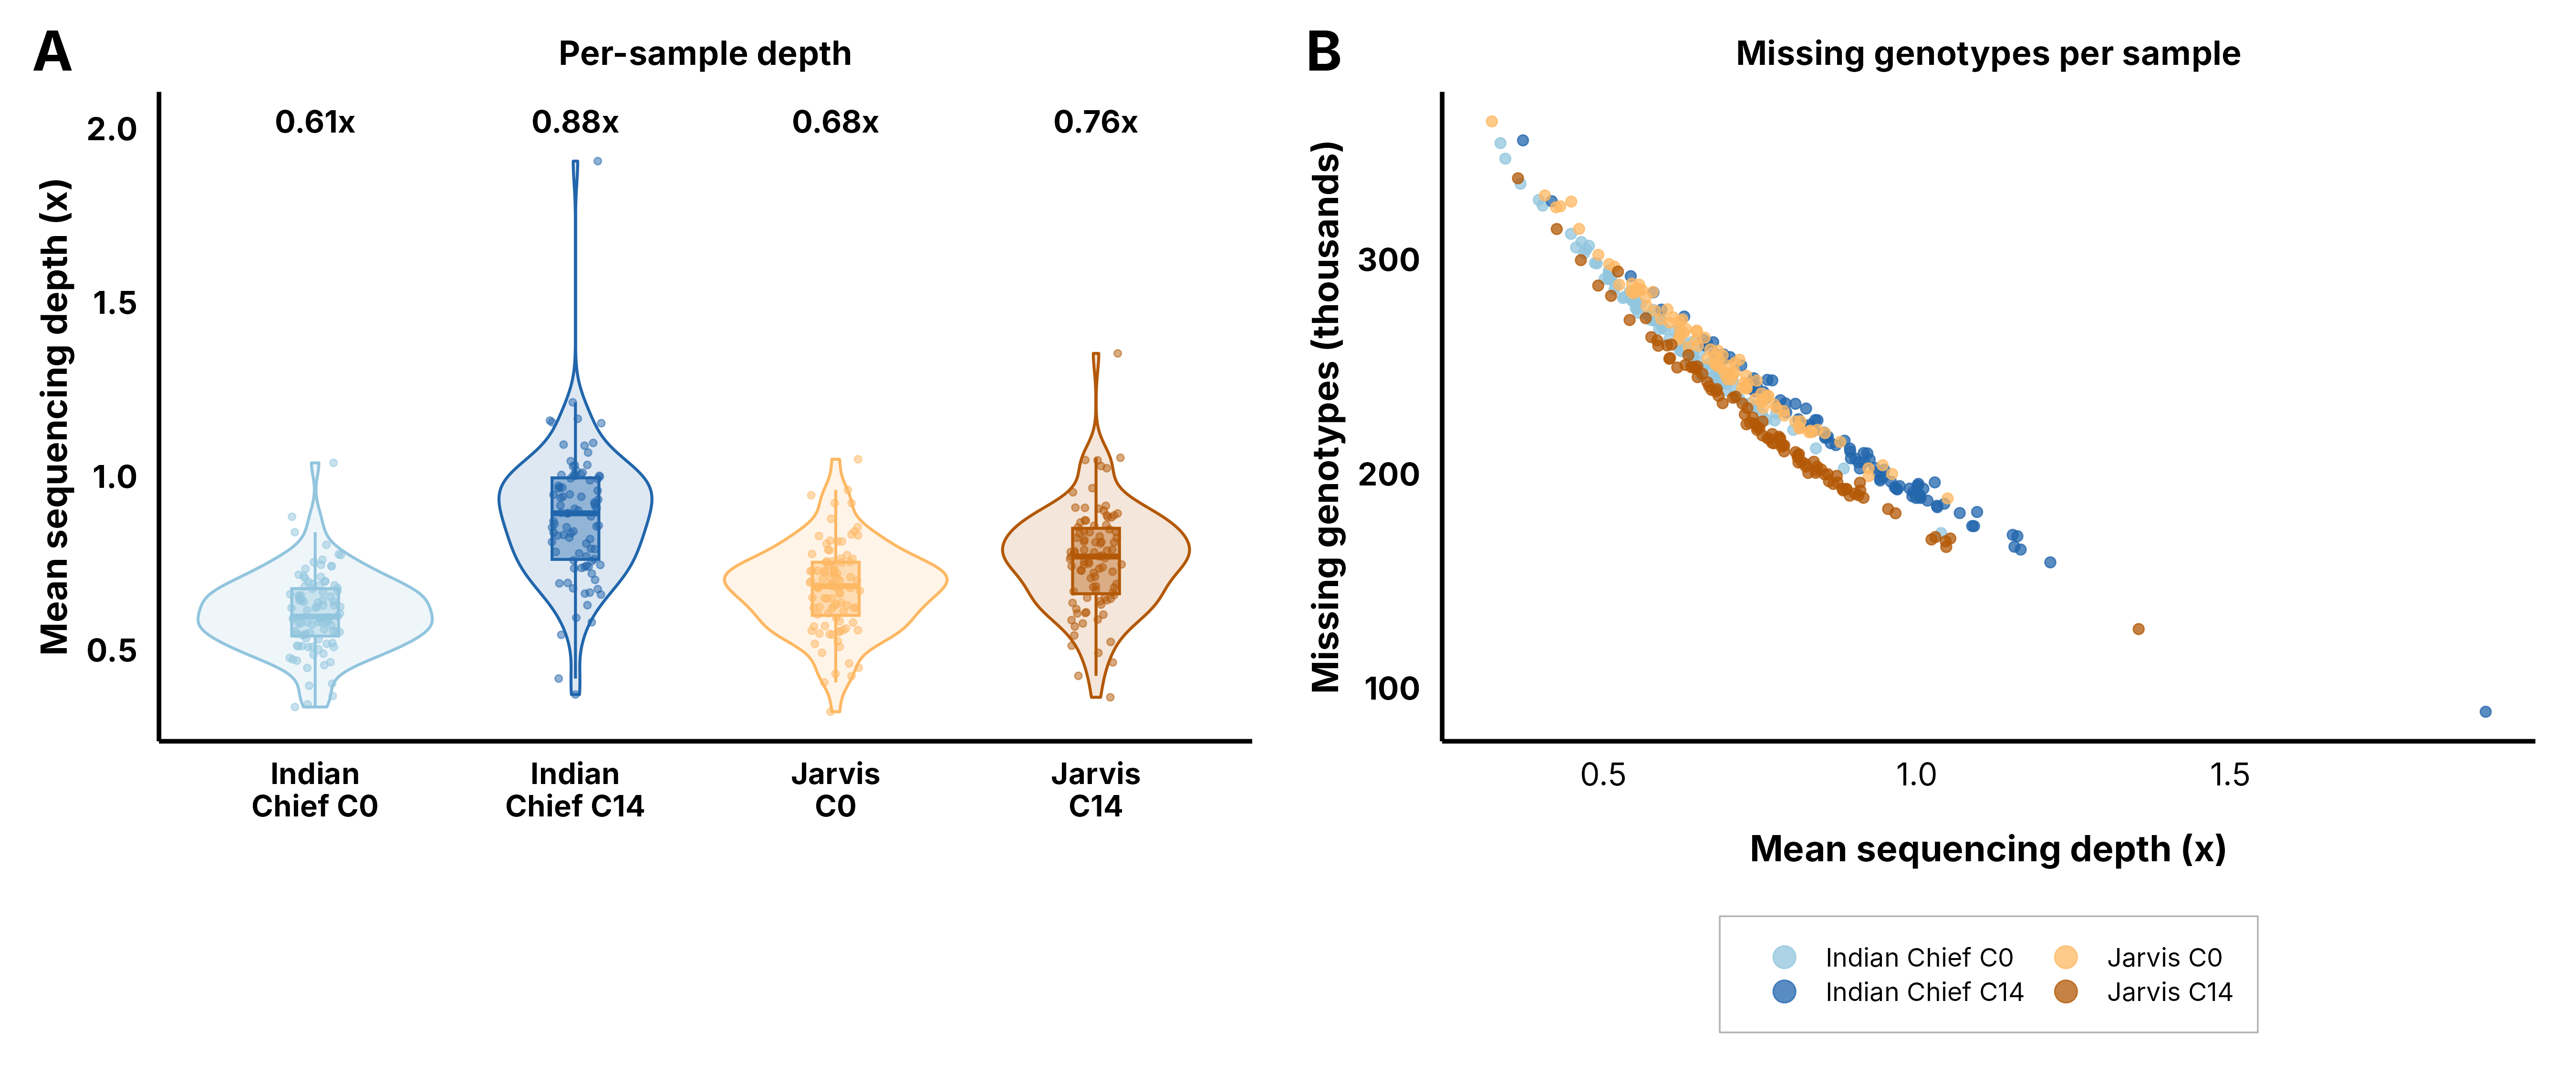
\includegraphics[width=\textwidth]{final/supp_figs/SuppFig_seq_statistics_sample_level.png}
    \caption{\textbf{Per-sample sequencing depth in the Indian Chief and Jarvis skim-sequencing data.} \textbf{(A)} Mean sequencing depth per individual for each population and cycle; numbers give group means. \textbf{(B)} Number of missing genotypes (of 512,667 filtered SNPs) per individual against its mean depth.}
    \label{fig:supp_seq_sample}
\end{figure*}


% =========================
% SUPP FIGURE S12
% =========================                                                  
\begin{figure*}[!htbp]
    \centering
    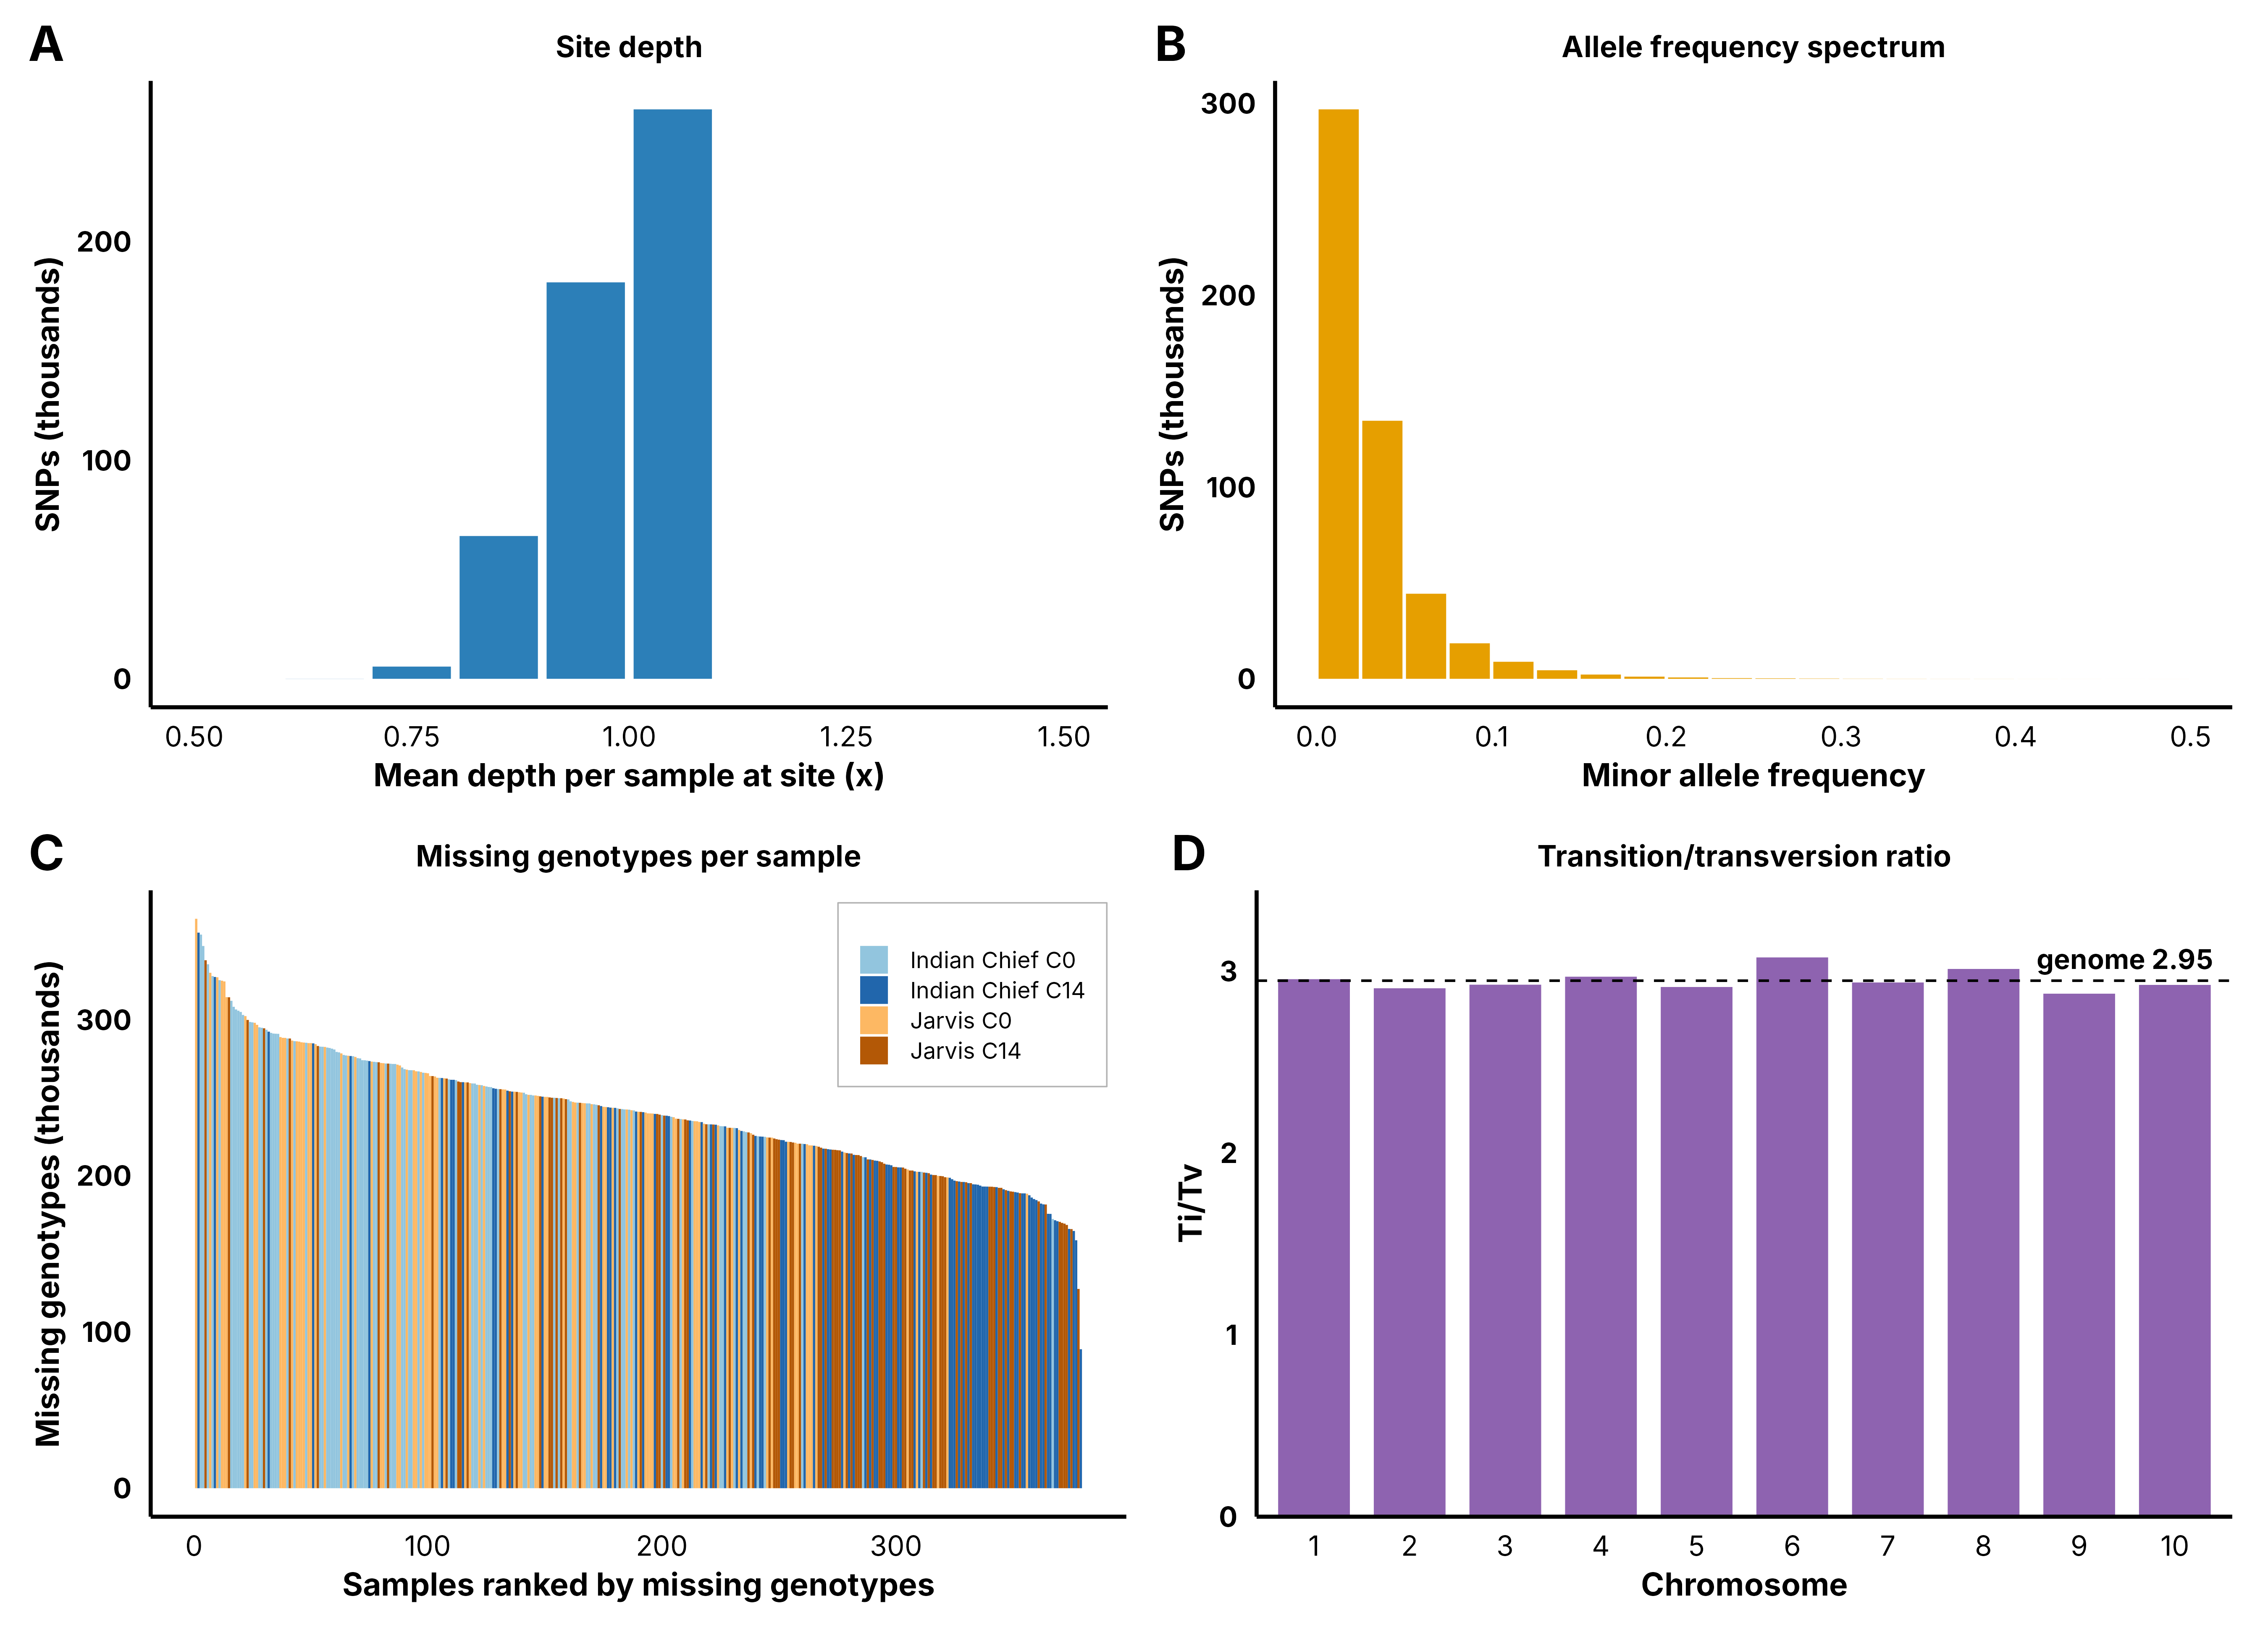
\includegraphics[width=\textwidth]{final/supp_figs/SuppFig_seq_statistics_variant_level.png}
    \caption{\textbf{Quality summaries for the 512,667 filtered SNPs.} \textbf{(A)} Mean depth per individual at each SNP (total site depth divided by 379). \textbf{(B)} Minor allele frequency spectrum, from called genotypes. \textbf{(C)} Missing genotypes per individual, ranked and colored by population and cycle. \textbf{(D)} Transition/transversion ratio by chromosome; dashed line, genome-wide value.}
    \label{fig:supp_seq_variant}
\end{figure*}

% =========================
% SUPP FIGURE S13
% =========================
\begin{figure*}[!htbp]
    \centering
    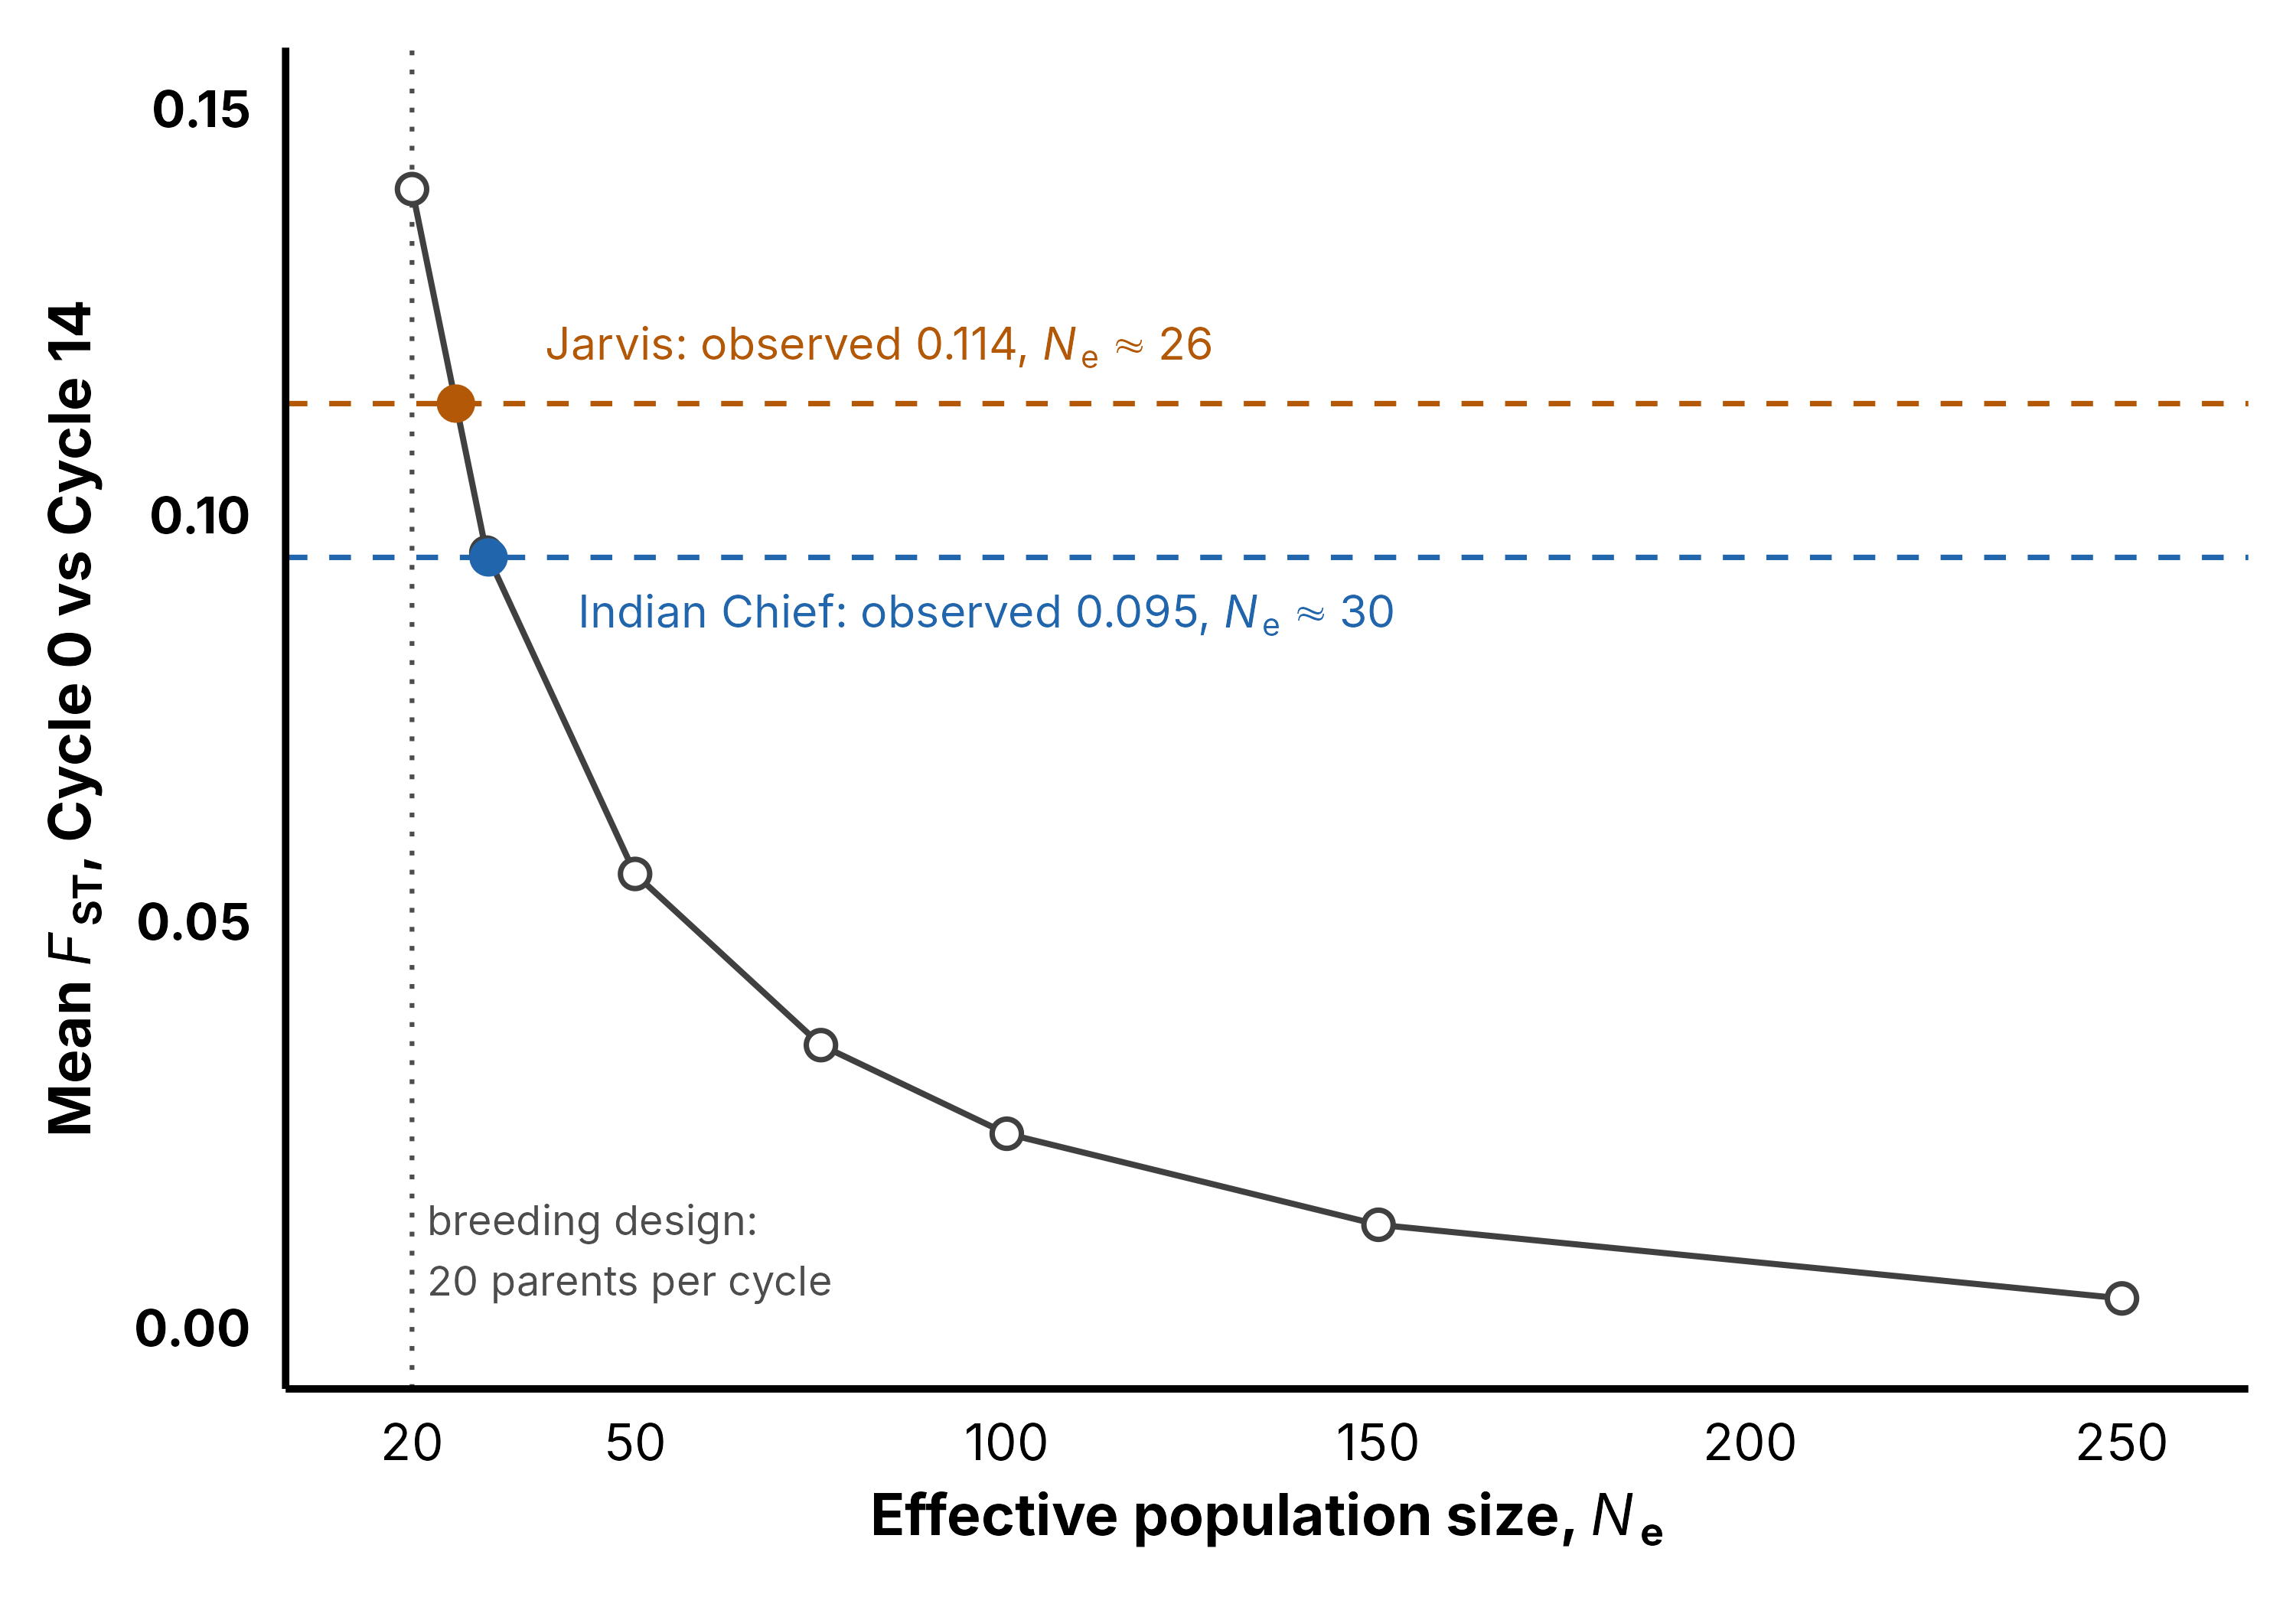
\includegraphics[width=0.75\textwidth]{final/supp_figs/SuppFig_IC_J_Ne_drift.png}
    \caption{\textbf{Effective population size of the Indian Chief and Jarvis recurrent-selection populations.} Genome-wide mean $F_{ST}$ between Cycle~0 and Cycle~14 expected under neutral Wright--Fisher drift for 14 generations across a range of effective population sizes ($N_e$; open circles), starting from the observed Cycle~0 allele frequencies and resampling the number of individuals sequenced at each site. Dashed lines give the observed values (Indian Chief 0.095, Jarvis 0.114), and filled circles mark the implied $N_e$, obtained by linear interpolation. The dotted line marks $N_e = 20$, the value expected when the 20 parents intermated in each cycle contribute equally.}
    \label{fig:supp_ne_drift}
\end{figure*}

% =========================
% SUPP FIGURE S14
% =========================
\begin{figure*}[!htbp]
    \centering
    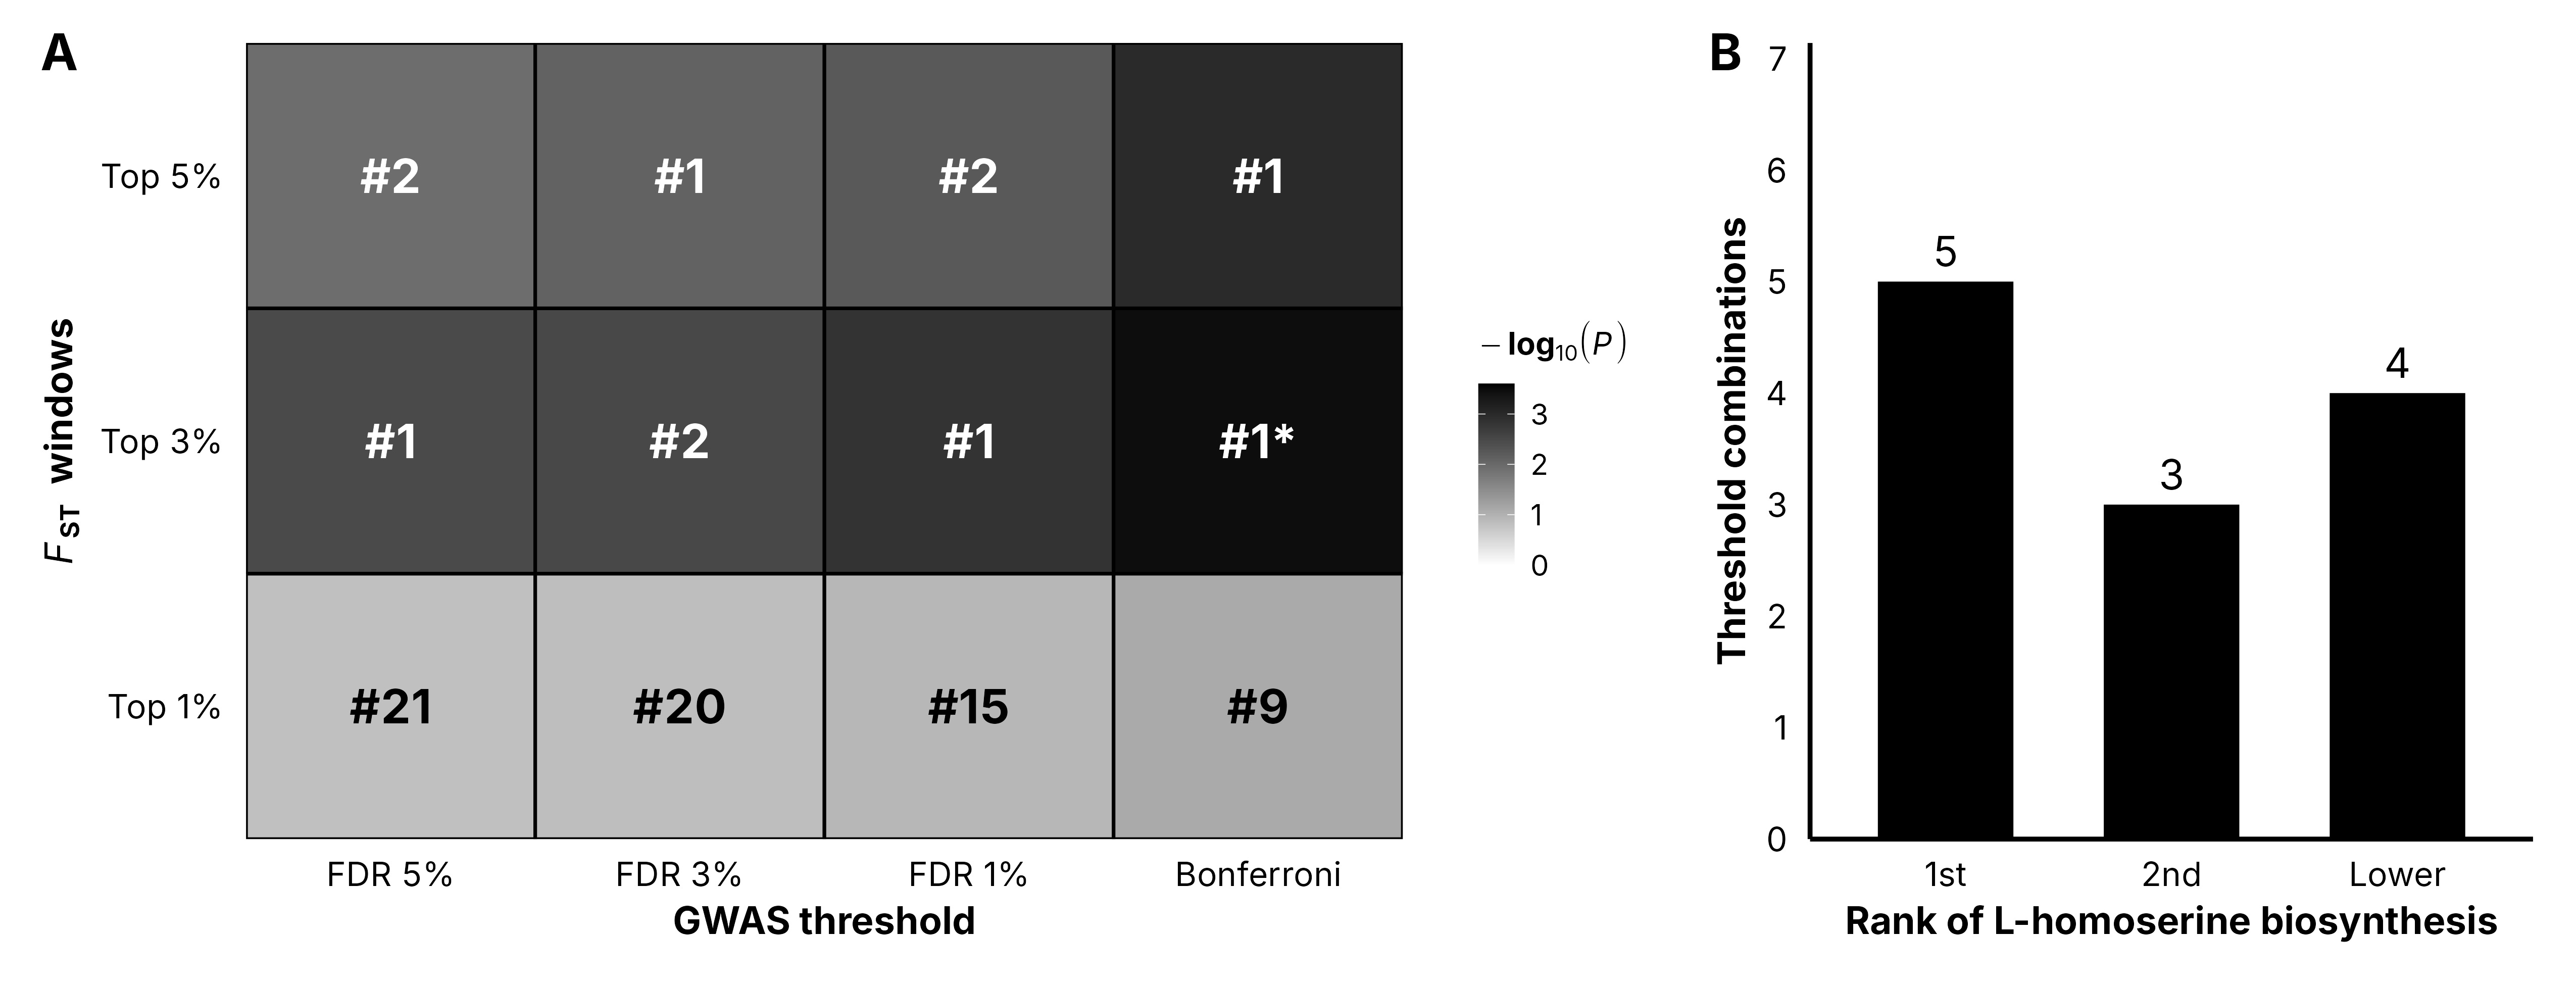
\includegraphics[width=0.75\textwidth]{final/supp_figs/SuppFig_pathway_threshold_sensitivity.png}
    \caption{\textbf{Sensitivity of the pathway recurrence test to candidate thresholds.} \textbf{(A)} L-homoserine biosynthesis across 12 combinations of GWAS threshold (columns, applied to both the amino acid and soil-N GWAS) and $F_{ST}$ window threshold (rows, Indian Chief and Jarvis). Shading gives $-\log_{10}$ of the pathway-specific permutation-based empirical $P$, labels give the rank of L-homoserine biosynthesis among the 468 CornCyc pathways, and an * marks $P < 0.05$ after correction across all pathways. At the top 1\%, the Indian Chief and Jarvis genes were no longer included and the pathway was hit by two analyses. \textbf{(B)} Number of the 12 combinations in which L-homoserine biosynthesis ranked first, second, or lower. Permutations, 20,000 per combination and 200,000 for the Bonferroni sets with the top 5\% and 3\% of windows.}
    \label{suppfig:pathway_thresholds}
\end{figure*}

\clearpage


\clearpage
\newpage

% --- Table S1 ---
\paragraph*{S1 Table.}
\phantomsection
\makeatletter
\def\@currentlabelname{S1 Table}
\makeatother
\label{S1_Table}
\textbf{Free amino acid phenotypes across the Goodman--Buckler Association Panel.} Genotype-level values of the 78 amino acid phenotypes used for GWAS for 280 of the 282 lines (two years $\times$ two blocks, Columbia, Missouri): 20 absolute FAA concentrations, six biosynthetic-family composites, 20 ratios to the total free pool, 25 ratios to the family composite, four ratios between amino acids (N.D, N.E, N.Q, Q.E) and three whole-pool traits. Trait codes are defined in Supplementary Table~S2.

% --- Table S2 ---
\paragraph*{S2 Table.}
\phantomsection
\makeatletter
\def\@currentlabelname{S2 Table}
\makeatother
\label{S2_Table}
\textbf{Amino acid trait definitions.} Code and description of each of the 78 amino acid phenotypes in Supplementary Table~S1.

% --- Table S3 ---
\paragraph*{S3 Table.}
\phantomsection
\makeatletter
\def\@currentlabelname{S3 Table}
\makeatother
\label{S3_Table}
\textbf{Abundance, variability, and heritability of the 20 free amino acids.} For each FAA across 280 lines (278 for Tyr): median, mean, standard deviation, minimum, maximum, fold range, coefficient of variation, line mean broad-sense heritability ($H^2$), genomic heritability ($h^2$), and the Spearman correlation between 2017 and 2018 line means for the lines grown in both years.

% --- Table S4 ---
\paragraph*{S4 Table.}
\phantomsection
\makeatletter
\def\@currentlabelname{S4 Table}
\makeatother
\label{S4_Table}
\textbf{Heritability of free and protein-bound amino acid traits.} Line-mean and Cullis broad-sense heritability ($H^2$) and genomic heritability ($h^2$, with 95\% interval and permuted-phenotype null) for 40 FAA and 76 PBAA traits, with sample sizes and the Spearman correlation between 2017 and 2018 line means.

% --- Table S5 ---
\paragraph*{S5 Table.}
\phantomsection
\makeatletter
\def\@currentlabelname{S5 Table}
\makeatother
\label{S5_Table}
\textbf{Free vs.\ protein-bound amino acid pools.} Paired comparison of FAA and PBAA pools across matched lines for the total amino acid pool, the amino acid-derived N proxy, the proline fraction and the Asx + Glx + basic fraction (matched denominators): mean, median, standard deviation and coefficient of variation of each pool, fold difference and paired Wilcoxon $P$.

% --- Table S6 ---
\paragraph*{S6 Table.}
\phantomsection
\makeatletter
\def\@currentlabelname{S6 Table}
\makeatother
\label{S6_Table}
\textbf{Amino acid GWAS candidate genes.} All phenotype $\times$ SNP $\times$ gene combinations for SNPs significant at 5\% Benjamini--Hochberg FDR (per phenotype and model; MLM, BLINK, FarmCPU) within 25~kb of a B73 RefGen\_v5 gene: 1,811 SNPs, 71 phenotypes, 3,693 genes. Includes significant models, lowest $P$ and FDR, whether the SNP is significant in $\geq$2 models, gene coordinates and distance. Positions are given on AGPv4 (\texttt{Pos\_v4}, the coordinate of the genotype data) and B73 RefGen\_v5 (\texttt{Pos\_v5}, lifted with the chain file; \texttt{lift} = \texttt{gap} marks SNPs placed at the nearest aligned base); marker names carry the older AGPv3 coordinate.

% --- Table S7 ---
\paragraph*{S7 Table.}
\phantomsection
\makeatletter
\def\@currentlabelname{S7 Table}
\makeatother
\label{S7_Table}
\textbf{Amino acid GWAS loci.} The 2,152 loci were formed by merging FDR-significant SNP within 25 kb across phenotypes, with B73 RefGen\_v5 coordinates, numbers of SNPs and phenotypes, best $P$, lead SNP (AGPv4 and v5 positions), supporting models, genes within 25 kb (or the nearest gene and its distance when none), top gene and its PANTHER family and GO terms.

% --- Table S8 ---
\paragraph*{S8 Table.}
\phantomsection
\makeatletter
\def\@currentlabelname{S8 Table}
\makeatother
\label{S8_Table}
\textbf{Genes in the chromosome~3 Asp/Pro QTL interval of the B64 $\times$ CML14 population.} The 1,578 B73 RefGen\_v5 genes (1,386 protein-coding and 192 non-coding) within the 1.5-LOD support intervals (chr3:14.37--143.31~Mb) of the shared free Asp and Pro QTL (peak at 35.99~Mb), with gene coordinates, biotype, membership in the Asp and Pro intervals, distance to the QTL peak, gene name, PANTHER family, protein class, GO terms, kernel expression from qTeller \citep{qteller}, and overlap with candidates from the amino acid GWAS, soil N GWAS, and Indian Chief and Jarvis $F_{ST}$ scans.

% --- Table S9 ---
\paragraph*{S9 Table.}
\phantomsection
\makeatletter
\def\@currentlabelname{S9 Table}
\makeatother
\label{S9_Table}
\textbf{Soil N GWAS candidate genes.} The 448 B73 RefGen\_v5 genes within 25~kb of the 216 soil-N SNPs (0--5~cm, 5\% FDR) that lie near a gene, one row per gene $\times$ SNP, with SNP statistics, overlap with other environmental GWAS, gene coordinates, distance, name, PANTHER family, protein class and GO terms.

% --- Table S10 ---
\paragraph*{S10 Table.}
\phantomsection
\makeatletter
\def\@currentlabelname{S10 Table}
\makeatother
\label{S10_Table}
\textbf{Environmental GWAS overlap test.} Observed vs.\ expected numbers of shared FDR-significant SNPs (MLM, BLINK and FarmCPU combined) for each site variable against the union of geographic variables (latitude, longitude, elevation; the variable itself excluded), and for soil N (0--5~cm) against each other variable. Expected $= n_1 n_2 / M$ with $M = 495{,}755$; one-sided hypergeometric $P$.

% --- Table S11 ---
\paragraph*{S11 Table.}
\phantomsection
\makeatletter
\def\@currentlabelname{S11 Table}
\makeatother
\label{S11_Table}
\textbf{Soil-N GWAS SNPs and their overlap with other environmental GWAS.} All 234 SNPs significant for soil N (0--5~cm) at 5\% FDR in MLM, BLINK or FarmCPU, with $P$ per model, MAF, number of models, whether each SNP is also FDR-significant in the GWAS of CEC, aridity, elevation, latitude, longitude, soil pH and soil N at 5--15~cm, and genes within 25~kb with the nearest gene's annotation.

% --- Table S12 ---
\paragraph*{S12 Table.}
\phantomsection
\makeatletter
\def\@currentlabelname{S12 Table}
\makeatother
\label{S12_Table}
\textbf{Genotype--environment correlation test for soil-N SNPs.} For each of the 234 soil-N SNPs, the Pearson correlation between genotype and soil N (0--5 and 5--15~cm), latitude, longitude, elevation, soil pH, CEC and aridity across 3,107 accessions; the SNP's genome-wide rank for each variable (\% of 495,755 SNPs with a stronger correlation); the most strongly correlated non-N variable; and the call: linked to environment (top 1\% for any non-N variable), not linked, or inconclusive (weak soil-N correlation, outside the top 5\%).

% --- Table S13 ---
\paragraph*{S13 Table.}
\phantomsection
\makeatletter
\def\@currentlabelname{S13 Table}
\makeatother
\label{S13_Table}
\textbf{Expectation test for the genotype–environment correlation.} Share of SNPs in the top 1\% of the genome for at least one geographic variable (latitude, longitude, elevation) or at least one of six non-N variables (adding soil pH, CEC, and aridity), for the whole genome, for SNPs in the top 1\% for correlation with soil N, for all soil N GWAS SNPs, and for those significant in $\geq$2 models, with binomial tests against the whole genome and against the soil N-correlated SNPs.

% --- Table S14 ---
\paragraph*{S14 Table.}
\phantomsection
\makeatletter
\def\@currentlabelname{S14 Table}
\makeatother
\label{S14_Table}
\textbf{Free amino acid metrics in Indian Chief and Jarvis, Cycle~0 vs. Cycle~14.} Eight pre-specified FAA metrics (total FAA per mg sample; Pro, Asn, Asp, Gln, and Gly fractions of total FAA; Asn + Gln + Arg + Lys + His per mg; FAA-derived N per mg) per population: biological-sample sizes, means, and medians per cycle, two-sided Wilcoxon rank-sum $P$, Benjamini--Hochberg-adjusted $P$ across the eight metrics, Cliff's $\delta$ (C14 vs. C0) and direction of change.

% --- Table S15 ---
\paragraph*{S15 Table.}
\phantomsection
\makeatletter
\def\@currentlabelname{S15 Table}
\makeatother
\label{S15_Table}
\textbf{Amino acid composition in Indian Chief and Jarvis, Cycle~0 vs.\ Cycle~14.} For each of the 20 free and 16 protein-bound amino acids, its fraction of the total pool per population and cycle: sample sizes, means, medians, Wilcoxon rank-sum $P$, Benjamini--Hochberg-adjusted $P$ across the amino acids of that pool, Cliff's $\delta$ and direction of change.

% --- Table S16 ---
\paragraph*{S16 Table.}
\phantomsection
\makeatletter
\def\@currentlabelname{S16 Table}
\makeatother
\label{S16_Table}
\textbf{Protein-bound amino acid metrics in Indian Chief and Jarvis, Cycle~0 vs.\ Cycle~14.} Six PBAA metrics (total PBAA per mg sample; proline, Asx and Glx fractions; Asx + Glx + Arg + Lys + His per mg; estimated PBAA-derived N per mg, with Asx and Glx at 1.5 N), with the same statistics as Supplementary Table~S14 and Benjamini--Hochberg adjustment across the six.

% --- Table S17 ---
\paragraph*{S17 Table.}
\phantomsection
\makeatletter
\def\@currentlabelname{S17 Table}
\makeatother
\label{S17_Table}
\textbf{Amino acid-derived N per mg sample in Indian Chief and Jarvis.} FAA-derived N, estimated PBAA-derived N, and estimated total amino acid-derived N per mg sample, per population and cycle, with Wilcoxon rank-sum $P$ and Benjamini--Hochberg-adjusted $P$ across the three measures. 

% --- Table S18 ---
\paragraph*{S18 Table.}
\phantomsection
\makeatletter
\def\@currentlabelname{S18 Table}
\makeatother
\label{S18_Table}
\textbf{Indian Chief $F_{ST}$ windows, Cycle~0 vs. Cycle~14.} All 2,162 GenWin spline windows with chromosome, window number, start and end (B73 RefGen\_v5), number of sites, mean per-site $F_{ST}$, whether the window is in the top 5\% ($F_{ST} \geq 0.157$), and the number and IDs of overlapping genes.

% --- Table S19 ---
\paragraph*{S19 Table.}
\phantomsection
\makeatletter
\def\@currentlabelname{S19 Table}
\makeatother
\label{S19_Table}
\textbf{Jarvis $F_{ST}$ windows, Cycle~0 vs.\ Cycle~14.} All 2,151 GenWin spline windows, with the same columns as Supplementary Table~S18 (top 5\%: $F_{ST} \geq 0.178$).

% --- Table S20 ---
\paragraph*{S20 Table.}
\phantomsection
\makeatletter
\def\@currentlabelname{S20 Table}
\makeatother
\label{S20_Table}
\textbf{Indian Chief candidate genes in top-5\% $F_{ST}$ windows.} The 2,001 genes overlapping the 109 top-5\% windows, with gene name, window coordinates and $F_{ST}$, whether the gene also lies in a top-5\% Jarvis window (\texttt{shared\_with\_other\_population}), PANTHER family and protein class, and Gene Ontology molecular function, biological process, and cellular component terms. Genes in the same window share one $F_{ST}$ value and are not independent.

% --- Table S21 ---
\paragraph*{S21 Table.}
\phantomsection
\makeatletter
\def\@currentlabelname{S21 Table}
\makeatother
\label{S21_Table}
\textbf{Jarvis candidate genes in top-5\% $F_{ST}$ windows.} The 1,179 genes overlap 106 of the 108 top-5\% windows (the other two contain no genes), with the same columns as Supplementary Table~S20.

% --- Table S22 ---
\paragraph*{S22 Table.}
\phantomsection
\makeatletter
\def\@currentlabelname{S22 Table}
\makeatother
\label{S22_Table}
\textbf{Expression responses of candidate genes to N supply in public maize RNA-seq.} Reanalysis of published maize RNA-seq studies of root, leaf, shoot, and whole-seedling tissue (no kernel data) for the candidate genes named in the text and \textit{ASN3}.

\end{document}
